\documentclass[journal,letterpaper,onecolumn,twoside,nofonttune]{IEEEtran}
%\documentclass[conference,letterpaper]{IEEEtran}

\usepackage[utf8]{inputenc}
\usepackage[T1]{fontenc}
\usepackage{url}
\usepackage{ifthen}
\usepackage{cite}
\usepackage[cmex10]{amsmath}
\interdisplaylinepenalty=2500
\usepackage{balance}

\usepackage{amsmath}
\usepackage{amsthm}
\usepackage{amsfonts}
\usepackage{amssymb}
\usepackage{mathtools}
\usepackage{color}
\usepackage{verbatim}
\usepackage[normalem]{ulem}
\usepackage{enumitem}
\usepackage{hyperref}
\usepackage[ruled,vlined]{algorithm2e}
\usepackage{algpseudocode}
\usepackage{mathrsfs}

\usepackage{caption}
\captionsetup{justification=centering}

% - - - - - - - - - - - - - - -

\definecolor{purple}{rgb}{0.5, 0.0, 0.5}
\definecolor{dark_green}{rgb}{0.0, 0.5, 0.0}
\definecolor{dyellow}{rgb}{0.99, 0.93, 0.0}
\definecolor{amaranth}{rgb}{0.9, 0.17, 0.31}

\newcommand{\red}{\color{red}}
\newcommand{\green}{\color{green}}
\newcommand{\dgreen}{\color{dark_green}}
\newcommand{\blue}{\color{blue}}
\newcommand{\cyan}{\color{cyan}}
\newcommand{\purple}{\color{purple}}
\newcommand{\white}{\color{white}}
\newcommand{\yellow}{\color{yellow}}
\newcommand{\magenta}{\color{magenta}}
\newcommand{\dyellow}{\color{aureolin}}
\newcommand{\diffred}{\color{amaranth}}  % different

\newcommand{\N}{\mathbb{N}}
\newcommand{\Z}{\mathbb{Z}}
\newcommand{\Q}{\mathbb{Q}}
\newcommand{\R}{\mathbb{R}}
\newcommand{\C}{\mathbb{C}}
\newcommand{\Ham}{\mathbb{H}}
\newcommand{\Pspace}{\mathbb{P}}
\newcommand{\RP}{\mathbb{RP}}
\newcommand{\sphere}{\mathbb{S}}
\newcommand{\F}{\mathbb{F}}
\newcommand{\E}{\mathbb{E}}
\newcommand{\pr}{\mathfrak{p}}
\newcommand{\m}{\mathfrak{m}}
\newcommand{\al}{\mathfrak{a}}
\newcommand{\eq}{\equiv}
\newcommand{\htwo}{\-\hspace{2cm}}
\newcommand{\rpm}{\raisebox{.2ex}{$\scriptstyle\pm$}}
\newcommand\norm[1]{\left\lVert#1\right\rVert}

\newcommand{\ow}{\mathcal{O}}
\newcommand{\A}{\mathcal{A}}
\newcommand{\B}{\mathcal{B}}
\newcommand{\Cc}{\mathcal{C}}
\newcommand{\D}{\mathcal{D}}
\newcommand{\Ee}{\mathcal{E}}
\newcommand{\Ff}{\mathcal{F}}
\newcommand{\G}{\mathcal{G}}
\newcommand{\I}{\mathcal{I}}
\newcommand{\J}{\mathcal{J}}
\newcommand{\K}{\mathcal{K}}
\newcommand{\Kbar}{\bar{\mathcal{K}}}
\newcommand{\M}{\mathcal{M}}
\newcommand{\Nn}{\mathcal{N}}
\newcommand{\Qq}{\mathcal{Q}}
\newcommand{\lan}{\mathcal{L}}
\newcommand{\lag}{\mathscr{L}}
\newcommand{\Scal}{\mathcal{S}}
\newcommand{\Tcal}{\mathcal{T}}
\newcommand{\Uu}{\mathcal{U}}
\newcommand{\Ww}{\mathcal{W}}
\newcommand{\Eeb}{\bar{\mathcal{E}}}
\newcommand{\Ffb}{\bar{\mathcal{F}}}
\newcommand{\Sbar}{\bar{\mathcal{S}}}
\newcommand{\Tbar}{\bar{\mathcal{T}}}
\newcommand{\ab}{\bold{a}}
\newcommand{\bb}{\bold{b}}
\newcommand{\cb}{\bold{c}}
\newcommand{\db}{\bold{d}}
\newcommand{\dhat}{\hat{d}}
\newcommand{\dt}{\tilde{d}}
\newcommand{\dbt}{\tilde{\db}}
\newcommand{\dbar}{\bar{d}}
\newcommand{\eb}{\bold{e}}
\newcommand{\fb}{\bold{f}}
\newcommand{\fbh}{\hat{\bold{f}}}
\newcommand{\gb}{\bold{g}}
\newcommand{\gbh}{\hat{\bold{g}}}
\newcommand{\hb}{\bold{h}}
\newcommand{\hbh}{\hat{\bold{h}}}
\newcommand{\mb}{\bold{m}}
\newcommand{\Qbar}{\bar{Q}}
\newcommand{\Qh}{\hat{Q}}
\newcommand{\qbar}{\bar{q}}
\newcommand{\Ub}{\bold{U}}
\newcommand{\Ubt}{\tilde{\Ub}}
\newcommand{\ub}{\bold{u}}
\newcommand{\Vb}{\bold{V}}
\newcommand{\Vbh}{\hat{\bold{V}}}
\newcommand{\vb}{\bold{v}}
\newcommand{\xb}{\bold{x}}
\newcommand{\xbt}{\tilde{\xb}}
\newcommand{\xbh}{\hat{\xb}}
\newcommand{\Xt}{\tilde{X}}
\newcommand{\yb}{\bold{y}}
\newcommand{\yt}{\tilde{y}}
\newcommand{\ybt}{\tilde{\yb}}
\newcommand{\ybh}{\hat{\yb}}
\newcommand{\Ab}{\bold{A}}
\newcommand{\Bb}{\bold{B}}
\newcommand{\Bbbar}{\bar{\bold{B}}}
\newcommand{\Cb}{\bold{C}}
\newcommand{\Db}{\bold{D}}
\newcommand{\Dbwt}{\widetilde{\Db}}
\newcommand{\Eb}{\bold{E}}
\newcommand{\Ebt}{\tilde{\bold{E}}}
\newcommand{\Ebwt}{\widetilde{\bold{E}}}
\newcommand{\Ebb}{\Eb_\mathrm{b}}
\newcommand{\Fb}{\bold{F}}
\newcommand{\Gb}{\bold{G}}
\newcommand{\Gbp}{\bold{G}_\mathrm{p}}
\newcommand{\Hb}{\bold{H}}
\newcommand{\Ib}{\bold{I}}
\newcommand{\Hbh}{\hat{\bold{H}}}
\newcommand{\Hbt}{\tilde{\bold{H}}}
\newcommand{\Mb}{\bold{M}}
\newcommand{\Tb}{\bold{T}}
\newcommand{\tb}{\bold{t}}
\newcommand{\Pb}{\bold{P}}
\newcommand{\Qb}{\bold{Q}}
\newcommand{\Qt}{\tilde{Q}}
\newcommand{\Rb}{\bold{R}}
\newcommand{\RHb}{\bold{R}_{\bold{H}}}
\newcommand{\Sb}{\bold{S}}
\newcommand{\Sigb}{\bold{\Sigma}}
\newcommand{\Sbt}{\tilde{\Sb}}
\newcommand{\Sbwt}{\widetilde{\Sb}}
\newcommand{\Sbh}{\hat{\Sb}}
\newcommand{\Abh}{\hat{\Ab}}
\newcommand{\Abw}{\Ab_{\wb}}
\newcommand{\Abph}{\hat{\Ab}_\mathrm{p}}
\newcommand{\Abwh}{\hat{\Ab}_{\wb}}
\newcommand{\Xbph}{\hat{\Xb}_\mathrm{p}}
\newcommand{\Sbb}{\Sb_\mathrm{b}}
\newcommand{\Sbp}{\Sb_\mathrm{p}}
\newcommand{\Sbw}{\Sbwt_{\wb}}
\newcommand{\sbold}{\bold{s}}
\newcommand{\wb}{\bold{w}}
\newcommand{\Wb}{\bold{W}}
\newcommand{\Wbb}{\bar{\bold{W}}}
\newcommand{\zb}{\bold{z}}
\newcommand{\Zb}{\bold{Z}}
\newcommand{\Xb}{\bold{X}}
\newcommand{\Yb}{\bold{Y}}
\newcommand{\At}{\tilde{A}}
\newcommand{\Abt}{\tilde{\Ab}}
\newcommand{\at}{\tilde{a}}
\newcommand{\abt}{\tilde{\ab}}
\newcommand{\Bt}{\tilde{B}}
\newcommand{\Bbt}{\tilde{\Bb}}
\newcommand{\Bbh}{\hat{\Bb}}
\newcommand{\bt}{\tilde{b}}
\newcommand{\bbt}{\tilde{\bb}}
\newcommand{\bbh}{\hat{\bb}}
\newcommand{\Ct}{\tilde{C}}
\newcommand{\Cbt}{\bold{\tilde{C}}}
\newcommand{\Dt}{\tilde{\mathcal{D}}}
\newcommand{\Rh}{\hat{R}}
\newcommand{\Rt}{\tilde{R}}
\newcommand{\rh}{\hat{r}}
\newcommand{\rt}{\tilde{r}}
\newcommand{\Rbt}{\bold{\tilde{R}}}
\newcommand{\gt}{\tilde{g}}
\newcommand{\gh}{\hat{g}}
\newcommand{\Hh}{\hat{H}}
\newcommand{\Xbt}{\tilde{\Xb}}
\newcommand{\Xbh}{\hat{\Xb}}
\newcommand{\gammab}{\bar{gamma}}
\newcommand{\Thb}{\bold{\Theta}}
\newcommand{\Omb}{\bold{\Omega}}
\newcommand{\Ombb}{\bar{\bold{\Omega}}}
\newcommand{\Ombwt}{\widetilde{\Omb}}
\newcommand{\Ombw}{\Omb_{\wb}}
\newcommand{\Pib}{\bar{\Pi}}
\newcommand{\Pih}{\hat{\Pi}}
\newcommand{\Pis}{\Pi^{\star}}
\newcommand{\Pit}{\tilde{\Pi}}
\newcommand{\PsiB}{\bold{\Psi}}
\newcommand{\PsiBb}{\bar{\PsiB}}
\newcommand{\phit}{\tilde{\phi}}
\newcommand{\psiv}{\vec{\psi}}
\newcommand{\wbt}{\tilde{\wb}}
\newcommand{\Wbt}{\tilde{\Wb}}
\newcommand{\psit}{\tilde{\psi}}
\newcommand{\Ft}{\tilde{F}}
\newcommand{\ellt}{\tilde{\ell}}
\newcommand{\Var}{\mathrm{Var}}
\newcommand{\rank}{\mathrm{rank}}
\newcommand{\lcm}{\mathrm{lcm}}
\newcommand{\diag}{\mathrm{diag}}
\newcommand{\err}{\mathrm{err}}
\newcommand{\image}{\mathrm{im}}
\newcommand{\SVD}{\mathrm{SVD}}
\newcommand{\QR}{\mathrm{QR}}
\newcommand{\LU}{\mathrm{LU}}

\newcommand{\qvec}[1]{\textbf{\textit{#1}}}

\DeclarePairedDelimiter\ceil{\lceil}{\rceil}
\DeclarePairedDelimiter\floor{\lfloor}{\rfloor}
\DeclarePairedDelimiter{\nint}\lfloor\rceil

\DeclarePairedDelimiter\bceil{\big\lceil}{\big\rceil}
\DeclarePairedDelimiter\bfloor{\big\lfloor}{\big\rfloor}

\newtheorem{Thm}{Theorem}
\newtheorem{Cor}{Corollary}
\newtheorem{Prop}{Proposition}
\newtheorem{Lemma}{Lemma}
\newtheorem{Def}{Definition}
\newtheorem{Rmk}{Remark}

\newcommand{\ind}{\text{\color{white}.$\quad$}}
\DeclareMathOperator*{\argmin}{arg\,min}

% ------------------------------------------------------------
\begin{document}
\title{Gradient Coding through Iterative Block Leverage Score Sampling}
%\title{Gradient Coding through Block Leverage Score Sampling and Iterative Sketching}

\author{$\textbf{Neophytos Charalambides}^{\mu}$, $\textbf{Mert Pilanci}^{\sigma}$, \textbf{and} $\textbf{Alfred O. Hero III}^{\mu}$\\
$\text{\white.}^{\mu}$EECS Department University of Michigan $\text{\white.}^{\sigma}$EE Department Stanford University\\
  Email: \texttt{neochara@umich.edu}, \texttt{pilanci@stanford.edu}, \texttt{hero@umich.edu}
\thanks{This work was partially supported by grants ARO W911NF-15-1-0479 and DE NA0003921.}% <-this % stops a space
\vspace{-4mm}
}

\maketitle

\begin{abstract}
We generalize the leverage score sampling sketch for $\ell_2$-subspace embeddings, to accommodate sampling subsets of the transformed data, so that the sketching approach is appropriate for distributed settings. This is then used to derive an approximate coded computing approach for first-order methods; known as gradient coding, to accelerate linear regression in the presence of failures in distributed computational networks, \textit{i.e.} stragglers. We replicate the data across the distributed network, to attain the approximation guarantees through the induced sampling distribution. The significance and main contribution of this work, is that it unifies randomized numerical linear algebra with approximate coded computing, while attaining an induced $\ell_2$-subspace embedding through uniform sampling. The transition to uniform sampling is done without applying a random projection, as in the case of the subsampled randomized Hadamard transform. Furthermore, by incorporating this technique to coded computing, our scheme is an iterative sketching approach to approximately solving linear regression. We also propose weighting when sketching takes place through sampling with replacement, for further compression.% We also propose weighting for this non-uniform sampling technique for further compression, beyond that introduced by the sampling. What we propose also applies to other randomized sampling linear algebra algorithms, \textit{e.g.} matrix multiplication.
\end{abstract}
\vspace{3mm}

\begin{IEEEkeywords}
Leverage Score Sampling, Low-rank Approximations, Least-squares Regression, Sampling, Randomized Algorithms, Coded Computing, Stragglers, Erasure-Coding, Replication-Coding.
\end{IEEEkeywords}

% - - - - - - - - - - - - - - -
\section{Introduction}

In this work we bridge two disjoint areas, to accelerate first-order methods distributively, while focusing on linear regression. Specifically, we propose a framework in which \textit{Randomized Numerical Linear Algebra} (RandNLA) sampling algorithms can be used to devise \textit{Coded Computing} (CC) schemes. We focus on the task of $\ell_2$-\textit{subspace embedding} ($\ell_2$-s.e.); through leverage score sampling, and distributed gradient computation; which is referred to as \textit{gradient coding} (GC).

Traditional numerical linear algebra algorithms are deterministic. For example, inverting a full-rank matrix $\Ab\in\R^{N\times N}$ requires $O(N^3)$ arithmetic operations by performing Gaussian elimination, as does naive matrix multiplication. The fastest known algorithm which multiplies two $N\times N$ matrices, requires $O(N^{\omega})$ operations; for $\omega<2.373$ \cite{AV21,PV20}. Other important problems are computing the determinant, singular and eigenvalue decompositions, $\SVD$, $\QR$ and Cholesky factorizations.%while computing the Moore-Penrose pseudoinverse $\Ab^{\dagger}$ of a matrix $\Ab\in\R^{N\times d}$ requires itself $O(Nd^2+d^2)$ operations

Although these deterministic algorithms run in polynomial time and are numerically stable, their exponents make them prohibitive for many applications in scientific computing and machine learning, when $N$ is in the order of millions or billions \cite{MLG08,Mah12}. To circumvent this issue, one can perform these algorithms on a significantly smaller approximation. Specifically, for a matrix $\Sb\in\R^{r\times N}$ with $r\ll N$, we apply the deterministic algorithm on the surrogate $\Abh=\Sb\Ab\in\R^{r\times d}$. The matrix $\Sb$ is referred to as a ``dimension-reduction'' or a ``sketching'' matrix, and $\Abh$ is a ``sketch'' of $\Ab$, which contains as much information about $\Ab$ as possible. For instance, when multiplying $\Ab\in\R^{L\times N}$ and $\Bb\in\R^{N\times M}$, we apply a carefully chosen $\Sb\in\R^{r\times N}$ on each to get
$$ \overbrace{\begin{pmatrix} & & & & & & \\ & & & \Ab & & & \\ & & & & & & \end{pmatrix}}^{L\times N} \cdot \overbrace{\begin{pmatrix} & & \\ & & \\ & & \\ & \Bb & \\ & & \\ & & \\ & & \end{pmatrix}}^{N\times M} \approx \overbrace{\begin{pmatrix} & & & & \\ & & \Abh & & \\ & & & & \end{pmatrix}}^{L\times r} \cdot \overbrace{\begin{pmatrix} & & \\ & & \\ & \Bbh\ & \\ & & \\ & & \end{pmatrix}}^{r\times M} $$
for $\Abh=\Ab\Sb^\top$ and $\Bbh=\Sb\Bb$. Thus, naive matrix multiplication now requires $O(LMr)$ operations; instead of $O(LMN)$. Such approaches have been motivated by the Johnson-Lindenstrauss lemma \cite{JL84}, and require low complexity.%Such approaches have been motivated by the Johnson-Lindenstrauss lemma \cite{JL84}, and require low complexity to be constructed and applied.% It is also clear that the approximation $\Ab\Bb\approx\Ab\Bb$ implies $\Sb^\top\Sb\approx\Ib_N$. A popular way of constructing such an $\Sb$, is by the $CR$ matrix multiplication algorithm \cite{DK01,DKM06a,DKM06b}, in which an appropriate distribution based on the product of the Euclidean norms of the pairs of corresponding column vectors of $\Ab$ and row vectors of $\Bb$ is constructed. Then, $r$ many pair of rows are sampled with replacement according to this distribution and rescaled. The approximation is the sum of the rescaled rank-1 outer-products.

A multitude of other problems, such as $k$-means clustering \cite{BZMD14,CEMMP15,Cha20} and computing the $\SVD$ of a matrix \cite{DFKVV99,DFKVV04,DKM06a,DKM06b}, make use of this idea; in order to accelerate computing accurate approximate solutions. We refer the reader to the following monographs and comprehensive surveys on the rich development of RandNLA \cite{HMJ11,Mah12,Mah16,MM20,Wan15,Woo14,DM16}, an interdisciplinary field that exploits randomization as a computational resource; to develop improved algorithms for large-scale linear algebra problems.

The problem of $\ell_2$-s.e.; a form of spectral approximation of a matrix, has been extensively studied in RandNLA. The main techniques for constructing appropriate sketching $\ell_2$-s.e. matrices, are performing a random projection or row-sampling. Well-known choices of $\Sb$ for reducing the effective dimension $N$ to $r$ include: i) \textit{Gaussian projection}; for a matrix $\Thb\sim\Nn(0,1)$ define $\Sb=\frac{1}{\sqrt{r}}\Thb$, ii) \textit{leverage score sampling}; sample with replacement $r$ rows from the matrix according to its normalized leverage score distribution and rescale them appropriately, iii) \textit{Subsampled Hadamard Transform} (SRHT); apply a Hadamard transform and a random signature matrix to judiciously make the leverage scores approximately uniform and then follow similar steps to the leverage score sampling procedure.

In this paper, we first generalize ii) to appropriately sample \textit{submatrices} instead of rows to attain a $\ell_2$-s.e guarantee. We refer to such approaches as \textit{block sampling}. Throughout this paper, sampling is done with replacement (w.r.). Sampling blocks has been explored in ``block-iterative methods'' for solving systems of linear equations \cite{Elf80,Gut06,NT14,RN20}. Our motivation in dealing with blocks rather than individual vectors, is the availability to invoke results that can be used to characterize the approximations of distributed computing networks, to speed up first-order methods, as sampling individual rows/columns is prohibitive in real-world environments. This in turn leads to an \textit{iterative sketching} approach, which has been well studied in terms of second-order methods \cite{PW16,PW17,LLDP20}. By iterative sketching, we refer to an iterative algorithm which uses a new sketch $\Sb_{[s]}$ at each iteration. The scenario where a single sketch $\Sb$ is applied before the iterative process, is referred to as the ``sketch-and-solve paradigm'' \cite{Sar06}.

Second, we propose a general framework which incorporates our sketching algorithm into a CC approach. This framework accommodates a central class of sketching algorithms, that of importance (block) sampling algorithms (\textit{e.g.} $CUR$ decomposition \cite{OJXE18}, $CR$-multiplication \cite{CPH20c}). Coded computing is a  novel computing paradigm that utilizes coding theory to effectively inject and leverage data and computation redundancy to mitigate errors and slow or non-responsive servers; known as \textit{stragglers}, among other fundamental bottlenecks, in large-scale distributed computing. In our setting, the straggling effect is due to computations being communicated over \textit{erasure channels}, whose erasure probability follows a probability distribution which is central to the CC probabilistic model. The seminal work of \cite{LLPPR17} which first introduced CC, focused on exact matrix-vector multiplication and data shuffling. More recent works deal with recovering good approximations, while some have utilized techniques from RandNLA; \textit{e.g.} \cite{BP23,CPH20a,CPH20c,GWCR18,GKCMR20,JM21}. Our results are presented in terms of the standard CC probabilistic model proposed in \cite{LLPPR17}, though they extend to any computing network comprised of a central server and computing nodes, referred to as \textit{servers}.%Specifically, it uses coding theory to introduce task redundancy in centralized computing networks to increase robustness to stragglers, and overcome security bottlenecks.
\begin{figure}[h]
  \centering
  %\includegraphics[scale=.15]{block_lvg_GC_schematic.png}
  \includegraphics[scale=.18]{block_lvg_GC_schematic.png}
  \caption{Schematic of our approximate GC scheme, at iteration $s$. Each server has an encoded block of data, of which they compute the gradient once they receive the updated parameters $\xb^{[s]}$. The central server then aggregates a subset of all the gradients $\big\{\gh_j^{[s]}\big\}_{j=1}^m$, indexed by $\I^{[s]}$, to approximate the gradient $g^{[s]}$. At each iteration we expect a different index set $\I^{[s]}$, which leads to iterative sketching.}
  \label{CG_schematic}
\end{figure}

To mitigate stragglers, we appropriately encode and replicate the data blocks, which leads to accurate CC estimates. In contrast to previous works which simply replicate each computational task or data block the same number of times \cite{ZKJKS08,TLDK17,CMH20,CMH21}, we replicate blocks according to their \textit{block leverage scores}. Consequently, this induces a non-uniform sampling distribution in the aforementioned CC model; which is an approximation to the normalized block leverage scores. A drawback of using RandNLA techniques is that exact computations are not recoverable, though our method does not require a decoding step, a task of high complexity and a prevalent bottleneck in CC. For more details on the various directions of CC, the reader is referred to the monographs \cite{LA20,ng2021}.

The central idea of our approach is that non-uniform importance sampling can be emulated, by replicating tasks across the network's servers, who communicate through an erasure channel. The tasks' computation times follow a runtime distribution \cite{LLPPR17}, which along with a prespecified gradient transmission ``\textit{ending time}'' $T$, determine the number of replications per task across the network. Though similar ideas have been proposed \cite{GWCR18,GKCMR20,CPH20a,CPH20c}; where sketching has been incorporated into CC, this is the first time redundancy is introduced through RandNLA; as opposed to compression, to obtain approximation guarantees. In terms of CC, though uniform replication is a very powerful technique, it does not capture the relevance between the information of the dataset. We capture such information through replication and rescaling according to the block leverage scores. By then allowing \textit{uniform} sampling of these blocks, we attain a spectral approximation. In the CC setting this then corresponds to an iterative $\ell_2$-s.e. sketching method. The shortcoming of this approach, which is the cost we pay for guaranteeing a spectral approximation through uniform sampling, is that we expect to require a large amount of servers; when the underlying sampling distribution is non-uniform.

In Appendix \ref{weighting_sec} we discuss how further compression can be attained by introducing \textit{weighting}, while guaranteeing the same results when first and second order methods are used for linear regression in the sketch-and-solve paradigm (Proposition \ref{prop_wght_lr} and Corollary \ref{unb_est_Sw}). We also show that in terms of the expected reduced dimension, we have minimal benefit when the block leverage scores distribution is uniform (Theorem \ref{thm_exp_dim}). This further justifies the fact that sharper decays in leverage scores lead to more accurate algorithms\cite{PKB14}.%We then propose weighting of our compression algorithm whose sampling distributions are non-uniform. The benefit is that when first and second order methods are applied to linear regression, the final outcome is the same; while considering a further compressed sketch of the data.

All completed jobs that are received by the central server are aggregated to get the final gradient approximation, at each iteration of the descent method being carried out. Thus, unlike most CC schemes, ours does not store completed jobs which will not be accounted for. Our method sacrifices accuracy for speed of computation, and the inaccuracy is quantified in terms of the resulting $\ell_2$-s.e. (Theorem \ref{subsp_emb_thm_lvg}). Specifically, the computations of the responsive servers will correspond to sampled \textit{block} computation tasks of our proposed generalization to leverage score sampling, summarized in Algorithm \ref{alg_lvg_b}. Approximate coded computations is a current interest in information-theory, as it is conceivable that data dependent approximation schemes could lead to faster inexact but accurate solutions, at a lower computational cost \cite{LA20}.

To summarize, our main contributions are: 1) propose \textit{block} leverage score sketching, to accommodate block sampling for $\ell_2$-s.e., 2) provide theoretical guarantees for the algorithm's performance, 3) show the significance of weighting; when our \textit{weighted} sketching algorithms are is applied in iterative first and second order methods, 4) propose \textit{expansion networks}; which use the sampling distribution to determine how to replicate and distribute blocks in the CC framework --- this unifies the disciplines of RandNLA and CC --- where replication and uniform sampling (without a random projection) result in a spectral approximation, 5) show how expansion networks are used for approximate distributed \textit{steepest descent} (SD); and approach the optimal solution with unbiased gradient estimators in a similar manner to \textit{batch stochastic steepest descent} (SSD), 6) experimental justification on the performance of our algorithm on artificial datasets with non-uniform induced sampling distributions.

The paper is organized as follows. In \ref{not_backgr_sec} we present the notation which will used, and review necessary background. In \ref{rel_work_subs} we present related works, in terms of CC. In \ref{lvg_sec} we present our sketching algorithm and its theoretical approximation guarantees. In \ref{exp_netw_sec} and \ref{opt_ind_distr_subsec} we give a framework for which our algorithm; as well as potentially other importance sampling algorithms, can be used to devise CC schemes. This is where we introduce redundancy through RandNLA, which has not been done before. In \ref{sk_lin_regr} we summarize our GC scheme, and in \ref{convergence_subsec} we give a brief synopsis of our main results and tie everything together. In \ref{appr_GC_subsec} we show how our scheme relates to \textit{approximate GC}. We conclude with experimental evaluations in \ref{exper_sec} on fabricated data with highly non-uniform underlying sampling distributions, to convey the maximum benefit of what we propose.

% - - - - - - - - - - - - - - -
\section{Notation and Background}
\label{not_backgr_sec}

We denote $\N_n\coloneqq\{1,2,\cdots,n\}$, and $X_{\{n\}}=\{X_i\}_{i=1}^n$; where $X$ could be replaced by any variable. We use $\Ab,\Bb$ to denote real matrices, $\bb,\xb$ real column vectors, $\Ib_n$ the $n\times n$ identity matrix, $\bold{0}_{n\times m}$ and $\bold{1}_{n\times m}$ respectively the $n\times m$ all zeros and all ones matrices, and by $\eb_i$ the standard basis column vector whose dimension will be clear from the context. The largest eigenvalue of a matrix $\Mb$, is denoted by $\lambda_1(\Mb)$. By $\Ab_{(i)}$ we denote the $i^{th}$ row of $\Ab$, by $\Ab^{(j)}$ its $j^{th}$ column, by $\Ab_{ij}$ the value of $\Ab$'s entry in position $(i,j)$, and by $\xb_i$ the $i^{th}$ element of $\xb$. The rounding function to the nearest integer is expressed by $\left\lfloor\cdot\right\rceil$, \textit{i.e.} $\left\lfloor a\right\rceil=\floor{a+1/2}$ for $a\in\R$. Disjoint unions are represented by $\bigsqcup$; \textit{e.g.} $\Z=\{j:j\text{ is odd}\}\bigsqcup\{j:j\text{ is even}\}$, and we define $\biguplus$ as the addition of multisets; \textit{e.g.} $\{1,2,3\}\biguplus\{3,4\}=\{1,2,3,3,4\}$. The diagonal matrix with real entries $a_{\{n\}}$ is expressed as $\diag\big(a_{\{n\}})$.

We partition vectors and matrices across their rows into $K$ submatrices, in a way that no submatrix differs from another by more than one row. For simplicity, we assume that $K$ divides the number of rows $N$. That is, for a $\ell_2$-s.e. of $\Ab\in\R^{N\times d}$ with target $\bb\in\R^N$, we assume $K\mid N$ and the ``size of each partition’’ is $\tau=N/K$.\footnote{If $K\nmid N$, we appropriately append zero vectors/entries until this is met. It is not required that all blocks have the same size, though we discuss this case to simplify the presentation. One can easily extend our results to blocks of varying sizes, and use the analysis from \cite{CMH20} to determine the optimal size of each partition.} We partition $\Ab,\bb$ across their rows:
\begin{equation}
\label{part_matrix}
  \Ab = \Big[\Ab_1^\top \ \cdots \ \Ab_K^\top\Big]^\top \qquad \text{and} \qquad \bb = \Big[\bb_1^\top \ \cdots \ \bb_K^\top\Big]^\top
\end{equation}
where $\Ab_i\in\R^{\tau\times d}$ and $\bb_i\in\R^{\tau}$ for all $i\in\N_K$. Partitions, are referred to as \textit{blocks}. Throughout the paper we consider the case where $N\gg d$. For $\Ab$ full-rank, its $\SVD$ is $\Ab=\Ub\Sigb\Vb^\top$, where $\Ub\in\R^{N\times d}$ is its reduced left orthonormal basis.

Matrix $\Ab$ represents a dataset $\D$ of $N$ samples with $d$ features, and $\bb$ the corresponding labels of the data points. The partitioning \eqref{part_matrix} corresponds to $K$ sub-datasets $\D_{\{K\}}$, \textit{i.e.} $\D=\bigsqcup_{j=1}^K\D_j$. Our results are presented in terms of an arbitrary partition $\N_N=\bigsqcup_{\iota=1}^K\K_\iota$, for $\N_N$ the index set of the rows of $\Ab$ and $\bb$. The index subsets $\K_{\{K\}}$ indicate which data samples are in each sub-dataset. By $\Ab_{(\K_\iota)}$, we denote the submatrix of $\Ab$ comprised of the rows indexed by $\K_\iota$. That is, for $\Ib_{(\K_\iota)}$ the restriction of $\Ib_N$ to only include its rows corresponding to $\K_\iota$, we have $\Ab_{(\K_\iota)}=\Ib_{(\K_\iota)}\cdot\Ab$. By $\K_{\iota}^i$, we indicate that the $\iota^{th}$ block was sampled at trial $i$, \textit{i.e.} the superscript $i$ indicates the sampling trial and the subscript $\iota\in\N_K$ which block was sampled at that trial. Aslo, by $j(i)$ we denote the index of the submatrix which was sampled at the $i^{th}$ sampling trial, \textit{i.e.} $\K_{j(i)}=\K_{j(i)}^i$. The complement of $\K_\iota$ is denoted by $\Kbar$; \textit{i.e.} $\Kbar_{\iota}=\N_N\backslash\K_\iota$, for which $\Ub_{(\K_\iota)}^\top\Ub_{(\K_\iota)}=\Ib_d-\Ub_{(\Kbar_\iota)}^\top\Ub_{(\Kbar_\iota)}$.

Sketching matrices are represented by $\Sb$ and $\Sbwt_{[s]}$. The script $[s]$ indexes an iteration $s=0,1,2,\ldots$ which we drop when it is clear from the context. We will be reducing dimension $N$ to $r$, \textit{i.e.} $\Sb\in\R^{r\times N}$. Sampling matrices are denoted by $\Omb\in\{0,1\}^{r\times N}$, and diagonal rescaling matrices by $\Db\in\R^{N\times N}$.

Approximate block sampling distributions to $\Pi_{\{K\}}$ are denoted by $\Pit_{\{K\}}$, and the distributions induced through expansion networks by $\Pib_{\{K\}}$. We quantify the difference between distributions $\Pi_{\{K\}}$ and $\Pit_{\{K\}}$ by the distortion metric $d_{\Pi,\Pit}\coloneqq\frac{1}{K}\sum_{i=1}^K|\Pi_i-\Pit_i|$, which is the $\ell_1$ distortion between $\Pi_{\{K\}}$ and $\Pit_{\{K\}}$, \textit{e.g.} \cite{IWN22}.

\subsection{Least Squares Approximation}

Least squares approximation is a technique to find an approximate solution to a system of linear equations that has no exact solution, and has found applications in many fields \cite{DMMS11}. Consider the system $\Ab\xb=\bb$, for which we want to find an approximation to the best-fitted
\begin{equation}
\label{x_star_lr}
  \xb^\star = \argmin_{\xb\in\R^d}\Big\{L_{ls}(\Ab,\bb;\xb)\coloneqq\|\Ab\xb-\bb\|_2^2\Big\},
\end{equation}
which objective function $L_{ls}$ has gradient 
\begin{equation}
\label{gr_ls}
  g^{[s]}=\nabla_{\xb}L_{ls}(\Ab,\bb;\xb^{[s]}) = 2\Ab^\top(\Ab\xb^{[s]}-\bb).
\end{equation}
We refer to the gradient of the block pair $(\Ab_i,\bb_i)$ from \eqref{part_matrix} as the $i^{th}$ \textit{partial gradient}; $g_i^{[s]}=\nabla_{\xb}L_{ls}(\Ab_i,\bb_i;\xb^{[s]})$. Existing exact methods find a solution vector $\xb^\star$ in $O(Nd^2)$ time, where $\xb^\star=\Ab^{\dagger}\bb$. In Subsection \ref{sk_lin_regr} we focus on approximating the optimal solution $\xb^\star$ by using our methods, via distributive SD/SSD and iterative sketching. What we present also accommodates regularizers of the form $\lambda\|\xb\|_2^2$, though to simplify our expressions, we only consider \eqref{x_star_lr}.

\subsection{Steepest Descent}

When considering a minimization problem with a convex differentiable objective function $L\colon\R^d\to\R$, we select an initial $\xb^{[0]}\in\R^d$ and repeat at iteration $s+1$: $\xb^{[s+1]}\gets\xb^{[s]}-\xi_s\cdot\nabla_{\xb}L(\xb^{[s]})$; for $s=0,1,2,\ldots$, until a prespecified termination criterion is met. The parameter $\xi_s>0$ is the corresponding step-size, which may be adaptive or fixed. To guarantee convergence of $L_{ls}$, one can select $\xi_s=2/\sigma_{\text{max}}(\Ab)^2$ for all iterations, though this is too conservative.
\begin{comment}
\begin{equation}
\label{SD_update}
  \xb^{[s+1]}\gets\xb^{[s]}-\xi_s\cdot\nabla_{\xb}L(\xb^{[s]}),
\end{equation}
\end{comment}

\subsection{Leverage Scores}

Many sampling algorithms select data points according to their \textit{leverage scores} \cite{MMY15,DMMW12}. The leverage scores of $\Ab$ measure the extent to which the vectors of its orthonormal basis $\Ub$ are correlated with the standard basis, and define the key structural non-uniformity that must be dealt with when developing fast randomized matrix algorithms; as they characterize the importance of the data points. Leverage scores defined as $\ell_i\coloneqq\|\Ub_{(i)}\|_2^2$, and are agnostic to any particular basis, as they are equal to the diagonal entries of the projection matrix $P_\Ab=\Ab\Ab^{\dagger}=\Ub\Ub^\top$. The \textit{normalized leverage scores} of $\Ab$ are
\begin{equation}
\label{norm_lvg_sc}
  \pi_i \coloneqq \left\|\Ub_{(i)}\right\|_2^2\big/\|\Ub\|_F^2 = \left\|\Ub_{(i)}\right\|_2^2\big/d \qquad \text{ for each } i\in\N_N,
\end{equation}
and $\pi_{\{N\}}$ form a sampling probability distribution; as $\sum_{i=1}^N\pi_i=1$ and $\pi_i\geqslant0$ for all $i$. This induced distribution has proven to be useful in linear regression \cite{DMMW12,Woo14,Mah16,ERNM22}.

The normalized \textit{block leverage scores}, introduced independently in \cite{CPH20a,OJXE18}, are the sum of the normalized leverage scores of the subset of rows constituting the block. Analogous to \eqref{norm_lvg_sc}, considering the partitioning of $\D$ according to $\K_{\{K\}}$, the \textit{normalized block leverage scores} of $\Ab$ are defined as
\begin{equation}
\label{norm_block_lvg_sc}
  \Pi_l \coloneqq \left\|\Ub_{(\K_l)}\right\|_F^2\big/\|\Ub\|_F^2 = \left\|\Ub_{(\K_l)}\right\|_F^2\big/d = \sum_{j\in\K_l}\pi_j \quad \text{ for each } l\in\N_K.
\end{equation}
A related notion is that of the \textit{Frobenius block scores}, which in the case of a partitioning as in \eqref{part_matrix}; are $\|\Ab_\iota\|_F^2$ for each $\iota\in\N_K$, which scores have been used for $CR$-multiplication \cite{DKM06a,DKM06b}. In our context, the block leverage scores of $\Ab$; are the Frobenius block scores of $\Ub$.

A drawback of using leverage scores, is that calculating them requires $O(Nd^2)$ time. To alleviate this, one can instead settle for relative-error approximations which can be approximated much faster, \textit{e.g.} \cite{DMMW12} does so in $O(Nd\log N)$ time. In particular, we can consider approximate normalized scores $\Pit_{\{K\}}$ where $\Pit_i\geqslant \beta\Pi_i$ for all $i$, for some misestimation factor $\beta\in(0,1]$. Since $\Pi_{\{K\}}$ and $\Pit_{\{K\}}$ are identical if and only if $\beta=1$, a higher $\beta$ implies the approximate distribution is more accurate. When we want to specify that a misestimation factor is for a specific distribution, we accompany it by a corresponding subscript; \textit{e.g.} $\beta_{\Pit}$.

\subsection{Subspace Embedding}

Our approach to approximating \eqref{x_star_lr}, is to apply a $\ell_2$-s.e sketching matrix $\Sb\in\R^{r\times N}$ on $\Ab$. Recall that $\Sb\in\R^{r\times N}$ is a $(1\rpm\epsilon)$ $\ell_2$-\textit{subspace embedding} of the column-space of $\Ab$, if 
\begin{equation}
\label{subsp_emb_Ax}
  (1-\epsilon)\|\Ab\xb\|_2^2 \leqslant \|\Sb\Ab\xb\|_2^2 \leqslant (1+\epsilon)\|\Ab\xb\|_2^2
\end{equation}
for all $\xb\in\R^d$, w.h.p. \cite{Woo14}. Notice that such an $\Sb$, is also a $(1\rpm\epsilon)$ $\ell_2$-s.e. of $\Ub$, as $\{\Ab\xb:\xb\in\R^{d}\}=\{\Ub\yb:\yb\in\R^d\}$. This implies that \eqref{subsp_emb_Ax} is equivalent to
\begin{equation}
\label{subsp_emb}
  (1-\epsilon)\|\yb\|_2^2 = (1-\epsilon)\|\Ub\yb\|_2^2 \leqslant \|\Sb\Ub\yb\|_2^2 \leqslant (1+\epsilon)\|\Ub\yb\|_2^2 = (1+\epsilon)\|\yb\|_2^2
\end{equation}
for all $\yb\in\R^{d}$. The upper and lower bounds on $\|\Sb\Ub\yb\|_2^2$ respectively imply
$$ \quad \yb^\top\big((\Sb\Ub)^\top\Sb\Ub-\Ib_d\big)\yb \leqslant \epsilon\|\yb\|_2^2 \quad \text{ and } \quad \yb^\top\big(\Ib_d-(\Sb\Ub)^\top\Sb\Ub\big)\yb \leqslant \epsilon\|\yb\|_2^2 $$
thus, a simplified condition for a $\ell_2$-s.e. of $\Ab$ is
\begin{equation}
\label{eq_form}  % equivalent form
  \Pr\big[\|\Ib_d-\Ub^\top\Sb^\top\Sb\Ub\|_2\leqslant\epsilon\big]\geqslant 1-\delta
\end{equation}
for a small $\delta\geqslant0$.

For the overdetermined system $\Ab\xb=\bb$, we require $r>d$, and in the sketch-and-solve paradigm the objective is to determine an $\xbh$ which satisfies
\begin{equation}
\label{appr_xbh}  % approximate \xbh
  (1-\epsilon)\|\Ab\xb^\star-\bb\|_2 \leqslant \|\Ab\xbh-\bb\|_2 \leqslant (1+\epsilon)\|\Ab\xb^\star-\bb\|_2,
\end{equation}
where $\xbh$ is an approximate solution to the modified least squares problem
\begin{equation}
\label{mod_OLS}  % least squares problem
  \xbh = \argmin_{\xb\in\R^d} \Big\{L_\Sb(\Sb,\Ab,\bb;\xb)\coloneqq\|\Sb(\Ab\xb-\bb)\|_2^2\Big\}.
\end{equation}
If \eqref{eq_form} is met, we get w.h.p. the approximation characterizations:
\begin{enumerate}
    \item $\|\Ab\xbh-\bb\|_2 \leqslant \frac{1+\epsilon}{1-\epsilon}\|\Ab\xb^\star-\bb\|_2 \leqslant (1+O(\epsilon))\|\Ab\xb^\star-\bb\|_2$
    \item $\|\Ab(\xb^\star-\xbh)\|_2\leqslant\epsilon\|(\Ib_N-\Ub\Ub^\top)\bb\|_2=\epsilon\|\bb^{\perp}\|_2$
\end{enumerate}
where $\bb^\perp=\bb-\Ab\xb^\star$ is orthogonal to the column span of $\Ab$, \textit{i.e.} $\Ab^\top\bb^\perp=\bold{0}_{d\times 1}$.

% - - - - - - - - - - - - - - -
\subsection{Coded Computing Probabilistic Model}
\label{CC_model}

In GC (Figure \ref{CG_schematic}), there is a central server who shares the $K$ disjoint subsets $\D_{\{K\}}$ of $\D$ among $m$ \textit{homogeneous}\footnote{ This means that they have the same computational power, independent and identically distributed statistics for the computing time of similar tasks; and expected response time.}
servers, to facilitate computing the solution of minimization problems with differentiable additively separable objective functions, \textit{e.g.} \eqref{x_star_lr}:
\begin{equation}
\label{sep_ls_obj}  % separable
  \xb^\star = \arg\min_{\xb\in\R^d}\bigg\{\|\Ab\xb-\bb\|_2^2=\sum_{j=1}^KL_{ls}(\D_j;\xb)\bigg\}.
\end{equation}
Since the objective function $L_{ls}(\Ab,\bb;\xb)$ is additively separable, it follows that $g^{[s]}=\sum_{j=1}^Kg_j^{[s]}$. The objective function's gradient is updated in a distributed manner; while only requiring $q$ servers to respond, \textit{i.e.} it is robust to $m-q$ stragglers. This is achieved through an encoding of the computed partial gradients by the servers, and a decoding step once $q$ servers have sent back their encoded computation.

We consider the probabilistic computational model introduced in \cite{LLPPR17}, which is the standard CC paradigm; and is central to our framework. This model assumes the existence of a \textit{mother runtime distribution} $F(t)$, with a corresponding probability density function $f(t)$. Let $T_0$ be the time it takes a single machine to complete its computation, and define $F(t)\coloneqq\Pr[T_0\leqslant t]$. We further assume that the runtime distribution of the subtasks, with random amount of completion time $T^i$, are a scaled distribution of $F(t)$. That is, when all servers have a computational task of size $\tau$, computing a $\tau/N$-fraction of the overall computation; follows the runtime distribution $\Ft(t)\coloneqq F(t\tau/N)=\Pr[T^i\leqslant t]$. In this work, we view the computations as being communicated to the central server over erasure channels, where the $l^{th}$ server $W_l$ has an erasure probability\footnote{This is also known as the \textit{survival function}: $\phi(t)=\int_{t}^{\infty}\big(1-\tilde{f}(u)\big)du=1-\Ft(t)=\Pr[T^i>t]$, for $\tilde{f}(t)$ the PDF corresponding to $\Ft(t)$. The function $\phi(t)$ is monotonically decreasing.}%\footnote{Though not studied much in prior work, we use an empirical such distribution from \cite{BP19a} to convey our work.}
\begin{equation}
\label{eras_prob}
   \phi(t)\coloneqq1-\Ft(t)=1-\Pr\big[W_l \text{ responds by time } t\big],
\end{equation}
\textit{i.e.} the probability that $W_l$ is a straggler at time $t$ is $\phi(t)$. All servers have the same erasure probability, as we are assuming they are homogeneous.

In our setting, there are two hyperparameters required for determining an expansion network. First, one needs to determine a time instance $t\gets T$ after which the central server will stop receiving servers' computations.\footnote{By $t\gets T$, we mean $T$ is a realization of the time variable $t$.} This may be decided by factors such as the system's limitations, number of servers, or an upper bound on the desired waiting time for the servers to respond. At time $T$, according to $\Ft(t)$, the central server receives roughly $q(T)\coloneqq\floor{\Ft(T)\cdot m}$ server computations. We refer to the prespecified time instance $T$ after which the central server stops receiving computations; as the ``\textit{ending time}''. If the sketching procedure of the proposed sketching algorithm were to be carried out by a single server, there would be no benefit in setting $T$ such that $q(T)\tau>N$, as the exact calculation could have taken place in the same amount of time. In distributed networks though there is no control over which servers respond, and it is not a major concern if $q(T)\tau$ is slightly over $N$; as we still accelerate the computation. The trade-off between accuracy and waiting time $t$ is captured in Theorem \ref{subsp_emb_thm_lvg}, for $q\gets q(t)$ sampling trials. The second hyperparameter we need in order to design an expansion network, is the block size $\tau$; which is determined by $K$ the number of partitions \eqref{part_matrix}. Together, $q(T)$ and $\tau$ determine the ideal number of servers needed for our framework to perfectly emulate sampling according to the datas' block leverage scores $\Pi_{\{K\}}$.

% - - - - - - - - - - - - - - -
\section{Coded Computing from RandNLA}
\label{cc_fr_rnla_sec}

In this section, we first present our \textit{block} leverage score sampling algorithm, which is more practical and can be carried out more efficiently than its vector-wise counterpart. Our $\ell_2$-s.e. result is presented in Theorem \ref{subsp_emb_thm_lvg}. By setting $\tau=1$ and for $\beta=1$, we get a known result for (exact) leverage score sampling.

In Subsection \ref{exp_netw_sec} we incorporate our block sampling algorithm into the CC probabilistic model described above, in which we leverage task redundancy to mitigate stragglers. Specifically, we show how to replicate computational tasks among the servers, under the integer constraints imposed by the physical system and the desired waiting time; to approximate the gradient at each iteration, in a way that emulates the sampling procedure of the sketch presented in Algorithm \ref{alg_lvg_b}. In Subsection \ref{opt_ind_distr_subsec} we further elaborate on when a perfect emulation is possible, and how emulated block leverage score sampling can be improved when it cannot be done perfectly; through the proposed networks. In Subsection \ref{sk_lin_regr} we present our GC approach, and relate it to SD and SSD; which in turn implies convergence guarantees with appropriate step-sizes. Furthermore, at each iteration we have a different induced sketch, hence our procedure lies under the framework of iterative sketching. Specifically, we obtain gradients of multiple sketches of the data
$\big(\Sbwt_{[1]}\Ab,\Sbwt_{[2]}\Ab,\ldots,\Sbwt_{[n]}\Ab\big)$ and iteratively refine the solution, where $n$ can be chosen logarithmic in $N$. A schematic of our approach is provided in Figure \ref{GC_block_lvg_schematic}, and in Appendix \ref{app_example} we provide a concrete example of the induced sketching matrices resulting from the iterative process.
\begin{figure}[h]
  \centering
  \includegraphics[scale=.15]{GC_lvg_score_schematic_final.png}
  \caption{Illustration of our GC approach, at iteration $s+1$. The blocks of $\Ab$ (and $\bb$) are encoded through $\Gb$ and then replicated through $\Eb\otimes\Ib_\tau$, where each block of the resulting $\PsiB$ is given to a single server. At this iteration, servers $W_{r_1}$ and $W_{R}$ are stragglers, and their computations are not received. The central server determines the estimate $\gh^{[s]}$, and then shares $\xb^{[s+1]}$ with all the servers. The resulting estimate is the gradient of the induced sketch, \textit{i.e.} $\gh^{[s]}=\nabla_\xb L_{\Sb}(\Sbwt_{[s]},\Ab,\bb;\xb^{[s]})$.}
  \label{GC_block_lvg_schematic}
\end{figure}

% - - - - - - - - - - - - - - -
\subsection{Related Work}
\label{rel_work_subs}

Related works \cite{FD16,JM19,GWCR18,GKCMR20} have utilized similar ideas to the GC approach we present. The paper titled ``Anytime Coding for Distributed Computation'' \cite{FD16} proposes replicating subtasks according to the job, while \cite{GKCMR20} and \cite{JM19} incorporate sketching into CC. It is worth noting that even though we focus on gradient methods in this paper; our approach also applies to second-order methods, as well as approximate matrix products through the $CR$-multiplication algorithm \cite{DK01,DFKVV99,CPH20c}. We briefly discuss this in Section \ref{concl_sec}.% and Appendix \ref{weighting_sec}.

The work of \cite{FD16} deals with matrix-vector multiplication. Similar to our work, they also replicate the computational tasks a certain number of times; and stop the process at a prespecified instance. Here, the computation $\Ab\xb$ for $\Ab\in\R^{N\times N}$ and $\xb\in\R^N$ is broken up into $C$ different tasks; prioritizing the smaller computations. The $m$ servers are split up into $c$ groups, which are asked to compute one of the tasks $\yb_j=\big(\sum_{i\in\J_j}\sigma_i\ub_i\vb_i^\top\big)\xb$, for $\Ab=\sum_{l=1}^N\sigma_l\ub_l\vb_l^\top$ the $\SVD$ representation of $\Ab$. Each task $\yb_j$ is computed by the servers of the respective group, and $\N_N=\bigsqcup_{j=1}^s\J_j$ is a disjoint partitioning of the rank-1 outer-products of the $\SVD$ representation. The size of the $j^{th}$ task is $|\J_j|=p_j$, which in our work is determined by the normalized block scores. The scores in our proposed schemes are motivated and justified by RandNLA, in contrast to the selection of the sizes $p_j$ which is not discussed in \cite{FD16}. Furthermore, the scheme of \cite{FD16} requires a separate maximum distance separable code for each job $\yb_j$; thus requiring multiple decodings, while we do not require a decoding step. Another drawback of \cite{FD16} is that an integer program is set up to determine the optimal ending time, which the authors do not solve, while we determine a scheme for any desired ending time. Lastly, we note that the $\ell_2$-s.e. approximation guarantee of our method, depends on the ending time $T$.

In terms of sketching and RandNLA, the works of \cite{JM19} and \cite{GWCR18} utilize the \textit{Count-Sketch} \cite{CCFC04}; which relies on hashing. In ``CodedSketch'' \cite{JM19}, Count-Sketches are incorporated into the design of a variant of the improved ``Entangled Polynomial Code'' \cite{YMAA20}, to combine approximate matrix multiplication with straggler tolerance. 
The code approximates the submatrix blocks $\{\Cb_{i,j}:(i,j)\in\N_{k_1}\times\N_{k_2}\}$ of the final product matrix $\Cb=\Ab\cdot\Bb$ (matrix $\Cb$ is partitioned $k_1$ times across its rows, and $k_2$ times across its columns), with an accuracy that depends on $\|\Cb_{i',j'}\|_F$ for all $(i',j')\in\N_{k_1}\times\N_{k_2}$. This prevents it from being applicable to applications that require accuracy guarantees without oracle knowledge of the outcome of each submatrix of the matrix product $\Cb$. This approach permits each block of $\Cb$ to be approximately recovered, if a subset of the servers complete their tasks.

In ``OverSketch'' \cite{GWCR18}, redundancy is introduced through additional Count-Sketches, to mitigate the effect of stragglers in distributed matrix multiplication. In particular, the count-sketches $\breve{\Ab}=\Ab\Sb$ and $\breve{\Bb}=\Sb^\top\Bb$ of the two inputs $\Ab$ and $\Bb$ are computed, and are partitioned into submatrices of size $b\times b$. The $b\times b$ submatrices of the final product $\Cb=\Ab\cdot\Bb$ are then approximately calculated, by multiplying the corresponding row-block of $\breve{\Ab}$ and column-block of $\breve{\Bb}$; each of which is done by one server. The ``OverSketch'' idea has also been extended to distributed Newton Sketching \cite{GKCMR20} for convex optimization problems.

% - - - - - - - - - - - - - - -
\subsection{Block Leverage Score Sampling}
\label{lvg_sec}

In the leverage score sketch \cite{DMMW12,ERNM22,MMY15,Mah16,Woo14} we sample w.r. $r$ rows according $\pi_{\{N\}}$ \eqref{x_star_lr}, and then rescale each sampled row by $1/\sqrt{r\pi_i}$. Instead, we sample w.r. $q$ blocks from \eqref{part_matrix} according to $\Pi_{\{K\}}$ \eqref{norm_block_lvg_sc}, and rescale them by $1/\sqrt{q\Pi_i}$. The pseudocode of the \textit{block leverage score sketch} is given in Algorithm \ref{alg_lvg_b}, where we consider an approximate distribution $\Pit_{\{K\}}$ such that $\Pit_i\geqslant \beta\Pi_i$ for all $i$, for $\beta\in(0,1]$ a dependent loss in accuracy \cite{DMMW12,DMM06,Mah16}. The spectral guarantee of the sketching matrix $\Sbwt$ of Algorithm \ref{alg_lvg_b} is presented in Theorem \ref{subsp_emb_thm_lvg}. Iterative sketching in our distributed GC approach through Algorithm \ref{alg_lvg_b}, corresponds to selecting a new sampling matrix $\Ombwt^{[s]}$ at each iteration through the servers' responses, \textit{i.e.} $\Sbwt_{[s]}=\Dbwt\cdot\Ombwt^{[s]}$ for each $s$.

\begin{algorithm}[h]
\SetAlgoLined
{\small%\footnotesize
  \KwIn{$\Ab\in\R^{N\times d}$, $\tau=\frac{N}{K}$, $q=\frac{r}{\tau}>\frac{d}{\tau}$}
  \KwOut{$\Sbwt\in\R^{r\times N}$, $\widehat{\Ab}\in\R^{r\times d}$}
  \textbf{Initialize:} $\Omb=\bold{0}_{q\times K}$, $\Db=\bold{0}_{q\times q}$\\
  \textbf{Compute:} (approximate) distribution $\Pit_{\{K\}}$ \eqref{norm_block_lvg_sc}\\
  \For{$j=1$ to $q$}
    {
      sample w.r. $i_j$ from $\N_K$, according to $\Pit_{\{K\}}$\\
      $\Omb_{j,i_j}=1$ \Comment{equivalently $\Omb_{(j)}=\eb_{i_j}^\top$}\\
      $\Db_{j,j}=\sqrt{\frac{\tau}{r\Pit_{i_j}}}=\sqrt{\frac{1}{q\Pit_{i_j}}}$\\
    }
  $\Ombwt\gets\Omb\otimes\Ib_\tau$\\
  $\Dbwt\gets\Db\otimes\Ib_\tau$\\
  $\Sbwt\gets\Dbwt\cdot\Ombwt$ \Comment{$\Sbwt=(\Db\cdot\Omb)\otimes\Ib_{\tau}$}\\
  $\widehat{\Ab}\gets\Sbwt\cdot\Ab$\\
}
\caption{Block Leverage Score Sketch}
\label{alg_lvg_b}
\end{algorithm}

\begin{Thm}
\label{subsp_emb_thm_lvg}
The sketching matrix $\Sbwt$ of Algorithm \ref{alg_lvg_b} is a $(1\rpm\epsilon)$ $\ell_2$-\textit{s.e} of $\Ab$, according to \eqref{eq_form}. Specifically, for $\delta>0$ and $q=\Theta\left(\frac{d}{\tau}\log{(2d/\delta)}/(\beta\epsilon^2)\right)$ we get
\begin{equation*}
  \Pr\big[\|\Ib_d-\Ub^\top\Sbwt^\top\Sbwt \Ub\|_2\leqslant\epsilon\big]\geqslant 1-\delta.
\end{equation*}
\end{Thm}

\begin{proof}
The main tool is a matrix Chernoff bound \cite[Fact 1]{Woo14}. We define random matrices corresponding to the sampling process and bound their norm and variance, in order to apply the aforementioned Chernoff bound. The complete proof can be found in Appendix \ref{lvg_app}.
\end{proof}

The importance of Theorem \ref{subsp_emb_thm_lvg} extends beyond leverage score sampling. Specifically, one can apply a random projection to ``flatten'' the block leverage scores; \textit{i.e.} they are all approximately equal, and then sample w.r. uniformly at random. This is the main idea behind the analysis of the SRHT \cite{AC06,AC09}. The trade-off between such algorithms and Algorithm \ref{alg_lvg_b}, is computing the leverage scores explicitly vs. applying a random projection. Such sketching approaches which do not directly utilize the data, are referred to as ``data oblivious sketches'', and are better positioned for handling high velocity streams; as well as highly unstructured and arbitrarily distributed data \cite{MOW21}. Multiplying the data by random matrix spreads the information in the rows of the matrix, such that all rows are of equal importance; and the new matrix is ``incoherent''. In Appendix \ref{comp_SRHT_app}, we show when Algorithm \ref{alg_lvg_b} and the corresponding block sampling counterpart of the SRHT \cite{CMPH22} achieve the same asymptotic guarantees, for the same number of sampling trials $q$.

Next, we provide a sub-optimality result for non-iterative sketching of the block leverage score sketch for ordinary least squares:
\begin{equation}
\label{nonit_OLS}
  \xbt = \argmin_{\xb\in\R^d} \Big\{L_\Sb(\Sbwt,\Ab,\bb;\xb)\coloneqq\|\Sbwt(\Ab\xb-\bb)\|_2^2\Big\}\ .
\end{equation}
which follows from the results of \cite{PW16}. Specifically, following the proof of {\cite[Theorem 1]{PW16}}; which is based on a reduction from statistical minimax theory combined with information-theoretic bounds and an application of Fano’s inequality, we simply need to upper bound $\big\|\E\big[\Sbwt^\top\big(\Sbwt\Sbwt^\top\big)^{-1}\Sbwt\big]\big\|_2$. %$\left\|\E\left[\Sbwt^\top\left(\Sbwt\Sbwt^\top\right)^{-1}\Sbwt\right]\right\|_2$.

\begin{Cor}
\label{sub_opt_cor}
For any full-rank data matrix $\Ab\in\R^{N\times d}$ with a noisy observation model $\bb=\Ab\xb^\bullet+\wb$ where $\wb\sim\Nn\left(0,\sigma^2\Ib_N\right)$, the optimal least squares solution $\xb^\star$ of \eqref{x_star_lr}; has prediction error $\E\big[\|\Ab(\xb^\bullet-\xb^\star)\|_2^2\big]\lesssim\frac{\sigma^2d}{N}$. On the other hand, {\cite[Theorem 1]{PW16}} implies that any estimate $\xbt$ based on the sketched system $(\Sbwt\Ab,\Sbwt\bb)$ produced in Algorithm \ref{alg_lvg_b} with sampling probabilities $\Pi_{\{K\}}$, has a prediction error lower bound of
\begin{equation}
\label{sub_opt_error}
  \E\big[\|\Ab(\xb^\bullet-\xbt)\|_2^2\big]\gtrsim\frac{\sigma^2d}{\min\{r,N\}}\ .
\end{equation}
\end{Cor}

Even though Corollary \ref{sub_opt_cor} considers sampling according to the exact block leverage scores, its proof can be modified to accommodate approximate sampling also. Additionally, the above corollary holds for constrained least squares, though we do not explicitly state it; as it is not a focus of the work presented in this paper. From \eqref{sub_opt_error}, it is clear that for a smaller $r$ with $r<N$; we get a less efficient sketch and approximation $\xbt$, though when considering a higher $r$ which approaches $N$; we get an improvement in the accuracy of $\xbt$ at the cost of a higher computation and computational load in our resulting GC scheme.

% - - - - - - - - - - - - - - -
\subsection{Expansion Networks}
\label{exp_netw_sec}

The framework we propose emulates the sampling w.r. procedure of Algorithm \ref{alg_lvg_b}, in distributed CC environments. Even though we focus on $\ell_2$-s.e. and descent methods in this paper, the proposed framework applies to any matrix algorithm which utilizes importance sampling with replacement. In contrast to other CC schemes in which RandNLA was used to \textit{compress} the network; \textit{e.g.} \cite{CPH20a,CPH20c,RCHV23}, here the networks are \textit{expanded} according to $\Pi_{\{K\}}$ --- the computations corresponding to the blocks are replicated through the servers; proportional to $\Pi_{\{K\}}$. It is unlikely that we can exactly emulate this distribution, as the number of replications per task need to be integers. Instead, we mimic the exact probabilities with an \textit{induced} distribution $\Pib_{\{K\}}$ through \textit{expansion networks}, which are determined by $\Ft(t)$ at a prespecified $t\gets T$; after which the central server stops receiving computations for that iteration.

We propose the minimization problem \eqref{appr_opt_sol}, whose approximate solution $\rh_{\{K\}}$ \eqref{appr_distr} suggests the number of replicas $r_i$ of each block in our expansion network. We note that \eqref{appr_opt_sol} is a surrogate to the integer program \eqref{int_program}, whose solution can achieve an accurate realizable distribution $\Pib_{\{K\}}$ to $\Pi_{\{K\}}$ through the distributed network, by appropriately replicating the blocks. Unfortunately, the integer program \eqref{int_program} is not always solvable. Nonetheless, when we have an approximation to \eqref{appr_opt_sol} or \eqref{int_program}, through \textit{uniform} sampling we can minimize w.h.p. the $\ell_2$-s.e. condition for $\Ab$ \eqref{eq_form}, up to a small error, given the integer constraints imposed by the physical system --- $r_i\in\Z_+$ for all $i$ and $R=\sum_{l=1}^Kr_l$ such that $R\approx m$. In the CC context, we want $m=R$; \textit{i.e.} the total number of replicated blocks is equal to the number of servers. Next, we describe the desired induced distribution $\Pib_{\{K\}}$, in order to set up \eqref{appr_opt_sol}.%w.h.p.\footnote{This means it minimizes the $\ell_2$-s.e. condition for $\Ab$ \eqref{eq_form}, up to an $\epsilon$-error, given the integer constraints imposed by the physical system.} %\begin{equation} \label{min_subsp_emb_int}  \min_{\substack{r_1,\ldots,r_K\in\Z_+\\R=\sum_{i=1}^Kr_i}} \Big\{\big|\epsilon-\|\Ib_d-\Ub^\top\Sbwt^\top\Sbwt\Ub\|_2\big|\Big\}. \end{equation}

Assume w.l.o.g. that $\Pi_j\leqslant\Pi_{j+1}$ for all $j\in\N_{K-1}$, thus $r_j\leqslant r_{j+1}$. The sampling distribution through the expansion network translates to
\begin{equation}
\label{exp_netw_distr}
  \Pib_i \coloneqq \Pr\left[\text{the } i^{th} \text{ block is sampled}\right] = r_i/R \approx \Pi_i
\end{equation}
for all $i\in\N_K$ and $R=\sum_{l=1}^Kr_l$. Our objective is to determine $r_{\{K\}}$ such that $\Pib_i\approx\Pi_i$ for all $i$. Furthermore, for an erasure probability determined by $\phi(t)$ at a specified time $t$ \eqref{eras_prob}, the probability that the computation corresponding to the $i^{th}$ block is sampled w.r. through the erasure channels at time $t$ is
\begin{equation}
\label{sample_er_channel}
  \Pr\left[\text{sample the } i^{th} \text{ block through the channels}\right]=1-\phi(t)^{\rho_i(t)},
  %\Pi_i=1-\big(1-\Ft(t)\big)^{r_i} \quad \implies \quad r_i=\left\lfloor\frac{\log(1-\Pi_i)}{\log(1-\Ft(t))}\right\rceil.
\end{equation}
for some $\rho_i(t)\in\R_{>0}$,\footnote{To be realizable, through replications, we need $\rho_i(t)\in\Z_+$.} and the network emulates the sampling distribution $\Pi_{\{K\}}$ exactly when
\begin{equation}
\label{lvg_score_eras_prob}
  \Pi_i=1-\phi(t)^{\rho_i(t)} \quad \text{for all } i.
\end{equation}

The replications which take place can be interpreted as the task allocation through a directed bipartite graph $G=(\mathcal{L},\mathcal{R},\mathcal{E})$, where $\mathcal{L}$ and $\mathcal{R}$ correspond to the $K$ \textit{encoded} partitions $\At_{\{K\}}$ and $m$ servers respectively, where $\text{deg}(x_i)=r_i$ for all $x_i\in\mathcal{L}$ and $\text{deg}(y_j)=1$ for all $y_j\in\mathcal{R}$; with $\{x_i,y_j\}\in\mathcal{E}$ only if the $j^{th}$ server $W_j$ is assigned $\At_i$.
\begin{figure}[h]
  \centering
  \label{bip_exp_network}
  \includegraphics[scale=.2]{expansion_bipartite_graph_itlaic.png}
  \caption{Depiction of an expansion network, as a bipartite graph, for $m=\sum_{l=1}^Kr_l$.}
\end{figure}
% where $\mathcal{L}$ and $\mathcal{R}$ correspond to the $m$ servers and the replicas of the partitions respectively, thus $\text{deg}(x_i)=r_i$ for all $x_i\in\mathcal{L}$ and $\text{deg}(y_j)=1$ for all $y_j\in\mathcal{R}$.

Our goal is to determine $r_{\{K\}}$, which minimize the error in the emulated distribution $\Pib_{\{K\}}$. Under the assumption that we have an integer number of replicas per block, from \eqref{sample_er_channel} and \eqref{lvg_score_eras_prob} we deduce that $\Pi_i\approx1-\phi(t)^{r_i}$ for $r_i\in\Z_+$, which lead us to the minimization problem\footnote{Note that $\Delta_{\Pi,\Pib}\equiv d_{\Pi,\Pit}$, where $\Pit_{i}=1-\phi(t)^{r_i}$ for all $i\in\N_K$. For our proposed distribution $\Pib_{\{K\}}$, we may have $d_{\Pi,\Pib}\neq\Delta_{\Pi,\Pib}$.}
\begin{equation}
\label{appr_opt_sol}
  \arg\min_{\substack{r_{\{K\}}\subsetneq\Z_+}} \left\{\Delta_{\Pi,\Pib}\coloneqq\frac{1}{K}\sum_{i=1}^K\big|\Pi_i-\big(1-\phi(t)^{r_i}\big)\big|\right\} = \arg\left\{ \sum_{i=1}^K\min_{r_i\in\Z_+} \Big\{\big|\Pi_i-\big(1-\phi(t)^{r_i}\big)\big|\Big\} \right\}\ .
\end{equation}
\begin{comment}
\begin{align}
\label{appr_opt_sol}
  \arg\min_{\substack{r_{\{K\}}\subsetneq\Z_+}} &\left\{\Delta_{\Pi,\Pib}\coloneqq\frac{1}{K}\sum_{i=1}^K\big|\Pi_i-\big(1-\phi(t)^{r_i}\big)\big|\right\} =\\
  &= \arg\left\{ \sum_{i=1}^K\min_{r_i\in\Z_+} \Big\{\big|\Pi_i-\big(1-\phi(t)^{r_i}\big)\big|\Big\} \right\}\ . \notag
\end{align}
\end{comment}
By combining \eqref{exp_netw_distr} and \eqref{sample_er_channel}, we then solve for the approximate replications $\rh_{\{K\}}$ at time $t$:
\begin{equation}
\label{appr_distr}
  \Pib_i\approx\Pi_i=1-\phi(t)^{\rho_i(t)} \quad \implies \quad \rh_i=\left\lfloor\frac{\log(1-\Pi_i)}{\log(\phi(t))}\right\rceil=\left\lfloor\rho_i(t)\right\rceil,
\end{equation}
which result in the induced distribution $\Pib_i=\rh_i/\Rh$, for $\Rh\coloneqq\sum_{l=1}^K\rh_l$. In our context, we also require that $\Rh\approx m$.

Ideally, the above procedure would result in replication numbers $\rh_{\{K\}}$ for which $\Rh=m$. This though is unlikely to occur, as $\Pi_{\{K\}}$ and $R$ are determined by the data, and $m$ is a physical limitation. There are several practical ways to work around this. One approach is to redefine $\rh_{\{K\}}$ to $\rt_{\{K\}}$ by $\rt_i=\rh_i\rpm\alpha_i$ for $\alpha_i$ small integers such that $\sum_{l=1}^K\rt_l=m$ and $\sum_{l=1}^K|\Pi_l-\rt_l/m|$ is minimal. If $m\gg \Rh$ for a large enough $\tau$, we can set the number of replicas to be $\rt_i\approx\left\lfloor m/\Rh\right\rceil\cdot \rh_i$. Furthermore, the block size $\tau$ can be selected such that $\Rh$ is approximately equal to the system's parameter $m$. We focus on the issue of having $\Rh\approx m$ in Subsection \ref{opt_ind_distr_subsec}.

\begin{Lemma}
\label{appr_err_rounding}
The approximation $\rh_{\{K\}}$ according to \eqref{appr_distr} of the minimization problem \eqref{appr_opt_sol} at time $t$, satisfies
$$ \Delta_{\Pi,\Pib}\leqslant\Big(1-\sqrt{\phi(t)}\Big)\cdot\left(\sum_{l=1}^K\phi(t)^{\min\limits_{i\in\N_K}\left\{\rh_i,\rho_i(t)\right\}}\right). $$
\end{Lemma}

\begin{proof}
We break the proof into the cases where we round $\rho_i(t)$ to both the closest integers above and below. In either case, we know that $\big(\rho_i(t)-\rh_i(t)\big)\in[-1/2,1/2]$, for each $i\in\N_K$. Denote the respective individual summands of $\Delta_{\Pi,\Pib}$ by $\Delta_i$. In the case where $r_i=\lfloor\rho_i(t)\rfloor$, we have $\rho_i(t)=\rh_i+\eta$ for $\eta\in[0,1/2]$, hence
\begin{align*}
  \Delta_i &= \left|\big(1-\phi(t)^{\rho_i(t)}\big)-\big(1-\phi(t)^{\rh_i}\big)\right| \\
  &= \left|\phi(t)^{\rh_i}-\phi(t)^{\rho_i(t)}\right| \\
  &= \left|\phi(t)^{\rh_i}-\phi(t)^{r_i+\eta}\right| \\
  &= \left|\phi(t)^{\rh_i}\cdot\big(1-\phi(t)^\eta\big)\right| \\
  &\leqslant \left|\phi(t)^{\rh_i}\cdot\big(1-\phi(t)^{1/2}\big)\right| \\
  &= \phi(t)^{\rh_i} \cdot \Big(1-\sqrt{\phi(t)}\Big)\ .
\end{align*}
\begin{comment}
\begin{align*}
  \Delta_i &= \left|\big(1-\phi(t)^{\rho_i(t)}\big)-\big(1-\phi(t)^{\rh_i}\big)\right| = \left|\phi(t)^{\rh_i}-\phi(t)^{\rho_i(t)}\right| \\
  &= \left|\phi(t)^{\rh_i}-\phi(t)^{r_i+\eta}\right| = \left|\phi(t)^{\rh_i}\cdot\big(1-\phi(t)^\eta\big)\right| \\
  &\leqslant \left|\phi(t)^{\rh_i}\cdot\big(1-\phi(t)^{1/2}\big)\right| \leqslant \phi(t)^{\rh_i} \cdot \Big(1-\sqrt{\phi(t)}\Big)\ .
\end{align*}
\end{comment}
Similarly, in the case where $r_i=\lceil\rho_i(t)\rceil$, we have $\rh_i=\rho_i(t)+\eta$ for $\eta\in[0,1/2]$; and
\begin{align*}
  \Delta_i \leqslant \phi(t)^{\rho_i(t)} \cdot \Big(1-\sqrt{\phi(t)}\Big)\ .  
\end{align*}
Considering all summands, it follows that
$$ \Delta_{\Pi,\Pib} = \sum_{l=1}^K \Delta_l \leqslant \sum_{l=1}^K\left(\phi(t)^{\min\limits_{i\in\N_K}\left\{\rh_i,\rho_i(t)\right\}} \cdot \Big(1-\sqrt{\phi(t)}\Big)\right)\ . $$
\end{proof}

We note that all terms involved in the upper bound of Lemma \ref{appr_err_rounding} are positive and strictly less that one. Furthermore, for a larger $t$ we have a smaller $\phi(t)$, while for a smaller $t$ we have a smaller $\rh_i$ for each $i$. This bound further corroborates the importance of the hyperparameter $t$ and the distribution $F(t)$, in designing expansion networks.

The replication of blocks which takes place, can be described through a corresponding ``\textit{expansion matrix}'':
\begin{equation}
\label{expansion_matrix}
  \Ebwt = \Eb\otimes\Ib_\tau = \begin{pmatrix} \bold{1}_{r_1\times 1} & & & \\ & \bold{1}_{r_2\times 1} & & \\ & & \ddots & \\ & & & \bold{1}_{r_K\times 1} \end{pmatrix} \otimes\Ib_\tau \in \{0,1\}^{R\tau\times K\tau}
\end{equation}
where $\Eb\in\{0,1\}^{R\times K}$ is the adjacency matrix of the bipartite graph $G$ (up to a permutation of the rows/server indices). It follows that $(\Ebwt\cdot\Ab,\Ebwt\cdot\bb)$ are comprised of replicated blocks of the partitioning in \eqref{part_matrix}, with replications according to $r_{\{K\}}$.% $\Ebwt\cdot\Ab\in\R^{R\tau\times d}$ and $\Ebwt\cdot\bb\in\R^{R\tau}$

For the proposed networks, the multiplicative misestimation factor in Theorem \ref{subsp_emb_thm_lvg} is $\beta_{\Pib}=\min_{i\in\N_K}\{\Pi_i/\Pib_i\}\leqslant1$. In the case where $\Rt=\sum_{l=1}^K\rt_l>m$ and $\Pit_i\coloneqq\rt_i/\Rt$, Algorithm \ref{alg_replicas_mod_R} takes $\rt_{\{K\}}$ as an input and determines $r_{\{K\}}$ such that $R=\sum_{l=1}^Kr_l=m$. The updated distribution $\Pib_{\{K\}}$ where $\Pib_i=r_i/R$ for each $i$, also has a more accurate misestimation factor; \textit{i.e.} $\beta_{\Pib}>\beta_{\Pit}$. To establish sampling guarantees in relation to $d_{\Pi,\Pib}$, one would need to invoke an additive approximation error to the scores, \textit{i.e.} $\Pit_i\leqslant \Pi_i+\epsilon$ for all $i$ where $\epsilon\geqslant0$ is a small constant \cite{CLMMPS15,DMMW12}. In our distributed networks, the additive error would be $\epsilon_{\Pib}=\max_{i\in\N_K}\{|\Pi_i-\Pib_i|\}$.
%For the proposed networks, the multiplicative misestimation factor in Theorem \ref{subsp_emb_thm_lvg} is $\beta_{\Pib}=\min_{i\in\N_K}\{\Pi_i/\Pib_i\}\leqslant1$. In the case where $\Rt>m$, the replication numbers $r_{\{K\}}$ determined through Algorithm \ref{alg_replicas_mod_R}, we have a more accurate misestimation factor for the updated distribution $\Pib_{\{K\}}$, \textit{i.e.} $\beta_{\Pib}>\beta_{\Pit}$. To establish sampling guarantees in relation to $d_{\Pi,\Pib}$, one would need to invoke an additive approximation error to the scores \cite{CLMMPS15,DMMW12}, \textit{i.e.} $\Pit_i\leqslant \Pi_i+\epsilon$ for all $i$. In our case, the additive error would be $\epsilon_{\Pib}=\max_{i\in\N_K}\{|\Pi_i-\Pib_i|\}$.

% - - - - - - - - - - - - - - -
\subsection{Optimal Induced Distributions}
\label{opt_ind_distr_subsec}

Recall that \eqref{appr_opt_sol} is a surrogate to the integer program
\begin{equation}
\label{int_program}
  r^{\star}_{\{K\}}=\arg\min_{\substack{r_1,\ldots,r_K\in\Z_+\\ R=\sum_{l=1}^Kr_l}} \bigg\{d_{\Pi,\Pis}=\frac{1}{K}\sum_{i=1}^K\big|\Pi_i-\overbrace{r_i/R}^{\Pis_i}\big|\bigg\}
\end{equation}
for $R\approx m$ the total number of servers. Potential solutions $r^{\star}_{\{K\}}$ can achieve the closest realizable distribution to $\Pi_{\{K\}}$ through expansion networks. Similar to $\Delta_{\Pi,\Pib}$ from \eqref{appr_opt_sol}, the distortion metric $d_{\Pi,\Pis}$ is a measure of closeness between the distributions $\Pi_{\{K\}}$ and $\Pib_{\{K\}}$; under the network imposed constraints. In the case where $\Pi_{\{K\}}\subsetneq(0,1)\backslash\Q_+$; \textit{i.e.} $\Pi_{\{K\}}$ are not necessarily all rational, the integer constraints of the physical network may deem exactly emulating $\Pi_{\{K\}}$ impossible. The integer program \eqref{int_program} cannot be solved exactly when $\Pi_{\{K\}}\subsetneq(0,1)\backslash\Q_+$; as we can always get finer approximations, \textit{e.g.} through a continued fraction approximation. This is specific to the ending time $T$ when considering erasures over the communication channels according to \eqref{eras_prob}, which $T$ we do not include in \eqref{int_program}; in order to simplify notation. Furthermore, \eqref{int_program} can also be considered for centralized distributed settings which differ from the system model proposed in \cite{LLPPR17}. We note that solvers to \eqref{int_program} exist, when $R$ is fixed and we remove the constraint $R=\sum_{l=1}^Kr_l$. The proof of Corollary \ref{cor_exact_sol} is a constructive solution of \eqref{int_program} when $\Pi_{\{K\}}\subsetneq[0,1]\cap\Q_+$, in which case perfect emulation is possible.%Furthermore, in Corollary \ref{cor_exact_sol}, we show that a perfect emulation is possible when $\Pi_{\{K\}}\subsetneq[0,1]\cap\Q_+$.

\begin{Prop}
\label{perf_emulation_prop}
A perfect emulation occurs when $d_{\Pi,\Pis}=0$. This is possible if and only if $\Pi_i\in[0,1]\cap\Q_+$ for all $i$ and the denominators of $\Pi_{\{K\}}$ in reduced form are factors of $R$; \textit{i.e.} $R\cdot\Pi_i\in\Z_+$.
\end{Prop}

\begin{proof}
If $d_{\Pi,\Pis}=0$, then $\Pi_i=\Pis_i$ for all $i\in\N_K$, thus $\Pi_{\{K\}}$ and $\Pis_{\{K\}}$ are the same sampling distributions.

For the reverse direction, assume that for all $i$ we have $\Pi_i=a_i/b_i$ for coprime integers $a_i,b_i\in\Z_+$, and that $R=\mu_i b_i$ for some $\mu_i\in\Z_+$; thus $R\cdot\Pi_i=\mu_i a_i\in\Z_+$. Let $r_i=\mu_i a_i$. It follows that $\Pis_i=\frac{r_i}{R}=\frac{\mu_i a_i}{\mu_i b_i}=\frac{a_i}{b_i}=\Pi_i$ for all $i$, hence $d_{\Pi,\Pis}=0$. Now, assume for a contradiction that there is a $j\in\N_K$ for which $\Pi_j\in(0,1)\backslash\Q_+$. Then, by definition, $\Pi_j$ cannot be expressed as a fraction $r_j/R$ for $r_j,R\in\Z_+$, thus $d_{\Pi,\Pis}\geqslant|\Pi_j-\Pis_j|>0$.
\end{proof}

\begin{Cor}
\label{cor_exact_sol}
When $\Pi_{\{K\}}\subsetneq[0,1]\cap\Q_+$, we can solve \eqref{int_program}, so that $d_{\Pi,\Pis}=0$.
\end{Cor}

\begin{proof}
From Proposition \ref{perf_emulation_prop}, the smallest $R$ in order to attain $r_{\{K\}}$ for which $d_{\Pi,\Pis}=0$ when considering $\Pi_i=a_i/b_i$ in reduced form, is the \textit{least common multiple} $R=\lcm(b_1,\ldots,b_K)$. For each $i\in\N_K$, we then have $R=\mu_i b_i$ for $\mu_i\in\Z_+$, and $r_i=\mu_i a_i$. Hence $\Pis_i=\frac{r_i}{R}=\frac{\mu_i a_i}{\mu_i b_i}=\frac{a_i}{b_i}=\Pi_i$, for which $d_{\Pi,\Pis}=0$.
\end{proof}

\begin{Lemma}
If for a set of integers $\rt_{\{K\}}$; we have $\Rt=\sum_{l=1}^K\rt_l$, $m=\Rt$, and $\Pit_i=\rt_i/\Rt$ for all $i\in\N_K$, then:
%If $m=\Rt$ for a set of integers $\rt_{\{K\}}$, $\Rt=\sum_{l=1}^K\rt_l$, and $\Pit_i=\rt_i/\Rt$ for all $i\in\N_K$, then:
\begin{equation}
\label{bds_distortion}
  \frac{1}{m}\cdot\min_{i\in\N_K}\left\{\bfloor{|m\cdot\Pi_i-\rt_i|}\right\} \leqslant d_{\Pi,\Pit} \leqslant \frac{1}{m}\cdot\max_{i\in\N_K}\left\{\bceil{|m\cdot\Pi_i-\rt_i|}\right\}.
\end{equation}
\end{Lemma}

\begin{proof}
Let $\dt_i=|\Pi_i-\Pit_i|=|\Pi_i-\rt_i/m|$ for each $i$, hence
\begin{equation*}
\label{bd_mdi}
  \rt_L \coloneqq \frac{1}{m}\cdot\min_{i\in\N_K}\left\{\bfloor{|m\cdot\Pi_i-\rt_i|}\right\} \leqslant \dt_i \leqslant \frac{1}{m}\cdot\max_{i\in\N_K}\left\{\bceil{|m\cdot\Pi_i-\rt_i|}\right\} \eqqcolon \rt_U
\end{equation*}
for all $i\in\N_K$. By rescaling the sum over all $\dt_{\{K\}}$ by $1/K$, we get
\begin{equation*}
 %\frac{1}{m}\cdot\min_{i\in\N_K}\left\{\bfloor{|m\cdot\Pi_i-\rh_i|}\right\} \leqslant \frac{K\cdot \rh_L}{K} \leqslant \frac{1}{K}\cdot\sum_{i=1}^K \dhat_i \leqslant \frac{K\cdot \rh_U}{K} \leqslant \frac{1}{m}\cdot\max_{i\in\N_K}\left\{\bceil{|m\cdot\Pi_i-\rh_i|}\right\}
 \rt_L = \frac{K\cdot \rt_L}{K} \leqslant \frac{1}{K}\cdot\sum_{i=1}^K \dt_i \leqslant \frac{K\cdot \rt_U}{K} = \rt_U
\end{equation*}
which completes the proof.
\end{proof}

Next, we give a simple approximation to \eqref{int_program}, for when we do not consider the erasure channel characterization through \eqref{lvg_score_eras_prob}; nor an ending time $T$. Given $\Pi_{\{K\}}$, the replication numbers are $\rt_i = \left\lfloor\Pi_i/\Pi_1\right\rceil$ and $\Rt=\sum_{l=1}^K\rt_l$. Further note that for more accurate approximations, we can select an integer $\nu>1$ and take $\rt_i = \left\lfloor\nu\cdot\Pi_i/\Pi_1\right\rceil$. From the proof of Corollary \ref{cor_exact_sol}, it follows that if $\Pi_{\{K\}}\subsetneq[0,1]\cap\Q_+$ and $\nu=\mu_1 a_1$, we get $\rt_i = \Pi_i/\Pi_1 = \mu_i a_i\in\Z_+$, which solves \eqref{lvg_score_eras_prob}. The drawback of designing an expansion network with this solution, is that as $\nu$ increases; $\Rt$ also increases.

To drop the constraint $R=\sum_{l=1}^Kr_l$ of \eqref{int_program} and the assumption that $m=R$, we give a procedure in Algorithm \ref{alg_replicas_mod_R} for determining $r_{\{K\}}$ from a given set $\rt_{\{K\}}$ (\textit{e.g.} those proposed in \eqref{appr_distr}) to get the induced distribution $\{\Pib_i=r_i/m\}_{i=1}^K$; where $m=\sum_{l=1}^K r_l$. In Algorithm \ref{alg_replicas_mod_R}, $\chi=1$ and $\chi=0$ indicate whether $\Rt>m$ or $\Rt<m$ respectively.

\begin{algorithm}[h]
\SetAlgoLined
{\small%\footnotesize
  \KwIn{$m$, $\Pi_{\{K\}}$, $\rt_{\{K\}}$, $\Rt=\sum_{i=1}^K\rt_i$}
  \KwOut{replication numbers $r_{\{K\}}$}
  \textbf{Initialize:} $\dt_{\{K\}}=\left\{\dt_i\coloneqq\Pi_i-\rt_i/m\right\}_{i=1}^K$, $r_{\{K\}}=\rt_{\{K\}}$, $R=\Rt$, $\chi=1$, $\tilde{j}=0$\\%$\Pi^{\mathrm{tmp}}=0$, $r^{\mathrm{tmp}}=\rh_1$,
  %\STATE{\textbf{define:} $h(y)\coloneqq1-2y$ $\hspace{4.4cm}\rhd \ h:\{0,1\}\mapsto\{+1,-1\}$}
  \If{$R<m$}
    {
      $\chi\gets 0$ \Comment{$\rhd \ \chi$ indicates: $\Rt\geqslant m$ or $\Rt<m$}\\
      $\dt_{\{K\}}\gets \left\{-\dt_i\right\}_{i=1}^K$\\
    }
%  \FOR{$j=1$ to $K$}
%    { \IF{$\Pi_j<\rh_j/m$}
%        {\STATE{$\Delta_j\gets 1$ }}
%      \ENDIF }
%  \ENDFOR
  \While{$R\neq m$}
    {
      $j\gets \arg\min\limits_{i\in\N_K}\big\{\dt_{\{K\}}\big\} \qquad (\blacklozenge)$\\
        \If{$(-1)^{\chi+1}\cdot\left(\Pi_j-\frac{1}{m}\left(r_j+(-1)^{\chi}\right)\right)>0$ \textbf{and} $\tilde{j} = j$}
          {
            $\dt_j\gets 1$
          }
        \Else
          {
            $r_j\gets r_j+(-1)^{\chi}$\\
            $R\gets R+(-1)^{\chi}$\\
            $\dt_j\gets(-1)^{\chi+1}\cdot\left(\Pi_j-r_j/m\right)$
          }
       $\tilde{j}\gets j$
    }
}
\caption{Determine $r_{\{K\}}$ from $\rt_{\{K\}}$}
\label{alg_replicas_mod_R}  % mod --> modified
\end{algorithm}

\begin{Rmk}
\label{rmk_repl_nums}
The objective of Algorithm \ref{alg_replicas_mod_R} is to reduce the upper bound of \eqref{bds_distortion} when $m<\Rt$, while guaranteeing that $\sum_{l=1}^Kr_l=m$. In practice, the more concerning and limiting case is when $m<\Rt$. The bottleneck of Algorithm \ref{alg_replicas_mod_R} is retrieving the index $j$ in the while loop, which takes $O(K)$ time. In order to reduce the number of instances we solve $(\blacklozenge)$, we ensure that we only reduce the replica numbers $\rh_{\{K\}}$ in the case where $R>m$; and increase them when $R<m$, by the inner $\textbf{if}$ statement. Moreover, this is carried out once before sharing the replicated blocks. The more practical and realistic case is when $R>m$, as we can get a closer approximation with a greater $R$; and $\lcm(b_1,\ldots,b_K)$ will likely be large when $\Pi_{\{K\}}\subsetneq[0,1]\cap\Q_+$. We note that the integers $\rh_{\{K\}}$ of \eqref{appr_distr} and their sum $\Rh$ are a byproduct of the prespecified ending time $t\gets T$, the mother runtime distribution $F(t)$, and the block size $\tau$, which can be selected so that $\Rh>m$.%$(\sum_{l=1}^K\rh_l)/2+|(\sum_{l=1}^K\rh_l)-m|$, $\Rh/2+|\Rh-m|$
\end{Rmk}

\begin{Prop}
\label{prop_reduct_alg}  % reduction alg
Assume we are given $\rt_{\{K\}}$ (not necessarily according to \eqref{appr_distr}), for which $m<\Rt=\sum_{l=1}^K\rt_l$. Denote by $\Pit_{\{K\}}$ the corresponding sampling distribution $\left\{\Pit_i=\rt_i/\Rt\right\}_{i=1}^K$, for which $d_{\Pi,\Pit}\leqslant\tilde{\epsilon}$. Then, the output $r_{\{K\}}$ of Algorithm \ref{alg_replicas_mod_R} produces an induced distribution $\{\Pib_i=r_i/m\}_{i=1}^K$ which satisfies $d_{\Pi,\Pib}\lneq d_{\Pi,\Pit}\leqslant\tilde{\epsilon}$.
\end{Prop}

\begin{proof}
The case where $\Rt>m$, corresponds to $\chi=1$, in which case we Algorithm \ref{alg_replicas_mod_R} returns $r_{\{K\}}$ for which $r_i\leqslant\rt_i$ for all $i\in\N_K$. In this case, the optimization problem $(\blacklozenge)$ assigns to $j$ a partition index for which $\Pi_j<r_j/m$.\footnote{Since $\dt_j=\Pi_j-r_j/m<0$, we have $\Pi_j<r_j/m$.} The \textbf{if} statement guarantees that we did not produce an $r_j$ for which $\Pi_j>r_j/m$; when we previously previously $\Pi_j<\rt_j/\Rt$ (or $\Pi_j<r_j/R$ after a reassignment of $\rt_j$). Along with the fact that $\frac{r_j-1}{R-1}<\frac{r_j}{R}$, it follows that for the updated difference $d_j'$:
\begin{equation*}
  \left|d_j'\right| = \left|\Pi_j-\frac{r_j-1}{R-1}\right| = \frac{r_j-1}{R-1}-\Pi_j \lneq \frac{r_j}{R}-\Pi_j = \left|\Pi_j-\frac{r_j}{R}\right| = \left|\dt_j\right|,
\end{equation*}
\textit{i.e.} at each iteration of the \textbf{else} statement, we decrease the distortion metric, thus $d_{\Pi,\Pib}\lneq d_{\Pi,\Pit}\leqslant\tilde{\epsilon}$.

The \textbf{else} statement is carried out $\Rt-m$ times, producing $r_{\{K\}}$ for which $\sum_{l=1}^Kr_l=\Rt-(\Rt-m)=m$, hence the normalizing integer for the distribution $\Pib_{\{K\}}$ is $R=m$.
\end{proof}

\begin{Rmk}
\label{summary_approach}
To summarize, the objective is to determine replicas \eqref{int_program}, in order to emulate block leverage score sampling of Algorithm \ref{alg_lvg_b} through erasure channels; at an ending time $T$. By Proposition \ref{perf_emulation_prop}, this is not always possible. Instead, we give an estimate solution to \eqref{appr_opt_sol} through $\rh_{\{K\}}$ in \eqref{appr_distr}. To get a valid sampling distribution in the CC framework, we normalize the replica numbers $\rh_{\{K\}}$ by their sum $\Rh$. Furthermore, we propose Algorithm \ref{alg_replicas_mod_R} which takes estimates $\rh_{\{K\}}$ and modifies them to return $r_{\{K\}}$ for which $m=\sum_{l=1}^Kr_l$, and improves the induced approximate block leverage score distribution when $\Rh>m$.
\end{Rmk}

% - - - - - - - - - - - - - - -
\subsection{GC through Leverage Score Sampling}
\label{sk_lin_regr}
 
Next, we derive the server computations of our GC scheme, so that the central server retrieves the gradient of $\|\Sbwt_{[s]}(\Ab\xb-\bb)\|_2^2$; for $\Sbwt_{[s]}$ according to Algorithm \ref{alg_lvg_b} at iteration $s$, to iteratively approximate \eqref{x_star_lr}. Furthermore, we show that with a diminishing step-size, our updates $\xb^{[s]}$ converge in expectation to the optimal solution $\xb^\star$.

The blocks of our leverage score sampling procedure are those of the encoded data $\Abt\coloneqq\Gb\cdot\Ab$ and $\bbt\coloneqq\Gb\cdot\bb$, for
\begin{equation}
\label{scalar_enc_matrix}
  \Gb=\diag\Big(\Big\{1\big/\sqrt{q\Pib_i}\Big\}_{i=1}^K\Big)\otimes\Ib_\tau\in\R_{\geqslant0}^{N\times N} .
\end{equation}
Specifically, the encoding carried out by the central server corresponds to the rescaling through $\Gb$. We partition both $\Abt$ and $\bbt$ across their rows analogous to \eqref{part_matrix}:
\begin{equation}
\label{part_matr_expr_LR}
  \Abt=\Gb\cdot\Ab=\Big[\At_1^\top \ \cdots \ \At_K^\top\Big]^\top \quad \text{ and } \quad \bbt=\Gb\cdot\bb=\Big[\bt_1^\top \ \cdots \ \bt_K^\top\Big]^\top
\end{equation}
where $\At_i\in\R^{{\tau}\times d}$ and $\bt_i\in\R^{\tau}$ for all $i\in\N_K$. Furthermore, all the data across the expansion network after the scalar encoding, is contained in aggregated `\textit{expanded and encoded matrix-vector pairs}' $(\PsiB,\psiv)\coloneqq(\Ebwt\cdot\Abt,\Ebwt\cdot\bbt)\in\R^{R\tau\times d}\times\R^{R\tau}$ (Figure \ref{GC_block_lvg_schematic}). For the encoded objective function $L_{\Gb}(\xb)\coloneqq\|\Gb(\Ab\xb-\bb)\|_2^2$, we have:
\begin{enumerate}[label=(\roman*)]
  \item $L_{\Gb}(\xb)=\xb^\top\left(\sum\limits_{i=1}^K\At_i^\top\At_i\right)\xb+\left(\sum\limits_{i=1}^K(\bt_i^\top-2\xb^\top\At_i^\top)\bt_i\right)$
  \item $\nabla_{\xb}L_{\Gb}(\xb)=2\sum\limits_{i=1}^K\At_i^\top\left(\At_i\xb-\bt_i\right)$
  \item $\nabla_{\xb}L_{\Gb}(x_\Gb^\star)=0 \ \ \implies \ \ x_\Gb^\star=\left(\sum\limits_{i=1}^K\At_i^\top\At_i\right)^{-1}\cdot\left(\sum\limits_{i=1}^K\At_i^\top\bt_i\right)\ $.
  %\item $\nabla_{\xb}L_{\Gb}(\xb) = 2\sum\limits_{i=1}^K\At_i^\top\left(\At_i\xb-\bt_i\right) = 0 \ \ \implies \ \ \xb_\Gb^\star=\left(\sum\limits_{i=1}^K\At_i^\top\At_i\right)^{-1}\left(\sum\limits_{i=1}^K\At_i^\top\bt_i\right)\ . $
\end{enumerate}

We make use of (ii) to approximate the gradient distributively. Each server is provided with a partition $\Dt_j=(\At_j,\bt_j)$, and computes the respective summand of the gradient from (ii), which is the encoded partial gradient on $\D_j=(\Ab_j,\bb_j)$:
\begin{equation}
\label{gt_unif_id}  % identity
  \gh_i^{[s]}\coloneqq\nabla_{\xb}L_{ls}(\Dt_i;\xb^{[s]})=\nabla_{\xb}L_{ls}\left(1\big/\sqrt{q\Pib_i}\cdot\Ab_i,1\big/\sqrt{q\Pib_i}\cdot\bb_i;\xb^{[s]}\right)=\frac{1}{q\Pib_i}\cdot g_i^{[s]}\ .
\end{equation}
Once a server computes its assigned partial gradient, it sends it back to the central server. When the central server receives $q$ responses, it sums them in order to obtain the approximate gradient $\gh^{[s]}$.

Denote the index multiset corresponding to the encoded pairs $(\At_j,\bt_j)$ of the received computations at iteration $s$ with $\Scal^{[s]}$, for which $|\Scal^{[s]}|=q$. The vector parameter's update is then $\xb^{[s+1]}=\xb^{[s]}-\xi_s\cdot\gh^{[s]}$, where
\begin{equation}
\label{gr_update}
  \gh^{[s]} = \sum_{i\in\Scal^{[s]}}\nabla_{\xb}L_{ls}(\Dt_j;\xb^{[s]}) = 2\sum\limits_{i\in\Scal^{[s]}}\At_i^\top\left(\At_i\xb^{[s]}-\bt_i\right)
\end{equation}
and $\xi_s$ is an appropriate step-size. In the case where $q$ is not determined a priori or varies at each iteration, the scaling corresponding to $1/\sqrt{q}$ in the encoding through $\Gb$ could be done by the central server; after that iteration's computations are aggregated. We consider the case where $q$ is the same for all iterations.

Next, we present the guarantees of our proposed GC scheme, which rely on Algorithm \ref{alg_lvg_b}. The procedure we outlined above along with the following results, show how RandNLA can be utilized to devise efficient approximate GC schemes.

\begin{Rmk}
\label{rmk_SSD}
By sampling $q=q(T)$ blocks at each iteration, and performing the approximate gradient update \eqref{gr_update}, one obtains a SSD version of the encoded linear system $\Gb\cdot(\Ab\xb)=\Gb\cdot\bb$. This follows from the fact that different servers are expected to respond faster at each iteration, as we assume that they are homogeneous and have the same expected response time.
\end{Rmk}

In Remark \ref{rmk_SSD}, the application of $\Ombwt^{[s]}$ (in Algorithm \ref{alg_lvg_b}) has a direct correspondence to the index set $\I^{[s]}$ of the $q(T)$ non-stragglers of iteration $s$, which can be viewed as drawing  $\I^{[s]}$ uniformly at random from $\{\I\subseteq\N_m:|\I|=q(T)\}$. This is what induces a first-order stochastic \textit{iterative} sketching method for \eqref{x_star_lr} through the proposed GC scheme, and removes the bias towards the samples which would be selected through the single $\Ombwt^{[1]}$; in the sketch-and-solve paradigm. Specifically, we do not solve the modified problem \eqref{mod_OLS} which only accounts for a reduced dimension determined at the beginning of the iterative process, whose approximate solution is $\xb_\Gb^\star\approx(\Sbwt\Ab)^{\dagger}(\Sbwt\bb)$,\footnote{Since $\Sbwt\in\R^{r\times N}$ for $r<N$; we have $\Sbwt^{\dagger}\Sbwt\neq\Ib_N$, hence $(\Sbwt\Ab)^{\dagger}(\Sbwt\bb)\neq\Ab^{\dagger}\bb$.} Instead, we consider a different reduced linear system $\Sbwt_{[s]}\cdot\left(\Ab\xb^{[s]}\right)=\Sbwt_{[s]}\cdot\bb$ at each iteration. This further justifies the result of Corollary \ref{sub_opt_cor}. This benefit of iterative sketching is validated numerically in Section \ref{exper_sec}.
%$\ind$ If computational resources were sufficient through a single server, the approximation $\xb_\Gb^\star\approx(\Sbwt\Ab)^{\dagger}(\Sbwt\bb)$\footnote{Since $\Sbwt\in\R^{r\times N}$ for $r<N$; we have $\Sbwt^{\dagger}\Sbwt\neq\Ib_N$, hence $(\Sbwt\Ab)^{\dagger}(\Sbwt\bb)\neq\Ab^{\dagger}\bb$.} could be computed as an alternative to the iterative method, for $\Sbwt$ a one time sketch of Algorithm \ref{alg_lvg_b}. This would lead to a bias towards the data partitions which were sampled through $\Scal^{[1]}$, a drawback compared to our iterative sketching procedure.\\

\begin{Thm}
\label{SGD_nonunif_thm}
The proposed GC scheme based on the block leverage score sketch results in a SSD procedure for $L_{ls}(\PsiB,\psiv;\xb)$. Furthermore, at each iteration it produces an unbiased estimator of \eqref{gr_ls}, \textit{i.e.} $\E\left[\gh^{[s]}\right]=g^{[s]}$.%it produces an unbiased estimator of the least squares gradient \eqref{gr_ls}, \textit{i.e.} $\E[\gh^{[s]}]=g^{[s]}$.
\end{Thm}

\begin{proof}
%Let $\I^{[s]}$ denote the index set of the $q$ fastest servers
The computations of the $q$ fastest servers indexed by $\I^{[s]}$ (which corresponds to $\Ombwt^{[s]}$), are added to produce $\gh^{[s]}$, and the sampling of Algorithm \ref{alg_lvg_b} is according to $\Pib_{\{K\}}$. By Remark \ref{rmk_SSD}, it follows that each $\I^{[s]}$ has equal chance of occurring, which is precisely the stochastic step of SSD, \textit{i.e.} each group of $q$ encoded block pairs has an equal chance of being selected.

Since the servers are homogeneous and respond independently of each other, it follows that at iteration $s$; each $\gh_i$ is received with probability $\Pib_i$. Therefore
\begin{align*}
  \E\left[\gh^{[s]}\right] &= \E\left[\sum_{i\in\I^{[s]}}\gh_i^{[s]}\right] = \sum_{i\in\I^{[s]}}\E\left[\gh_i^{[s]}\right] = \sum_{i\in\I^{[s]}}\sum_{j=1}^K\Pib_j\cdot\gh_j^{[s]}\\
  &= q\cdot\sum_{j=1}^K\Pib_j\cdot\gh_j^{[s]} \overset{\flat}{=} q\cdot\sum_{j=1}^K\Pib_j\cdot\frac{1}{q\Pib_j}\cdot g_j^{[s]} = \sum_{j=1}^Kg_j^{[s]} = g^{[s]}
\end{align*}
where in $\flat$ we invoked \eqref{gt_unif_id}.
\end{proof}

\begin{Lemma}
\label{eq_opt_sols}  % equivalent optimal solutions
The optimal solution of the modified least squares problem $L_{ls}(\PsiB,\psiv;\xb)$, is equal to the optimal solution $\xb^\star$ of \eqref{x_star_lr}.
\end{Lemma}

\begin{proof}
Note that the modified objective function $L_{ls}(\PsiB,\psiv;\xb)$ is $\|\Ebwt\Gb\cdot(\Ab\xb-\bb)\|_2^2$. Denote its optimal solution by $x^{\star}\in\R^d$. Further note that $\Ebwt$ is comprised of $\tau\times\tau$ identity matrices in such a way that it is full-rank, and $\Gb$ corresponds to a rescaling of these $\Ib_\tau$ matrices, thus $\Ebwt\Gb$ is also full-rank. It then follows that
%$$ x^{\star} = \left[(\Eb\Gb)\Ab\right]^\dagger\left[(\Eb\Gb)\bb\right] = \Ab^\dagger\left[(\Eb\Gb)^\dagger(\Eb\Gb)\right]\bb = \Ab^\dagger\Ib_N\bb = \xb^\star. $$
$$ x^{\star} = \big((\Eb\Gb)\cdot\Ab\big)^\dagger\cdot\big((\Eb\Gb)\cdot\bb\big) = \Ab^\dagger\cdot\big((\Eb\Gb)^\dagger\cdot(\Eb\Gb)\big)\cdot\bb = \Ab^\dagger\cdot\Ib_N\cdot\bb = \xb^\star. $$
\end{proof}

The crucial aspect of our expansion network (incorporated in Theorem \ref{SGD_nonunif_thm}), which allowed us to use block leverage score sampling in the proposed GC scheme, is that uniform sampling of $L_{ls}(\PsiB,\psiv;\xb^{[s]})$ is $\beta_{\Pib}$-approximately equivalent to block sampling of $L_{ls}(\Abt,\bbt;\xb^{[s]})$ according to the block leverage scores of $\Ab$. Since the two objective functions are differentiable and additively separable, the resulting gradients are equal, under the assumption that we use the same $\xb^{[s]}$ and sampled index set $\Scal^{[s]}$.\footnote{The index set of the sampled blocks from $L_{ls}(\PsiB,\psiv;\xb^{[s]})$, corresponds to an index \textit{multiset} of the sampled blocks from $L_{ls}(\Abt,\bbt;\xb^{[s]})$, as in the latter we are considering sampling \textit{with replacement}.} As previously mentioned, the main drawback is that in certain cases we need significantly more servers to accurately emulate $\Pi_{\{K\}}$.

The significance of Theorem \ref{SGD_nonunif_thm}, is that our distributed approach guarantees well-known established SD and SSD results which assume that the approximate gradient is an unbiased estimator, \textit{e.g.} \cite[Chapter 14]{SB14}. Even though we are not guaranteed a descent at every iteration (\textit{i.e.} we could have $L_{ls}(\D;\xb^{[s+1]})>L_{ls}(\D;\xb^{[s]})$ or $\|\xb^{[s+1]}-\xb^\star\|_2^2>\|\xb^{[s]}-\xb^\star\|_2^2$), stochastic descent methods are more common in practice when dealing with large datasets, as empirically they outperform regular SD. This is also confirmed in our experiments.

% - - - - - - - - - - - - - - -
\subsection{Convergence to $\xb^\star$}
\label{convergence_subsec}

Next, we give a summary of our main results thus far, and explain how together they imply convergence of our approach in expectation, to iteratively solves $L_{ls}(\PsiB,\psiv;\xb^{[s]})$. Moreover, the contraction of our method is quantified in Appendix \ref{cont_rate_app}.

Firstly, as summarized in Remark \ref{summary_approach}, we mimic block leverage score sampling w.r. of $(\Ab,\bb)$ (from $L_{ls}(\Ab,\bb;\xb^{[s]})$) through uniform sampling, by approximately solving \eqref{appr_opt_sol} through the implication of \eqref{appr_distr} (Lemma \ref{appr_err_rounding}). This is done implicitly by communicating computations over erasure channels. Secondly, by Theorem \ref{subsp_emb_thm_lvg} we know that the proposed block leverage score sketching matrices satisfy \eqref{eq_form}; where the approximate sampling distribution $\Pib_{\{K\}}$ is determined through the proposed expansion network associated with $\Pi_{\{K\}}$. Hence, at each iteration, we approach a solution $\xbh^{[s]}$ of the induced sketched system $\Sbwt_{[s]}\cdot\left(\Ab\xb^{[s]}\right)=\Sbwt_{[s]}\cdot\bb$, which $\Sbwt_{[s]}$ satisfies \eqref{appr_xbh} with overwhelming probability. Thirdly, by Theorem \ref{SGD_nonunif_thm} and Lemma \ref{eq_opt_sols}, with a diminishing step-size $\xi_s$, our updates $\xb^{[s]}$ converge to $\xb^\star$ in expectation, at a rate of $O(1/\sqrt{s}+r/s)$ \cite{DGSX12,Bub15}. A synopsis is given below:% $$ \argmin_{\xb\in\R^d}\Big\{L_{ls}(\Abt,\bbt;\xb)\Big\} = \argmin_{\xb\in\R^d}\Big\{L_{ls}(\Ab,\bb;\xb)\Big\}, $$
\begin{equation*}
  {\Large \left\{\substack{\text{$L_{\Sb}(\Sbwt_{[s]},\Ab,\bb;\xb)$ sol'ns} \\ \text{satisfy } \eqref{eq_form}\text{ and }\eqref{appr_xbh}}\right\} \ \ \xleftarrow{\ref{subsp_emb_thm_lvg},\ref{summary_approach}} \ \ \left\{\substack{\text{Solve $L_{ls}(\PsiB,\psiv;\xb^{[s]})$} \\ \text{through `sketched-GC'}}\right\} \ \ \xrightarrow{\ref{SGD_nonunif_thm},\ref{eq_opt_sols}} \ \ \left\{\substack{\text{With a diminishing } \xi_s: \\ \lim\E[\xb^{[s]}]\to\xb^\star}\right\}} \ .
\end{equation*}

% - - - - - - - - - - - - - - -
\subsection{Approximate GC from $\ell_2$-s.e.}
\label{appr_GC_subsec}

In conventional GC, the objective is to construct an encoding matrix $\Gb\in\R^{m\times K}$ and decoding vectors $\ab_\I\in\R^{1\times q}$, such that $\ab_\I\Gb_{(\I)}=\vec{\bold{1}}$ for any set of non-straggling servers $\I$. It follows that the optimal decoding vector for a set $\I$ of size $q$ in \textit{approximate} GC \cite{CPE17,KKR19,SH22} is
\begin{equation}
\label{opt_dec_err}
  \ab_\I^\star = \arg\min_{\ab\in\R^{1\times q}}\big\{\|\ab\Gb_{(\I)}-\vec{\bold{1}}\|_2^2\big\} \quad \ \implies \quad \ab_\I^\star = \vec{\bold{1}}\Gb_{(\I)}^{\dagger}
\end{equation}
for $\Gb_{(\I)}^{\dagger}=\big(\Gb_{(\I)}^\top\Gb_{(\I)}\big)^{-1}\Gb_{(\I)}^\top\in\R^{K\times q}$.

\begin{Prop}
\label{prop_opt_dec_err}
The error in the approximated gradient $\grave{g}^{[s]}$ of an optimal approximate linear regression GC scheme $(\Gb,\ab_\I^\star)$, satisfies
\begin{equation}
\label{appr_GC_error_prop} %implication
  \big\|g^{[s]}-\grave{g}^{[s]}\big\|_2 \leqslant 2\sqrt{K}\cdot\err(\Gb_{(\I)})\cdot\|\Ab\|_2\cdot\|\Ab\xb^{[s]}-\bb\|_2,
\end{equation}
for $\err(\Gb_{(\I)}) \coloneqq \big\|\Ib_K-\Gb_{(\I)}^{\dagger}\Gb_{(\I)}\big\|_2$.
\end{Prop}

\begin{proof}
Consider the optimal decoding vector of an approximate GC scheme $\ab_\I^\star$ \eqref{appr_GC_error_prop}. In the case where $q\geqslant K$, it follows that $\ab_\I^\star = \vec{\bold{1}}\Gb_{(\I)}^{\dagger}$.

Let $\gb^{[s]}$ be the matrix comprised of the transposed exact partial gradients at iteration $s$, \textit{i.e.}
\begin{equation*}
%\label{g_matrix}
  \gb^{[s]} \coloneqq {\begin{pmatrix} g_1^{[s]} & g_2^{[s]} & \hdots & g_K^{[s]} \end{pmatrix}}^\top \in \R^{K\times d}\ .
\end{equation*}
Then, for a GC encoding-decoding pair $(\Gb,\ab_\I)$ satisfying $\ab_\I\Gb_{(\I)}=\vec{\bold{1}}$ for any $\I$, it follows that
$$ \ab_\I\left(\Gb_{(\I)}\gb^{[s]}\right) = \vec{\bold{1}}\gb^{[s]} = \sum_{j=1}^K\big(g_j^{[s]}\big)^\top = \big(g^{[s]}\big)^\top \ . $$
Hence, the gradient can be recovered exactly. Considering an optimal approximate scheme $(\Gb,\ab_\I^\star)$ which recovers the gradient estimate $\grave{g}^{[s]}=\left(\ab_\I^\star\Gb_{(\I)}\right)\gb^{[s]}$, the error in the gradient approximation is
\begin{align*}
  \big\|g^{[s]}-\grave{g}^{[s]}\big\|_2 &= \left\|\big(\vec{\bold{1}}-\ab_\I^\star\Gb_{(\I)}\big)\gb^{[s]}\right\|_2\\
  &= \left\|\vec{\bold{1}}\big(\Ib_K-\Gb_{(\I)}^{\dagger}\Gb_{(\I)}\big)\gb^{[s]}\right\|_2\\
  &\leqslant \|\vec{\bold{1}}\|_2\cdot \left\|\Ib_K-\Gb_{(\I)}^{\dagger}\Gb_{(\I)}\right\|_2\cdot\big\|\gb^{[s]}\big\|_2\\
  &\overset{\pounds}{\leqslant} \sqrt{K}\cdot \left\|\Ib_K-\Gb_{(\I)}^{\dagger}\Gb_{(\I)}\right\|_2\cdot\big\|g^{[s]}\big\|_2\\
  &\overset{\textdollar}{\leqslant} 2\sqrt{K}\cdot\underbrace{\left\|\Ib_K-\Gb_{(\I)}^{\dagger}\Gb_{(\I)}\right\|_2}_{\err(\Gb_{(\I)})}\cdot\|\Ab\|_2\cdot\|\Ab\xb^{[s]}-\bb\|_2
\end{align*}
where $\pounds$ follows from the facts that $\|\gb^{[s]}\|_2\leqslant\|g^{[s]}\|_2$ and $\|\vec{\bold{1}}\|_2=\sqrt{K}$, and $\textdollar$ from \eqref{gr_ls} and sub-multiplicativity of matrix norms.
\end{proof}

In Theorem \ref{app_GC_thm}, we show the accuracy of the approximate gradient of iterative GC approaches based on sketching techniques that satisfy the $\ell_2$-s.e. property $\|\Ib_d-\Ub^\top\Sb^\top\Sb\Ub\|_2\leqslant\epsilon$ from \eqref{eq_form} (w.h.p.). This then holds true for our approach through expansion networks, by Theorem \ref{subsp_emb_thm_lvg} and Remark \ref{summary_approach}.

\begin{Thm}
\label{app_GC_thm}
Assume that the induced sketching matrix $\Sb$ from a GC scheme satisfies $\|\Ib_d-\Ub^\top\Sb^\top\Sb\Ub\|_2\leqslant\epsilon$ (w.h.p.). Then, the updated approximate gradient estimate $\gh^{[s]}$ at any iteration, satisfies (w.h.p.):
\begin{equation}
\label{appr_GC_error}
  \big\|g^{[s]}-\gh^{[s]}\big\|_2 \leqslant 2\epsilon\cdot\|\Ab\|_2\cdot\|\Ab\xb^{[s]}-\bb\|_2.
\end{equation}
Specifically, it satisfies \eqref{appr_GC_error_prop} with $\err(\Gb_{(\I)})=\epsilon/\sqrt{K}$.
\end{Thm}

\begin{proof}
Now, consider $\gh^{[s]}$ the approximated gradient of our scheme for linear regression with gradient \eqref{gr_ls}. It follows that
\begin{align*}
  \big\|g^{[s]}-\gh^{[s]}\big\|_2 &= \|2\Ab^\top(\Ab\xb^{[s]}-\bb)-2\Ab^\top(\Sb^\top\Sb)(\Ab\xb^{[s]}-\bb)\|_2 \\
  &= 2\|\Ab^\top(\Ib_N-\Sb^\top\Sb)(\Ab\xb^{[s]}-\bb)\|_2\\
  &\leqslant 2\|\Ab\|_2\cdot\|\Ib_N-\Sb^\top\Sb\|_2\cdot\|\Ab\xb^{[s]}-\bb\|_2\\
  &= 2\|\Ab\|_2\cdot\|\Ub^\top(\Ib_N-\Sb^\top\Sb)\Ub\|_2\cdot\|\Ab\xb^{[s]}-\bb\|_2\\
  &= 2\|\Ab\|_2\cdot\|\Ib_d-\Ub^\top\Sb^\top\Sb\Ub\|_2\cdot\|\Ab\xb^{[s]}-\bb\|_2\\
  &\overset{\flat}{\leqslant} 2\epsilon\cdot\|\Ab\|_2\cdot\|\Ab\xb^{[s]}-\bb\|_2
\end{align*}
where in $\flat$ we make use of the assumption that $\Sb$ satisfies \eqref{eq_form}. Our approximate GC approach therefore (w.h.p.) satisfies \eqref{appr_GC_error_prop}, with $\err(\Gb_{(\I)})=\epsilon/\sqrt{K}$.
\end{proof}

% - - - - - - - - - - - - - - -
\section{Experiments}
\label{exper_sec}
%For the construction of the test matrices we fix the number of blocks $K$ and matrix dimensions $N,d$, select a distribution with zero mean and generate $X_l\in\R^{l\tau\times d}$ with entries from this distribution, for each $l\in\N_K$. We then append zeros to each $X_l$ to get $\bar{X}_l=\big[X_l^\top\ |\ \bold{0}_{(K-l)\tau\times d}^\top\big]^\top\in\R^{N\times d}$, which we sum to get the matrix $\Ab=\sum_{l=1}^K\bar{X}_l$. For the label vectors $\bb$, we added standard Gaussian noise to an arbitrary vector from the image of $\Ab$.

In this section, we corroborate our theoretical results, and show their benefits on fabricated datasets. The minimum benefit of Algorithm \ref{alg_lvg_b} occurs when $\Pi_{\{K\}}$ is close to uniform. For this reason, and the fact that our expansion approach depends on the implicit distribution through $r_{\{K\}}$, we construct dataset matrices whose resulting sampling distributions and block leverage scores are non-uniform.% Moreover, simulations showed that better performance results are attained when the samples are ordered according to the individual leverage scores of the data samples; before the partitioning takes place. Such permutations do not alter the gradient computations.

For the first experiment, we considered $\Ab\in\R^{2000\times40}$ following a $t$-distribution, and standard Gaussian noise was added to an arbitrary vector from $\image(\Ab)$ to define $\bb$. We considered $K=100$ blocks, thus $\tau=20$. The effective dimension $N=2000$ was reduced to $r=1000$, \textit{i.e.} $q=20$. We compared the iterative approach with exact block leverage scores (\textit{i.e.} $\beta=1$), against analogous approaches using the block-SRHT and Gaussian sketches, and uncoded regular SD.

In Figure \ref{varying_its_t_distr} we ran 600 iterations on six different instances for each approach, and varied $\xi$ for each experiment by logarithmic factors of $\xi^\times=2/\sigma_{\max}(\Ab)^2$. The average $\log$ residual errors $\log_{10}\big(\|\xb_{ls}^{\star}-\xbh\|_2\big/\sqrt{N}\big)$ are depicted in Figure \ref{varying_its_t_distr}, and reported in Table \ref{log_res_err_table}. In Figure \ref{conv_fig_t_distr} we observe the convergence of the different approaches, in the case where $\xi\approx 0.42$. In this case, our method (block-lvg) outperforms the Gaussian sketching approach and regular SD. The fact that the performance of the block-SRHT is similar to our proposed algorithm, reflects the result of Proposition \ref{comparison_two_embds}.

\begin{figure}[h]
  \centering
  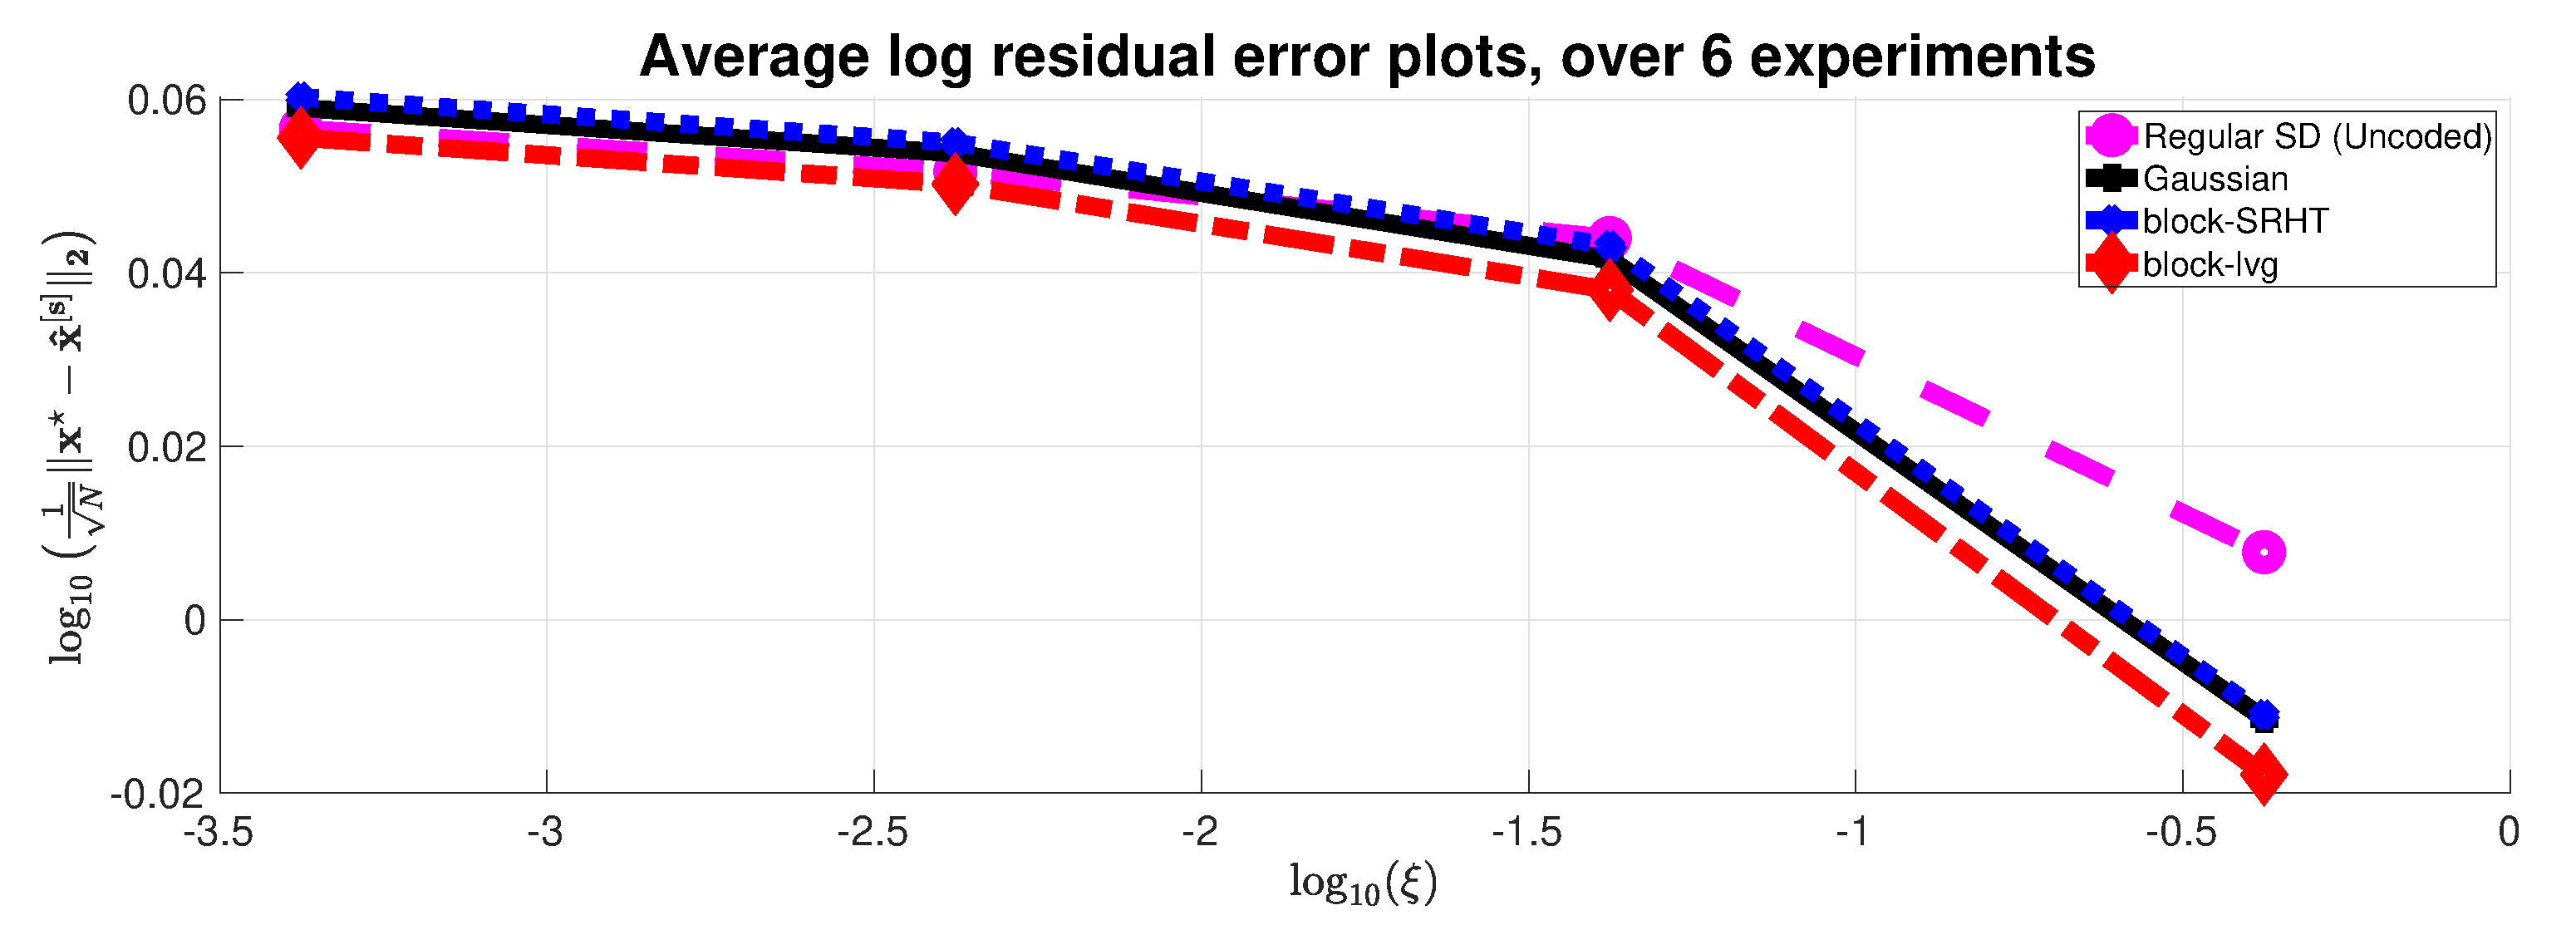
\includegraphics[scale=.22]{avg_log_over_six_exp_good-stretch.eps}
  \caption{residual error for varying $\xi_s$}
  \label{varying_its_t_distr}
\end{figure}

\begin{center}
\begin{table}[h]
\centering
\begin{tabular}{ |p{1.6cm}||p{1cm}|p{1cm}|p{1cm}|p{1cm}| }
\hline
\multicolumn{5}{|c|}{\textbf{Average $\log$ residual error $\log_{10}\big(\|\xb_{ls}^{\star}-\xbh\|_2\big/\sqrt{N}\big)$}} \\
%\multicolumn{5}{|c|}{Average $\log$ residual error $\log_{10}\left(\|\xb_{ls}^{\star}-\xbh\|_2/\sqrt{N}\right)$, over 6 experiments} \\
\hline
\hline
\textbf{$\log_{10}(\xi)$} & 0.0004 &
0.0042 & 0.0421 & 0.4207 \\
\hline
\hline
\textbf{Regular SD} & 0.0566 & 0.0517 & 0.0440 & 0.0078 \\
\hline
\textbf{Gaussian} & 0.0590 & 0.0538 & 0.0416 & -0.0114 \\
\hline
\textbf{block-SRHT} & 0.0603 & 0.0550 & 0.0431 & -0.0110 \\
\hline
\textbf{block-lvg} & 0.0556 & 0.0502 & 0.0380 & -0.0178 \\
\hline
\end{tabular}
\vspace{3mm}
\caption{Average $\log$ residual errors, for six instances of SD with fixed steps, when performing Gaussian sketching with updated sketches, iterative block-SRHT and iterative block leverage score sketching, and uncoded SD.}
\label{log_res_err_table}
\end{table}
\end{center}
%\vspace{2mm}
\vspace{-1cm}

\begin{figure}[h]
  \centering
  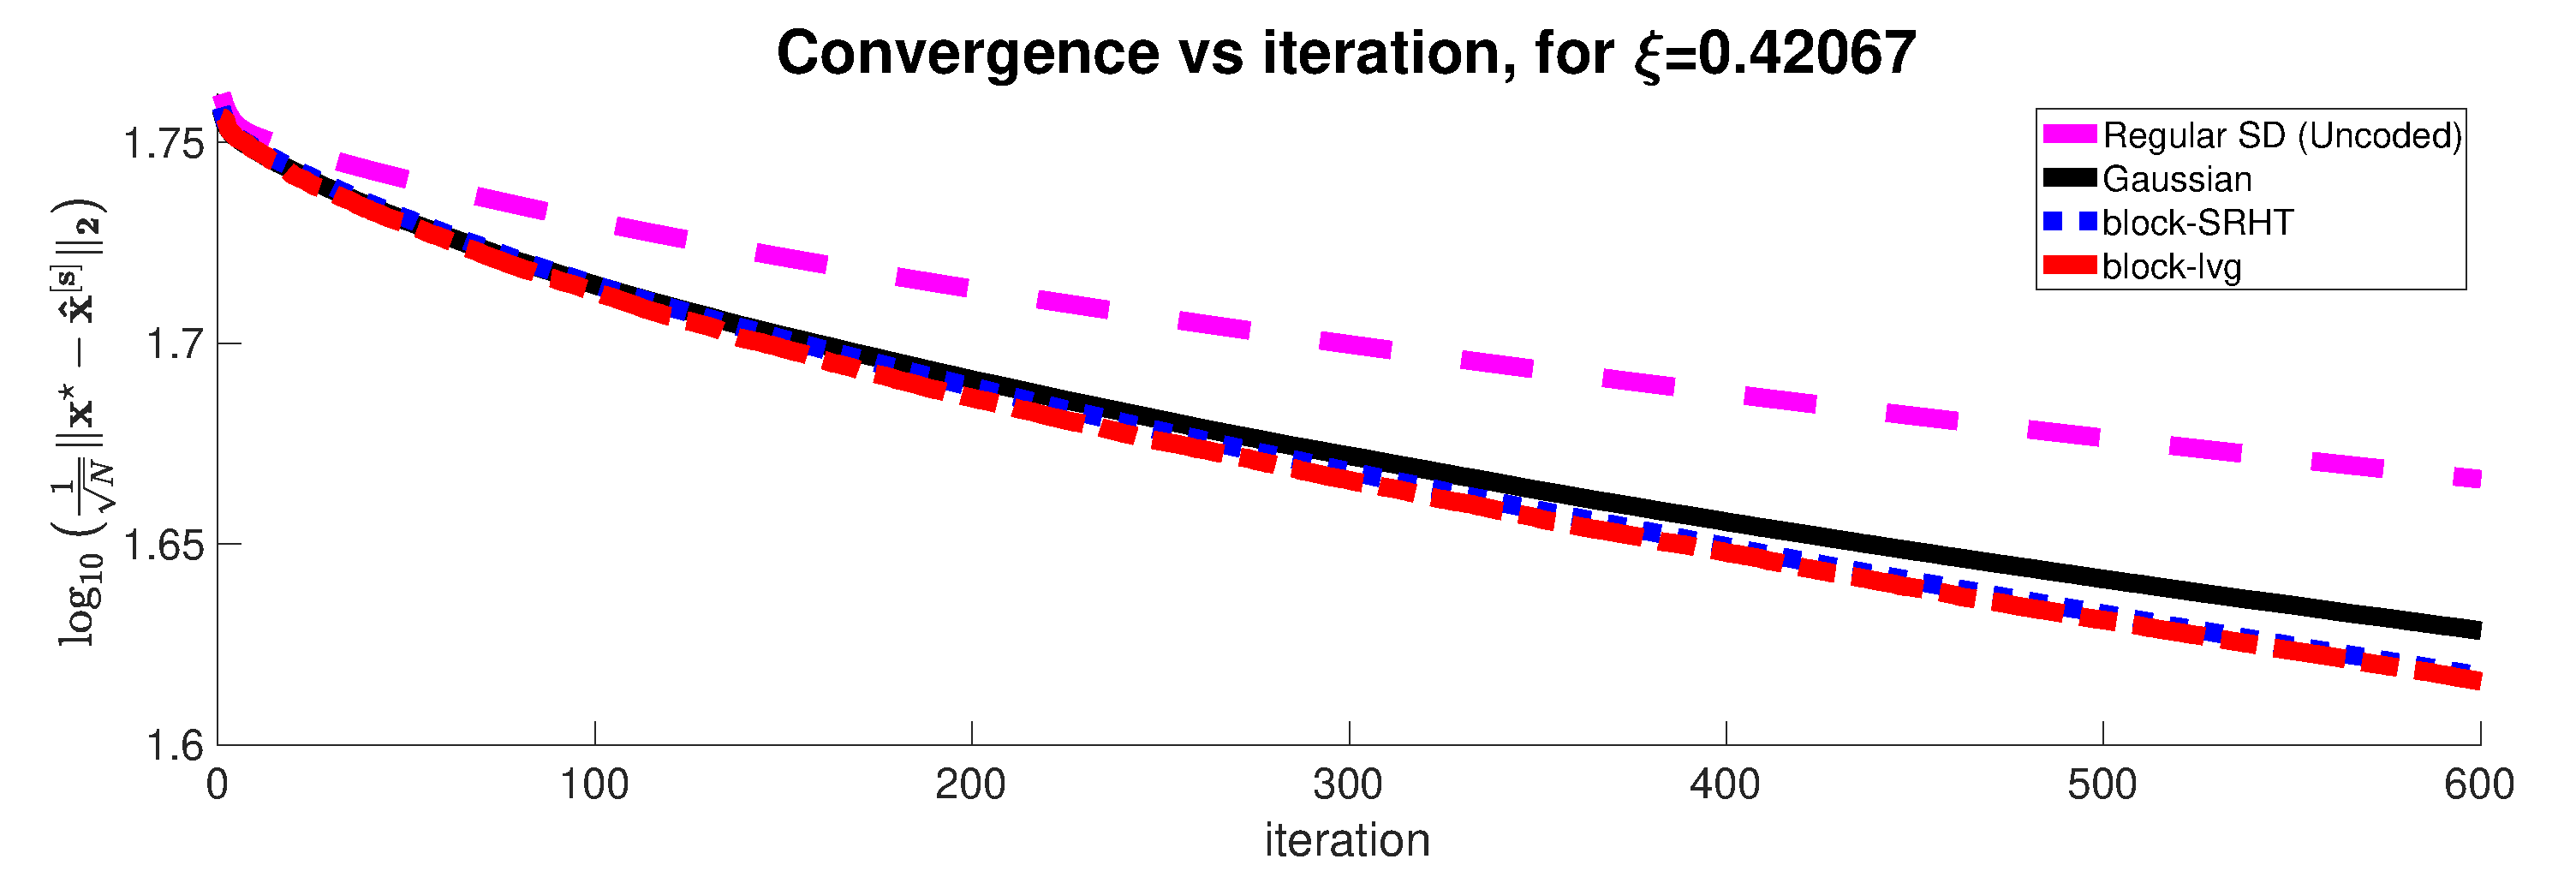
\includegraphics[scale=.22]{conv_fixed_xi_good--stretch.eps}
  \caption{$\log$ residual error convergence}
  \label{conv_fig_t_distr}
\end{figure}

\begin{comment}
\begin{figure}[h]
    \centering
    \begin{minipage}{0.5\textwidth}
        \centering
        \includegraphics[scale=.06]{comp_log_convergence_600_zoomed.png}
    \caption{residual error for varying $\xi_s$}
    \label{varying_its_t_distr}
    \end{minipage}\hfill
    \begin{minipage}{0.5\textwidth}
        \centering
        \includegraphics[scale=.06]{comp_log_convergence_600_stretch_bold.jpg}
    \caption{$\log$ residual error convergence}
    \label{conv_fig_t_distr}
    \end{minipage}
\end{figure}

\begin{figure}[h]
  \centering
  \includegraphics[scale=.2]{avg_log_over6exp--stretch.eps}
  \caption{residual error for varying $\xi_s$}
  \label{varying_its_t_distr}
\end{figure}

\begin{figure}[h]
  \centering
  \includegraphics[scale=.2]{conv_fixed_xi--stretch.eps}
  \caption{$\log$ residual error convergence}
  \label{conv_fig_t_distr}
\end{figure}
\end{comment}

We also considered the same experiment with $\Ab$ drawn from a $t$-distribution, with and optimal step-size $\xi_s^{\star} = \langle\Ab g^{[s]},\Ab\xb^{[s]}-\bb\rangle\big/\|\Ab g^{[s]}\|_2^2$ at each iteration. From Figure \ref{opt_step_t_distr}, we observe that our iterative sketching approach outperforms Gaussian sketching with updated sketches; and iterative sketching is superior to non-iterative. Furthermore, we validate Lemma \ref{SGD_nonunif_thm} and Theorem \ref{eq_opt_sols}, as our iterative sketching approach and SSD have similar convergence. Furthermore, it was observed that in some case cases when our iterative sketching method would outperform regular SD (and SSD). We also compared our method to iterative and non-iterative approaches according to the block leverage score sampling, block-SRHT, and Rademacher sketching methods, in which our corresponding approach again produced more accurate final approximations.

\begin{figure}[h]
  \centering
  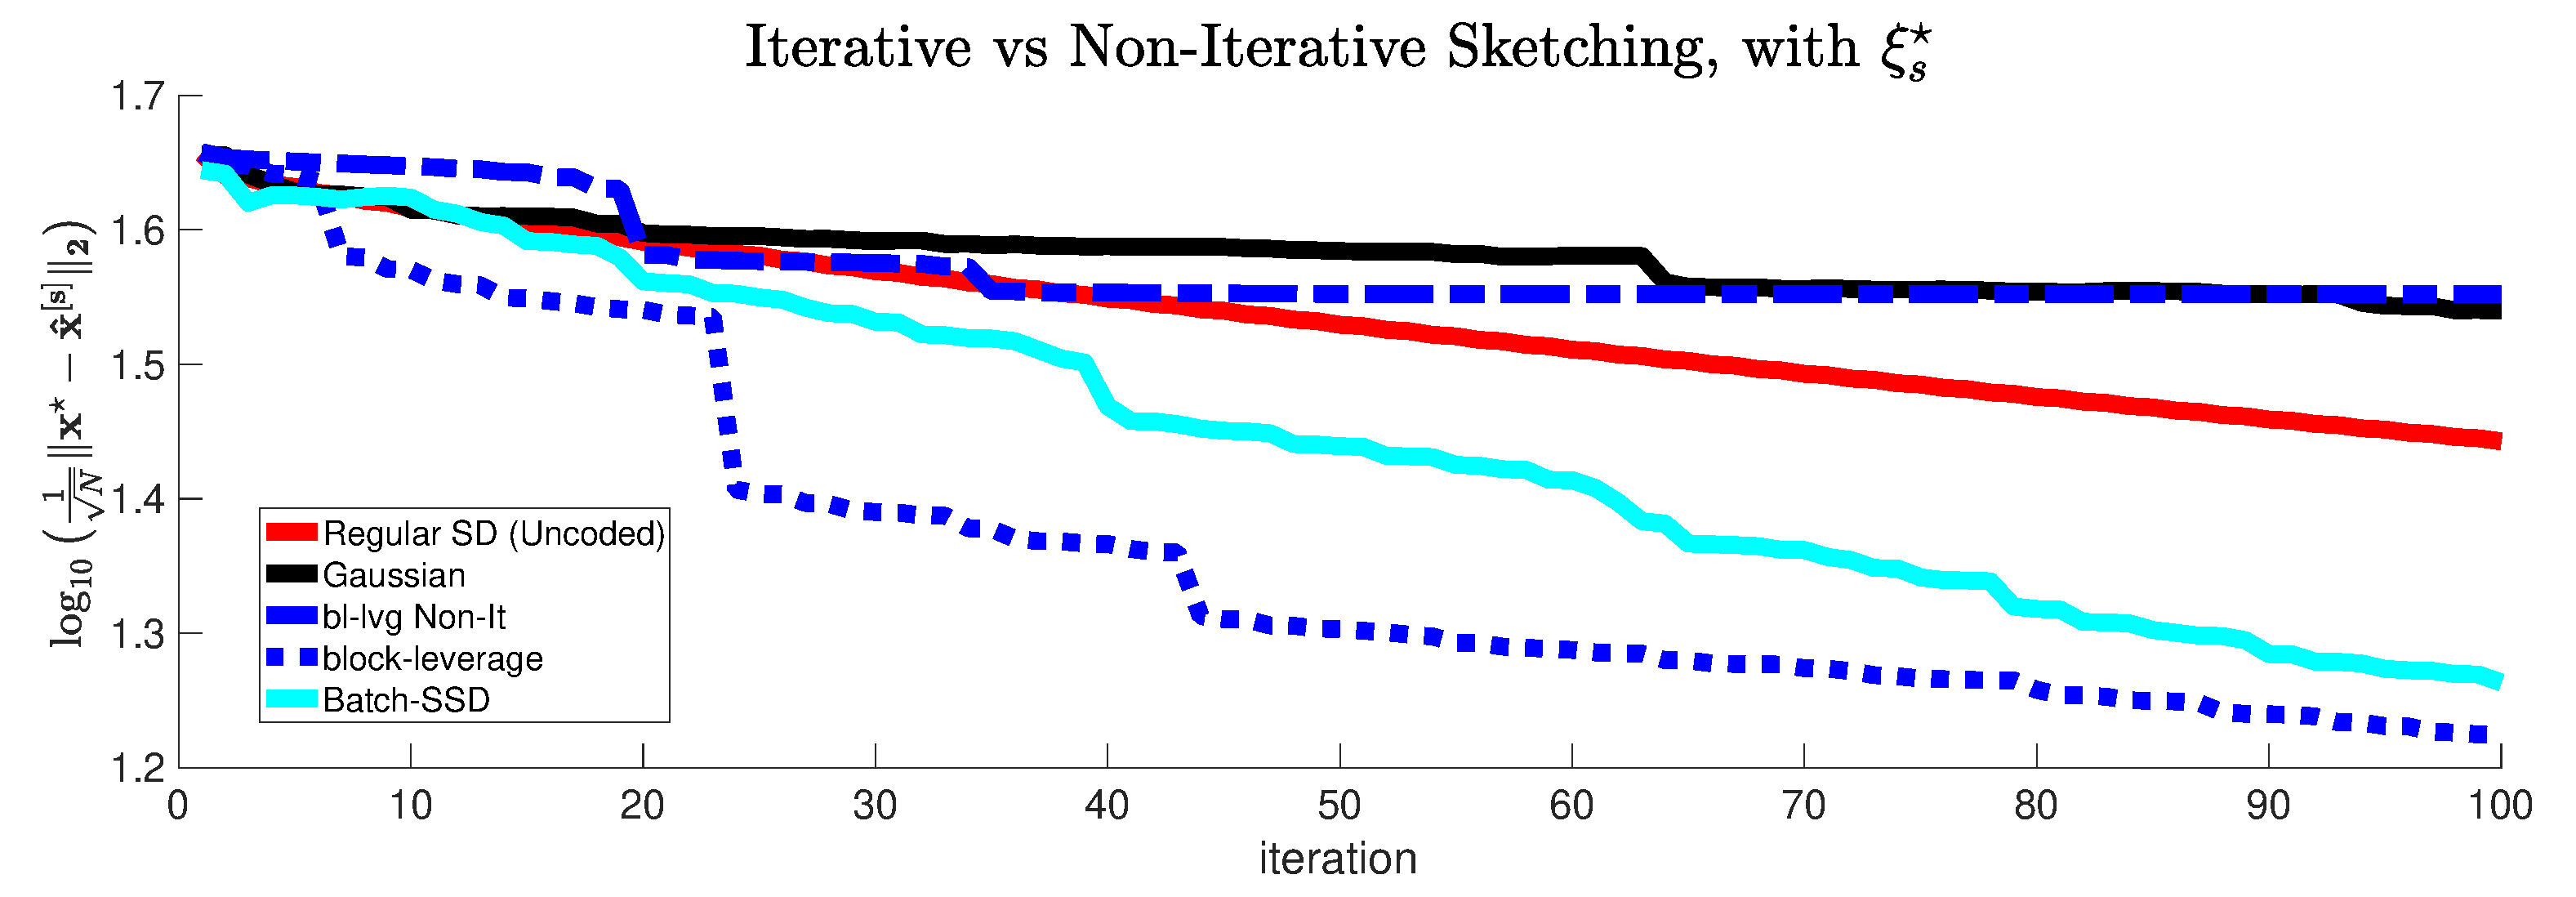
\includegraphics[scale=.2]{comp_good_NonIt_FINAL--stretch.eps}
  \caption{$\log$ convergence with $\xi_s^{\star}$}
  \label{opt_step_t_distr}
\end{figure}

\begin{comment}
\begin{figure}[h]
    \centering
    \begin{minipage}{0.5\textwidth}
        \centering
        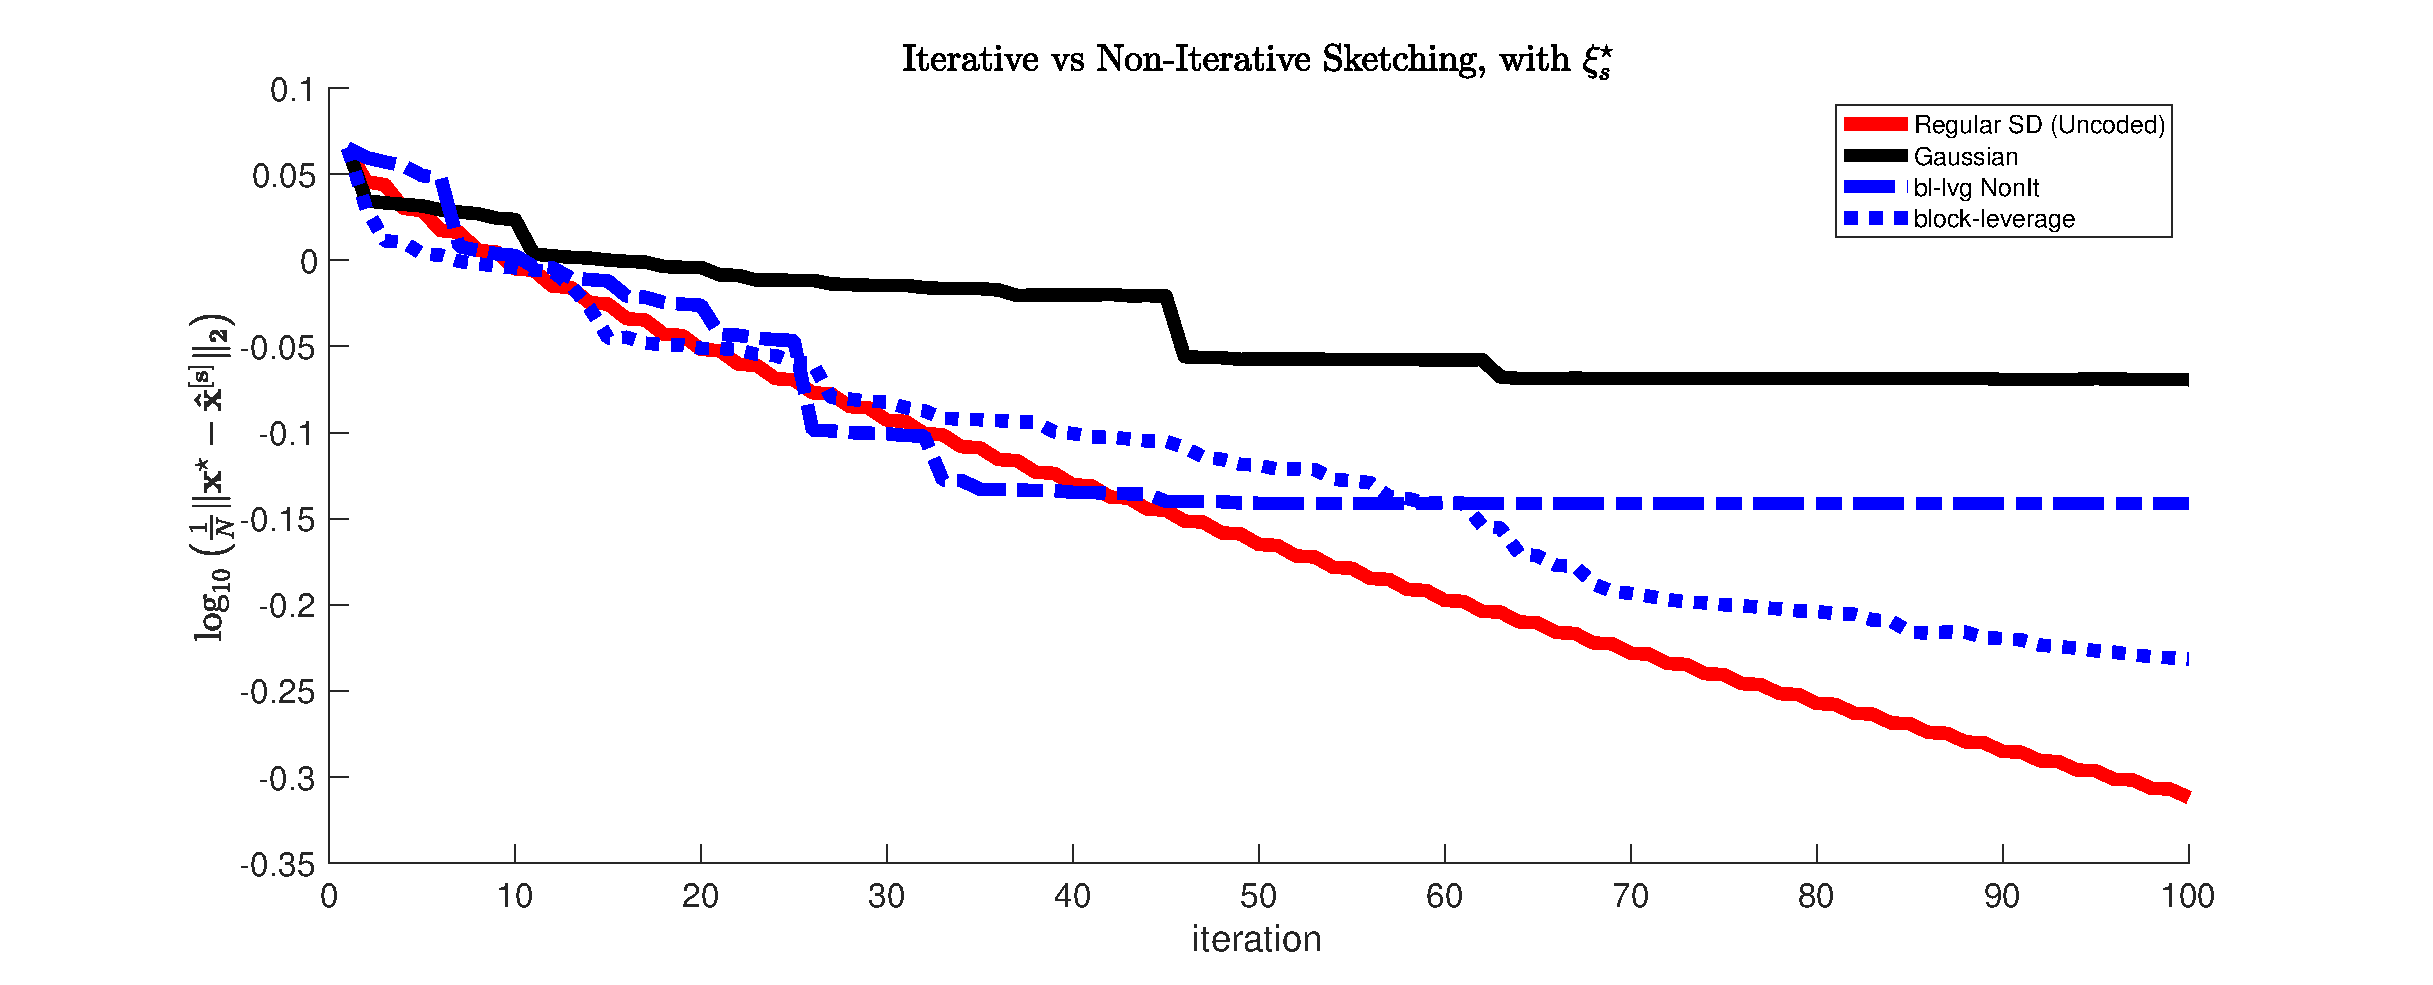
\includegraphics[scale=.2]{comp_t_distr_NonIt--stretch.eps}
        %\includegraphics[scale=.14]{noniterative_comparison_stretch.eps}
    \caption{$\log$ convergence with $\xi_s^{\star}$}
    \label{opt_step_t_distr_1}
    \end{minipage}\hfill
    \begin{minipage}{0.5\textwidth}
        \centering
        \includegraphics[scale=.2]{comp_t_distr-3--stretch.eps}
        %\includegraphics[scale=.14]{noniterative_comparison_all_10_stretch.eps}
    \caption{$\log$ convergence with $\xi_s^{\star}$}
    \label{opt_step_t_distr_2}
    \end{minipage}
\end{figure}

\begin{figure}[h]
    \centering
    \begin{minipage}{0.5\textwidth}
        \centering
        \includegraphics[scale=.2]{comp_t_distr_NonIt_5.jpg}
    \caption{$\log$ convergence with $\xi_s^{\star}$}
    \label{opt_step_t_distr_1}
    \end{minipage}\hfill
    \begin{minipage}{0.5\textwidth}
        \centering
        \includegraphics[scale=.2]{comp_t_distr_SSD_Gaussian_5.jpg}
    \caption{$\log$ convergence with $\xi_s^{\star}$}
    \label{opt_step_t_distr_2}
    \end{minipage}
\end{figure}
\end{comment}

% - - - - - - - - - - - - - - -
\begin{comment}
\subsection{Expansion Networks}

In the following experiment, we considered the empirical distribution from the server completion times taken from 500 AWS-servers \cite{BP19a}. The completion times along with the ending times $T$ we considered, are shown in Figure \ref{AWS_times}. In Table \ref{misestimations_table} we show the resulting $q(T)$, misestimation factors $\beta_{\Pib}$, metrics $\Delta_{\Pi,\Pib}$ and $d{\Pi,\Pib}$ for the corresponding methods. The resulting sketching errors $\epsilon$ are also presented in Figure \ref{embedding_error_plot}.

\begin{center}
\begin{table}[h]
\centering
\begin{tabular}{ |p{.9cm}||p{.7cm}|p{.7cm}|p{.7cm}|p{.7cm}|p{.7cm}|p{.7cm}|p{.7cm}|p{.7cm}|p{.7cm}|p{.7cm}| }
\hline
\multicolumn{11}{|c|}{Expansion Networks Misestimation Factors and Metrics} \\
\hline
\hline
{\small$t\gets T$} & 6 & 12 & 18 & 24 & 30 & 36 & 42 & 48 & 54 & 60 \\
\hline
$q(T)$ & {\small 499} & {\small 267} & {\small 262} & {\small 230} & {\small 230} & {\small 230} & {\small 230} & {\small 230} & {\small 226} & {\small 142} \\
\hline
$\Delta_{\Pi,\Pib}$ & {\footnotesize .8859} & {\footnotesize .9078} & {\footnotesize .9079} & {\footnotesize .9079} & {\footnotesize .9079} & {\footnotesize .9079} & {\footnotesize .9079} & {\footnotesize .9079} & {\footnotesize .9079} & {\footnotesize .9079} \\
\hline
$d_{\Pi,\Pib}$ & {\footnotesize .0048} & {\footnotesize .0048} & {\footnotesize .0048} & {\footnotesize .0048} & {\footnotesize .0048} & {\footnotesize .0048} & {\footnotesize .0048} & {\footnotesize .0048} & {\footnotesize .0048} & {\footnotesize .0048} \\
\hline
$\beta_{\Pib}$ & {\footnotesize .9407} & {\footnotesize .9720} & {\footnotesize .9727} & {\footnotesize .9727} & {\footnotesize .9727} & {\footnotesize .9727} & {\footnotesize .9727} & {\footnotesize .9727} & {\footnotesize .9727} & {\footnotesize .9727} \\
\hline
$\epsilon$ & {\footnotesize .1167} & {\footnotesize .1323} & {\footnotesize .1442} & {\footnotesize .1336} & {\footnotesize .1297} & {\footnotesize .1318} & {\footnotesize .1425} & {\footnotesize .1468} & {\footnotesize .1463} & {\footnotesize .1794} \\
\hline
\end{tabular}
\vspace{3mm}
\caption{Misestimations with AWS server completion times}
\label{misestimations_table}
\end{table}
\end{center}
\vspace{-1cm}

\begin{figure}[h]
    \centering
    \begin{minipage}{0.5\textwidth}
        \centering
        \includegraphics[scale=.26]{embedding_errors_1.eps}
    \caption{$\ell_2$-s.e. error $\epsilon$ with varying $t$}
    \label{embedding_error_plot}
    \end{minipage}\hfill
    \begin{minipage}{0.5\textwidth}
        \centering
        \includegraphics[scale=.24]{empirical_distr.eps}
    \caption{Empirical AWS response distribution, and selected $T$'s}
    \label{AWS_times}
    \end{minipage}
\end{figure}
\end{comment}

% - - - - - - - - - - - - - - -
\section{Conclusion and Future Work}
\label{concl_sec}

In this paper, we showed how one can exploit results from RandNLA to distributed CC, in the context of GC. By taking enough samples, or equivalently; waiting long enough, the approximation errors can be made arbitrarily small. In terms of CC, the advantages are that \textit{encodings} correspond to a scalar multiplication, and \textit{no} decoding step is required. By utilizing these techniques, we are also advantageous over other CC approximation schemes \cite{SH22,BWE19,CPH20a,CPH20c,CP18,CPE17,FD16,GW20,HYKM19,KKR19,RTTD17}; by incorporating information from our dataset into our scheme.

Our methods were validated numerically through various experiments, presented in Section \ref{exper_sec}. Further experiments were performed on various distributions for $\Ab$, in which similar results were obtained. We also considered the empirical distribution from real-server completion times taken from 500 AWS-servers \cite{BP19a}, and emulated the proposed CC scheme. In this experiment, we obtained the expected results in terms of $\ell_2$-s.e., misestimation factors $\beta_{\Pib}$, and metrics $\Delta_{\Pi,\Pib}$, $d_{\Pi,\Pib}$.

Even though we focused on leverage score sampling for linear regression, other sampling algorithms and problems could benefit by designing analogous replication schemes. One such problem is the \textit{column subset selection problem}, which can be used to compute partial $\SVD$, $\QR$ decompositions, as well as low-rank approximations \cite{Mah16}. As for the sampling technique we studied, one can judiciously define a sampling distribution to approximate solutions to such problems \cite{BMD09}, which are known to be \textsf{NP-hard} under the Unique Games Conjecture assumption \cite{Civ14}.

Furthermore, existing block sampling algorithms can also benefit from the proposed expansion networks, \textit{e.g.} $CR$-multiplication \cite{CPH20c} and $CUR$ decomposition \cite{OJXE18}. For instance, a coded matrix multiplication algorithm of minimum variance can been designed, where the sampling distribution proposed in \cite{CPH20c} is used to determine the replication numbers of the expansion network. In terms of matrix decompositions, the block leverage score algorithm of \cite{OJXE18} can be used to distributively determine an additive $\epsilon$-error decomposition of $\Ab$, in the CC setting. Another future direction is generalizing existing tensor product and factorization algorithms to block sampling, according to both approximate and exact sampling distributions, in order to make them practical for distributed environments.

% - - - - - - - - - - - - - - -
\appendices
% - - - - - - - - - - - - - - -

\section{Proofs of Subsection \ref{lvg_sec}}
%\section{Proof of Theorem \ref{subsp_emb_thm_lvg}}
\label{lvg_app}

\begin{comment}
The reduced Singular Value Decomposition of (SVD) of $\Ab$ with $\rank(\Ab)=\rho$, is a decomposition of the form
\begin{equation}
\label{SVD_decomp}
  \Ab = \overbrace{\begin{pmatrix} \Ub_k & \Ub_{\rho-k} \end{pmatrix}}^{\Ub_{\Ab}\in\R^{p\times \rho}} \overbrace{\begin{pmatrix} \Sigb_k & \bold{0} \\ \bold{0} & \Sigb_{\rho-k} \end{pmatrix}}^{\Sigb_{\Ab}\in\R^{\rho\times \rho}} \overbrace{\begin{pmatrix} \Vb_k^\top \\ \Vb_{\rho-k}^\top \end{pmatrix}}^{\Vb_{\Ab}^\top\in\R^{\rho\times q}} = \overbrace{\begin{pmatrix} \Ub_\Ab & \Ub_\Ab^{\perp} \end{pmatrix}}^{\qvec{U}\in\R^{p\times p}} \overbrace{\begin{pmatrix} \Sigb_\Ab & \bold{0} \\ \bold{0} & \bold{0} \end{pmatrix}}^{\Sigb\in\R^{p\times q}} \overbrace{\begin{pmatrix} \Vb_\Ab^\top \\ {\Vb_\Ab^{\perp}}^\top \end{pmatrix}}^{\qvec{V}^\top\in\R^{q\times q}}
\end{equation}
where the sizes of the indicated submatrices are $\Ub_k\in\R^{p\times k}$, $\Ub_{\rho-k}\in\R^{p\times(\rho-k)}$, $\Vb_k\in\R^{q\times k}$, $\Vb_{\rho-k}\in\R^{q\times(\rho-k)}$, $\Sigb_k\in\R^{k\times k}$ and $\Sigb_{\rho-k}\in\R^{(\rho-k)\times(\rho-k)}$. The column span of $\Ab$ is denoted by $\image(\Ab)$, for which $\image(\Ab)=\image(\Ub_\Ab)$. By $\Ub^{\perp}$ we denote the orthogonal complement of $\Ub$, and by $\bb^{\perp}=\Ub_\Ab^{\perp}{\Ub_\Ab^{\perp}}^\top\bb$ the part of $\bb$ sitting outside of $\image(\Ub_\Ab)$. Furthermore, $\Ub_\Ab^{\perp}{\Ub_\Ab^{\perp}}^\top=\Ib_p-\Ub_\Ab\Ub_\Ab^\top$. To simplify notation in what we will present, unless otherwise specified we will assume that $\Ab$ is full-rank. The ordered singular values of $\Ab$ are denoted by $\sigma_i(\Ab)$, and also refer to $\sigma_1$ as $\sigma_\text{max}$ and $\sigma_\rho$ as $\sigma_\text{min}$. Where clear from the context, we drop the subscript indicating the matrix whose SVD parts we are considering, and that of $k$ or $\rho-k$. The eigendecomposition of a symmetric matrix $\Mb$ is denoted by $\Qb_\Mb\bold{\Lambda}_\Mb\Qb_\Mb^\top$.
\end{comment}

In this appendix, we provide the proof of Theorem \ref{subsp_emb_thm_lvg} and Corollary \ref{sub_opt_cor}. We first recall the following matrix Chernoff bound \cite[Fact 1]{Woo14}, and prove Proposition \ref{prop_Sp_lvg}.

\begin{Thm}[Matrix Chernoff Bound, {\cite[Fact 1]{Woo14}}]
\label{matr_Chern}
  Let $\Xb_1,\cdots,\Xb_q$ be independent copies of a symmetric random matrix $\Xb\in\R^{d\times d}$, with $\E[\Xb]=0, \|\Xb\|_2\leqslant \gamma$, $\|\E[\Xb^\top\Xb]\|_2\leqslant \sigma^2$. Let $\Zb=\frac{1}{q}\sum_{i=1}^q\Xb_i$. Then $\forall\epsilon>0$:
  \begin{equation*}
  \label{matr_Chern_expr}
    \Pr\Big[\|\Zb\|_2>\epsilon\Big]\leqslant2d\cdot\exp\left(-\frac{q\epsilon^2}{\sigma^2+\gamma\epsilon/3}\right).
  \end{equation*}
\end{Thm}
\vspace{2mm}

\begin{Prop}
\label{prop_Sp_lvg}
The sketching matrix $\Sbwt$ of Algorithm \ref{alg_lvg_b} with $\Pit_i\geqslant \beta\Pi_i$ for all $i$ and $\beta\in(0,1]$, guarantees
\begin{equation}
\label{conc_lvg_b}
  \Pr\Big[\|\Ib_d-\Ub^\top\Sbwt^\top\Sbwt\Ub\|_2>\epsilon\Big] \leqslant 2d\cdot e^{-q\epsilon^2\Theta(\beta/d)}
\end{equation}
for any $\epsilon>0$, and $q=r/\tau>d/\tau$.
\end{Prop}

\begin{proof}{[Proposition \ref{prop_Sp_lvg}]}
In order to use Theorem \ref{matr_Chern}, we first need to define an appropriate symmetric random matrix $\Xb$, whose realizations $\Xb_{\{q\}}$ correspond to the sampling procedure of Algorithm \ref{alg_lvg_b}, and $\Sbwt^\top\Sbwt=\frac{1}{q}\sum_{i=1}^q\Xb_i$. The realization of the matrix random variable are
$$ \Xb_i=\Ib_d-\left(\frac{\Ub_{\left(\K_\iota^i\right)}^\top\Ub_{\left(\K_\iota^i\right)}}{\Pit_\iota}\right)=\Ib_d-\left(\frac{\sum_{l\in\K_\iota^i}\Ub_{(l)}^\top\Ub_{(l)}}{\Pit_\iota}\right) $$
where $\K_\iota^i$ indicates the $\iota^{th}$ block of $\Ab\in\R^{N\times d}$, which was sampled at trial $i$. This holds for all $\iota\in\N_K$. The expectation of the symmetric random matrix $\Xb$ is
\begin{align*}
  \E[\Xb] &\overset{\ddagger}{=} \Ib_d-\left(\sum_{j=1}^K\Pit_j\cdot\frac{\Ub_{(\K_j)}^\top\Ub_{(\K_j)}}{\Pit_j}\right)\\
  &= \Ib_d-\sum_{j=1}^K\Ub_{(\K_j)}^\top\Ub_{(\K_j)}\\
  &\overset{\sharp}{=} \Ib_d-\sum_{l=1}^N \Ub_{(l)}^\top\Ub_{(l)}\\
  &= \Ib_d-\Ib_d\\
  &=\bold{0}_{d\times d}
\end{align*}
where $\ddagger$ follows from the fact that each realization $\Xb_i$ corresponding to each $\{\K_j^i\}_{j=1}^K$ of the random matrix is sampled with probability $\Pit_j$, and in $\sharp$ we simplify the expression in terms of rank-1 outer-product matrices. Furthermore, for $\{\ellt_l\}_{l=1}^N$ the corresponding \textit{approximate} leverage scores of $\Ab$
$$ \|\Xb_i\|_2 \ \overset{\natural} {\leqslant} \ \|\Ib_d\|_2+\frac{\|\Ub_{\left(\K_\iota^i\right)}^\top\Ub_{\left(\K_\iota^i\right)}\|_2}{\Pit_\iota} \ \overset{\diamond}{\leqslant} \ 1+\frac{\sum_{l\in\K_\iota^i}\ell_l}{\left(\sum_{l\in\K_\iota^i}\ellt_l\right)\big/d} = 1+\frac{d\cdot\Pi_\iota}{\Pit_\iota} \ = \ 1+\frac{d}{\beta} $$
where in $\natural$ we use the triangle inequality on the definition of $\Xb_i$, and in $\diamond$ we use it on the sum of outer-products (the numerator of second summand).

We now upper bound the variance of the copies of $\Xb$:
\begin{align}
%\label{upp_bd_lvg_sketch}
  \left\|\E\big[\Xb_i^\top\Xb_i\big]\right\|_2 &= \left\|\E\left[\left(\Ib_d-\left(\Ub_{(\K_\iota)}^\top\Ub_{(\K_\iota)}\big/\Pit_\iota\right)\right)^\top\left(\Ib_d-\left(\Ub_{(\K_\iota)}^\top\Ub_{(\K_\iota)}\big/\Pit_i\right)\right)\right]\right\|_2 \notag\\
  &=\left\|\Ib_d-2\cdot\E\left[(\Ub_{(\K_\iota)}^\top\Ub_{(\K_\iota)}\big/\Pit_\iota\right]+\E\left[\left(\Ub_{(\K_\iota)}^\top\Ub_{(\K_\iota)}\right)^2\big/\Pit_\iota^2\right]\right\|_2\notag\\
  &=\bigg\|2\Big(\Ib_d-\overbrace{\E\left[(\Ub_{(\K_\iota)}^\top\Ub_{(\K_\iota)}\big/\Pit_\iota\right]}^{=\Ib_d}\Big)-\Ib_d+\E\left[\left(\Ub_{(\K_\iota)}^\top\Ub_{(\K_\iota)}\right)^2\big/\Pit_\iota^2\right]\bigg\|_2 \notag\\
  %&=\Big\|\E\left[\Ub_{(\K_i)}^\top\left(\Ub_{(\K_\iota)}\Ub_{(\K_i)}^\top\right)\Ub_{(\K_\iota)}\big/\Pi_i^2\right]-\Ib_d\Big\|_2 \notag\\
  &= \left\|\E\left[\left(\Ub_{(\K_\iota)}^\top\Ub_{(\K_\iota)}\right)^2\big/\Pit_\iota^2\right]-\Ib_d\right\|_2 \notag\\
  &= \left\|\left(\sum_{\iota=1}^K\Pi_\iota\cdot\left(\Ub_{(\K_\iota)}^\top\Ub_{(\K_\iota)}\right)^2\big/\Pit_\iota^2\right)-\Ib_d\right\|_2 \notag\\
  &\overset{\sharp}{\leqslant} \left\|\left(\sum_{\iota=1}^K\frac{1}{\beta}\left(\Ub_{(\K_\iota)}^\top\Ub_{(\K_\iota)}\right)^2\big/\Pit_\iota\right)-\Ib_d\right\|_2 \notag\\
  &= \left\|\left(\sum_{\iota=1}^K\frac{d}{\beta}\cdot\frac{\left(\Ub_{(\K_\iota)}^\top\Ub_{(\K_\iota)}\right)^2}{\|\Ub_{(\K_\iota)}\|_F^2}\right)-\Ib_d\right\|_2 \notag\\
  &\leqslant \left\|\left(\sum_{\iota=1}^K\frac{d}{\beta}\cdot\frac{\left(\Ub_{(\K_\iota)}^\top\Ub_{(\K_\iota)}\right)^2}{\|\Ub_{(\K_\iota)}\|_2^2}\right)-\Ib_d\right\|_2 \notag\\
  &\overset{\flat}{=} \left\|\frac{d}{\beta}\cdot\left(\sum_{\iota=1}^K\left(\Ub_{(\K_\iota)}^\top\Ub_{(\K_\iota)}\right)^2\right)-\Ib_d\right\|_2 \notag\\
  &\overset{\natural}{\leqslant} \left\|\frac{d}{\beta}\left(\sum_{\iota=1}^K\left(\Ub_{(\K_\iota)}^\top\Ub_{(\K_\iota)}\right)\left(\Ib_d-\Ub_{(\Kbar_\iota)}^\top\Ub_{(\Kbar_\iota)}\right)\right)-\Ib_d\right\|_2 \notag\\
  &= \bigg\|\frac{d}{\beta}\overbrace{\left(\sum_{\iota=1}^K\Ub_{(\K_\iota)}^\top\Ub_{(\K_\iota)}\right)}^{=\Ib_d}-\frac{d}{\beta}\left(\sum_{\iota=1}^K\left(\Ub_{(\K_\iota)}^\top\Ub_{(\K_\iota)}\right)\left(\Ub_{(\Kbar_\iota)}^\top\Ub_{(\Kbar_\iota)}\right)\right) -\Ib_d\bigg\|_2 \notag\\
  &= \bigg\|(d/\beta-1)\cdot\Ib_d-\frac{d}{\beta}\bigg(\sum_{\iota=1}^K\Ub_{(\K_\iota)}^\top\overbrace{\left(\Ub_{(\K_\iota)}\Ub_{(\Kbar_\iota)}^\top\right)}^{\bold{0}_{d\times d}}\Ub_{(\Kbar_\iota)}\bigg)\bigg\|_2 \notag\\
  &= \left\|(d/\beta-1)\cdot\Ib_d\right\|_2 \notag\\
  %&= \Big\|(d-1)\cdot\Ib_d-\Big(\sum_{\iota=1}^K\overbrace{\left(\Ub_{(\K_\iota)}^\top\Ub_{(\K_\iota)}\right)}^{\Ab_j}\overbrace{\left(\Ub_{(\K_\iota)}^\top\Ub_{(\Kbar_\iota)}\right)}^{\Ab_j^{\perp}}\Big)\Big\|_2\\
  %&\overset{\sharp}{\leqslant} \Big\|(d-1)\cdot\Ib_d\Big\|_2\\
  &= d/\beta-1 \notag
\end{align}
where in $\sharp$ we used the fact $\Pi_\iota/\Pit_\iota\leqslant1/\beta$, in $\flat$ that $\|\Ub_{(\K_\iota)}\|_2^2=1$, and in $\natural$ that $\Ub_{(\K_\iota)}^\top\Ub_{(\K_\iota)}=\Ib_d-\Ub_{(\Kbar_\iota)}^\top\Ub_{(\Kbar_\iota)}$ for each $\iota$.

According to Theorem \ref{matr_Chern}, we substitute $\gamma=1+d$ and $\sigma^2=d/\beta-1$ to get
\begin{align*}
  \frac{1}{q}\sum\limits_{i=1}^{q}\Xb_i &= \frac{1}{q}\sum\limits_{i=1}^{q}\left(\Ib_d-\frac{\Ub_{\left(\K_{j(i)}\right)}^\top\Ub_{\left(\K_{j(i)}\right)}}{\Pit_{j(i)}}\right)\\
  &= \Ib_d-\frac{1}{q}\left(\sum\limits_{i=1}^{q}\frac{\Ub_{\left(\K_{j(i)}\right)}^\top\Ub_{\left(\K_{j(i)}\right)}}{\Pit_{j(i)}}\right)\\
  &= \Ib_d-\Ub^\top\Sbwt^\top\Sbwt\Ub
\end{align*}
where the last equality follows from the definition of $\Sbwt$. Putting everything together into Theorem \ref{matr_Chern}, we get that
$$ \Pr\big[\|\Ib_d-\Ub^\top\Sbwt^\top\Sbwt\Ub\|_2>\epsilon\big]\leqslant2d\cdot e^{-q\epsilon^2\Theta(\beta/d)}. $$
\end{proof}

\begin{proof}{[Theorem \ref{subsp_emb_thm_lvg}]}
By substituting $q=\Theta\left(\frac{d}{\tau}\log{(2d/\delta)}/(\beta\epsilon^2)\right)$ in \eqref{conc_lvg_b} and taking the complementary event, we attain the desired statement.
\end{proof}

Before we prove Corollary \ref{sub_opt_cor}, we introduce the notion of \textit{block $\alpha$-balanced}, which is a generalization of \textit{$\alpha$-balanced} from \cite{PW16}. The sampling distribution $\Pi_{\{K\}}$ is said to be \textit{block $\alpha$-balanced}, if
\begin{equation}
\label{bl_alpha_bal}
  \max_{i\in\N_K}\left\{\Pi_i\right\} \leqslant \frac{\alpha}{N/\tau}=\dfrac{\alpha}{K}
\end{equation}
for some constant $\alpha$ independent of $K$ and $q$. Furthermore, in our context, if the individual leverage scores $\pi_{\{N\}}$ are $\alpha$-balanced for $\alpha$ independent of $N$ and $r$, then the block leverage scores $\Pi_{\{K\}}$ are block $\alpha$-balanced, as
\begin{equation}
\label{impl_bal_wts}  % implication balanced weights
  \max_{i\in\N_K}\left\{\Pi_i\right\} \leqslant \tau\cdot\max_{j\in\N_N}\left\{\pi_j\right\} \leqslant \tau\cdot\frac{\alpha}{N} = \frac{\alpha}{N/\tau} = \frac{\alpha}{K}\ .
\end{equation}

\begin{proof}{[Corollary \ref{sub_opt_cor}]}
From the proof of {\cite[Theorem 1]{PW16}}, we simply need to show that
$$ \big\|\E\big[\Sbwt^\top\big(\Sbwt\Sbwt^\top\big)^{-1}\Sbwt\big]\big\|_2\leqslant\eta\cdot\frac{r}{N} $$
for $\Sbwt$ a single sketch produced in Algorithm \ref{alg_lvg_b}, and an appropriate constant $\eta$ independent of $N$ and $r$. We assume that the individual leverage scores $\pi_{\{N\}}$ are $\alpha$-balanced, where $\alpha$ is a constant independent of $N$ and $r$. By \eqref{impl_bal_wts}, it follows that the block leverage scores $\Pi_{\{K\}}$ are block $\alpha$-balanced; \textit{i.e.} $\Pi_i\leqslant \Pi_K \leqslant \frac{\alpha}{K}$ for all $i\in\N_{K-1}$.

A direct computation shows that
\begin{align*}
  \big(\Sbwt\Sbwt^\top\big)^{-1} &= \Big((\Db\cdot\Omb\otimes\Ib_\tau)\cdot(\Omb^\top\cdot\Db^\top\otimes\Ib_\tau)\Big)^{-1}\\
  &= \Big(\big(\Db\cdot\Omb\cdot\Omb^\top\cdot\Db^\top\big)\otimes\Ib_\tau\Big)^{-1}\\
  &= \big(\Db\cdot\Omb\cdot\Omb^\top\cdot\Db^\top\big)^{-1}\otimes\Ib_\tau
\end{align*}
and consequently
\begin{align*}
  \Sbwt^\top\big(\Sbwt\Sbwt^\top\big)^{-1}\Sbwt &= \big(\Omb^\top\cdot\Db^\top\otimes\Ib_\tau\big) \cdot \Big(\big(\Db\cdot\Omb\cdot\Omb^\top\cdot\Db^\top\big)^{-1}\otimes\Ib_\tau\Big)\cdot(\Db\cdot\Omb\otimes\Ib_\tau) \\
  &= \Big(\Omb^\top\cdot\Db^\top \cdot \big(\Db\cdot\Omb\cdot\Omb^\top\cdot\Db^\top\big)^{-1}\otimes\Ib_\tau\Big)\cdot(\Db\cdot\Omb\otimes\Ib_\tau) \\
  &= \underbrace{\Big(\Omb^\top\cdot\Db^\top \cdot \big(\Db\cdot\Omb\cdot\Omb^\top\cdot\Db^\top\big)^{-1}\cdot\Db\cdot\Omb\Big)}_{\coloneqq Z\in\R_{\geqslant0}^{K\times K}}\otimes\Ib_\tau \\
\end{align*}
where $Z=\sum_{\iota=1}^qZ_\iota$, for $\{Z_\iota\}_{\iota=1}^q$ rank-1 outer-product matrices of size $K\times K$ corresponding to each sampling trial, through $\Omb$. For each sampling trial, we know that the $i^{th}$ block is sampled with probability $\Pi_i$. Furthermore, if the $i^{th}$ block is sampled at iteration $\iota$, it follows that
\begin{align*}
  Z_\iota &= \eb_i\cdot\sqrt{\frac{1}{q\Pi_i}}\cdot\left(\eb_i^\top\cdot\left(\sqrt{\frac{1}{q\Pi_i}}\right)^2\cdot\eb_i\right)^{-1}\cdot\sqrt{\frac{1}{q\Pi_i}}\cdot\eb_i^\top \\
  &= \eb_i\cdot\sqrt{\frac{1}{q\Pi_i}}\cdot\left(\sqrt{q\Pi_i}\right)^2\cdot\sqrt{\frac{1}{q\Pi_i}}\cdot\eb_i^\top \\
  &= \eb_i\cdot\eb_i^\top
\end{align*}
hence
\begin{equation*}
  \E\left[\Sbwt^\top\big(\Sbwt\Sbwt^\top\big)^{-1}\Sbwt\right] = \E_\Omb\left[\sum_{j=1}^K\eb_j\cdot\eb_j^\top\right]\otimes\Ib_\tau = \left(\sum_{j=1}^K\E_\Omb\left[\eb_j\cdot\eb_j^\top\right]\right)\otimes\Ib_\tau = \Qb\otimes\Ib_\tau
\end{equation*}
where $\Qb=\diag\big(\{h_j\}_{j=1}^q\big)$, for $h_i=1-(1-\Pi_i)^q$ the probability that the $i^{th}$ block was sampled at least once. Since we assume that the blocks $\Ab_{\{K\}}$ are indexed in ascending order according their block leverage scores; \textit{i.e.} $\Pi_i\leqslant\Pi_{i+1}$ for all $i\in\N_{K-1}$, it follows that $h_i\leqslant h_K$ for all $i$; thus%$h_i\coloneqq\Pr\big[\text{block $i$ was sampled}\big]=1-(1-\Pi_i)^q$
\begin{equation*}
  \E\left[\Sbwt^\top\big(\Sbwt\Sbwt^\top\big)^{-1}\Sbwt\right] = \diag\left(\{h_j\}_{j=1}^q\right)\otimes\Ib_\tau \preceq h_K\cdot\Ib_N = \big(1-(1-\Pi_K)^q\big)\cdot\Ib_N \preceq q\Pi_K\cdot\Ib_N\ .
\end{equation*}
Consequently, since $\Pi_{\{K\}}$ are block $\alpha$-balanced; we have
\begin{equation*}
  \left\|\E\left[\Sbwt^\top\big(\Sbwt\Sbwt^\top\big)^{-1}\Sbwt\right]\right\|_2 \leqslant q\cdot\Pi_K \leqslant \alpha\cdot\frac{q}{K} = \alpha\cdot\frac{r}{N} .
\end{equation*}
This completes the proof, as we can take $\eta=\alpha$.
\end{proof}

% - - - - - - - - - - - - - - -
\section{Concrete Example of Induced Sketching}
\label{app_example}

In this appendix, we give a simple demonstration of the induced sketching matrices, through our proposed GC approach. For simplicity, we will consider exact sampling, with $\Pi_{\{K\}}=\{3/20,3/20,4/20,5/20,5/20\}$ for $K=5$, an arbitrary large block size of $\tau$, and $m=20$. The optimal replication numbers resulting from this distribution are $r^{\star}_{\{K\}}=\{3,3,4,5,5\}$, hence $m=R$. In order to obtain a reduced dimension $r$ which is 60\% of the original $N$, we carry out $q=3$ sampling trials at each iteration.

Let the resulting index multisets corresponding to the encoded pairs $(\At_j,\bt_j)$ of the first four iterations; along with the resulting estimated gradients, be:
\begin{enumerate}
  \item $\Scal^{[1]}=\{1,4,5\} \ \ \implies \ \ \gh^{[1]}=\nabla_\xb L_\Sb\left(\Sbwt_{[1]},\Ab,\bb;\xb^{[1]}\right)=\gh_1^{[1]}+\gh_4^{[1]}+\gh_5^{[1]}$
  \item $\Scal^{[2]}=\{3,5,5\} \ \ \implies \ \ \gh^{[2]}=\nabla_\xb L_\Sb\left(\Sbwt_{[2]},\Ab,\bb;\xb^{[2]}\right)=\gh_3^{[2]}+\gh_5^{[2]}+\gh_5^{[2]}$
  \item $\Scal^{[3]}=\{2,4,5\} \ \ \implies \ \ \gh^{[3]}=\nabla_\xb L_\Sb\left(\Sbwt_{[3]},\Ab,\bb;\xb^{[3]}\right)=\gh_2^{[3]}+\gh_4^{[3]}+\gh_5^{[3]}$
  \item $\Scal^{[4]}=\{4,1,4\} \ \ \implies \ \ \gh^{[4]}=\nabla_\xb L_\Sb\left(\Sbwt_{[4]},\Ab,\bb;\xb^{[4]}\right)=\gh_4^{[4]}+\gh_1^{[4]}+\gh_4^{[4]}\ $.
\end{enumerate}
Then, the corresponding \textit{induced} block leverage score sketching matrices of Algorithm \ref{alg_lvg_b}, are:
\begin{align*}
  \Sbwt_{[1]} &= \begin{pmatrix} 1/\sqrt{3\Pi_1} & 0 & 0 & 0 & 0 \\ 0 & 0 & 0 & 1/\sqrt{3\Pi_4} & 0 \\ 0 & 0 & 0 & 0 & 1/\sqrt{3\Pi_5} \end{pmatrix} \otimes\Ib_\tau \qquad \qquad \Sbwt_{[2]} = \begin{pmatrix} 0 & 0 & 1/\sqrt{3\Pi_3} & 0 & 0 \\ 0 & 0 & 0 & 0 & 1/\sqrt{3\Pi_5} \\ 0 & 0 & 0 & 0 & 1/\sqrt{3\Pi_5} \end{pmatrix}\otimes\Ib_\tau\\
  \Sbwt_{[3]} &= \begin{pmatrix} 0 & 1/\sqrt{3\Pi_2} & 0 & 0 & 0 \\ 0 & 0 & 0 & 1/\sqrt{3\Pi_4} & 0 \\ 0 & 0 & 0 & 0 & 1/\sqrt{3\Pi_5} \end{pmatrix}\otimes\Ib_\tau \qquad \qquad \Sbwt_{[4]} = \begin{pmatrix} 0 & 0 & 0 & 1/\sqrt{3\Pi_4} & 0 \\ 1/\sqrt{3\Pi_1} & 0 & 0 & 0 & 0 \\  0 & 0 & 0 & 1/\sqrt{3\Pi_4} & 0 \end{pmatrix}\otimes\Ib_\tau
\end{align*}
each of which are of size $(3\tau)\times(5\tau)$.

% - - - - - - - - - - - - - - -
\section{Comparison to the block-SRHT}
%\section{Flattening of Sampling Distribution}
\label{comp_SRHT_app}

An alternative view point is that the matrix $\Ubt_{\mathrm{exp}}\coloneqq\PsiB\cdot(\Sigb\Vb^\top)^{-1}$ has uniform Frobenius block scores, which further justifies the proposed GC approach for homogeneous servers. This resembles the main idea behind the SRHT \cite{AC06,DMMS11} and different variants known as \textit{block-SRHT} \cite{CMPH22,BBGL22}, where a random projection is applied to the data matrix to ``flatten'' its leverage scores, \textit{i.e.} make them close to uniform. These two techniques for flattening the corresponding block scores are vastly different, and the proximity of the corresponding block scores are measured and quantified differently. In contrast to the block-SRHT, the quality of the approximation in our case depends on the misestimation factor $\beta_{\Pit}$; and is not quantified probabilistically.% is the quantification of their proximity of the resulting distributions to the uniform distribution.

We note that since $\PsiB$ has repeated blocks from the expansion, the scores we consider in Lemma \ref{Lemma_flat} are not the block leverage scores of $\PsiB$. The Frobenius block scores of $\Ubt_{\mathrm{exp}}$, are in fact the corresponding block leverage scores of $\Abt$, which are replicated in the expansion. Moreover, note that the closer $\beta_{\Pit}$ is to $1$, the closer the sampling distribution according to the Frobenius block scores of $\Ubt_{\mathrm{exp}}$; which we denote by $\Qt_{\{R\}}$, is to being exactly uniform. We denote the uniform sampling distribution by $\Uu_{\{R\}}$.

\begin{Lemma}
\label{Lemma_flat}
When $\Pit_{\{K\}}=\Pi_{\{K\}}$, the sampling distribution $\Qt_{\{R\}}$ is uniform. When $\Pit_\iota\geqslant\beta_{\Pit}\Pi_\iota$ for $\beta_{\Pit}=\min_{i\in\N_K}\{\Pi_i/\Pit_i\}\in(0,1)$ and all $\iota\in\N_K$, the resulting distribution $\Qt_{\{R\}}$ is approximately uniform, and satisfies  $d_{\Uu,\Qt}\leqslant1\big/(R\beta_{\Pit})$.
%Denote the sampling distribution according to the Frobenius block scores of $\Ubt_{\mathrm{exp}}$ by $\Qt_{\{K\}}$. When $\Pit_{\{K\}}=\Pi_{\{K\}}$, this distribution is uniform (denoted $\Uu_{\{K\}}$). When $\Pit_\iota\geqslant\beta_{\Pit}\Pi_\iota$ for $\beta_{\Pit}=\min_{i\in\N_K}\{\Pi_i/\Pit_i\}\in(0,1)$, the resulting $\Qt_{\{K\}}$ is approximately uniform, and satisfies  $d_{\Uu,\Qt}\leqslant1/(K\beta_{\Pit})$.%$\sum_{\iota=1}^R\|\Qt_i-1/R\|_1\leqslant1/\beta_{\Pit}$.
%The sampling distribution according to the Frobenius block scores of $\PsiB\cdot(\Sigb\Vb^\top)^{-1}$ is uniform up to a factor of $1/\beta_{\Pit}$.\footnote{Since $\PsiB$ has repeated blocks from the expansion, the scores we consider here are not the block leverage scores of $\PsiB$. The Frobenius block scores of $\PsiB\cdot(\Sigb\Vb^\top)^{-1}$, are in fact the corresponding block leverage scores of $\Abt$, which are replicated in the expansion.} If $\Pit_{\{K\}}=\Pi_{\{K\}}$, this distribution is uniform.
\end{Lemma}

\begin{proof}
Let $\Ub=\Big[\Ub_1^\top \ \cdots \ \Ub_K^\top\Big]^\top$ denote the corresponding blocks of $\Ub$ according the partitioning of $\D$. Without loss of generality, assume that the data points within each partition are consecutive rows of $\Ab$, and $\Ub_\iota\in\R^{\tau\times d}$ for all $\iota\in\N_K$.

From \eqref{expansion_matrix} and \eqref{scalar_enc_matrix}, it follows that
\begin{align*}
  \PsiB &= \Ebwt\cdot\Abt = \left(\Eb\otimes\Ib_\tau\right)\cdot\left(\Gb\cdot\Ub\Sigb\Vb^\top\right) \\
  &= \left(\Eb\otimes\Ib_\tau\right) \cdot \left[\Ub_1^\top\big/\sqrt{q\Pit_1} \ \cdots \ \Ub_K^\top\big/\sqrt{q\Pit_K}\right]^\top \cdot \Sigb\Vb^\top \\
  &\eqqcolon \left(\Eb\otimes\Ib_\tau\right) \cdot \left[\Ubt_1^\top \ \cdots \ \Ubt_K^\top\right]^\top \cdot \Sigb\Vb^\top \\
  &\eqqcolon \overbrace{\bigg[ \underbrace{\Ubt_1^\top \ \cdots \ \Ubt_1^\top}_{r_1} \ \underbrace{\Ubt_2^\top \ \cdots \ \Ubt_2^\top}_{r_2} \ \cdots \ \underbrace{\Ubt_K^\top \ \cdots \ \Ubt_K^\top}_{r_K} \bigg]^\top}^{\Ubt_{\mathrm{exp}}\in\R^{R\tau\times d}} \cdot \Sigb\Vb^\top .
\end{align*}
Note that $\Ubt_{\mathrm{exp}}\Sigb\Vb^\top$ is not the $\SVD$ of $\PsiB$. For the normalizing factor of $\frac{q}{Rd}$:
$$ \Qt_\iota = \frac{q}{Rd}\cdot\|\Ubt\|_F^2 = \frac{q}{Rd}\cdot\frac{\|\Ub_\iota\|_F^2}{q\Pit_\iota} = \frac{\Pi_\iota}{R\Pit_\iota} \leqslant \frac{1}{R\beta_{\Pit}} \quad \implies \quad \sum_{i=1}^R\big|\Qt_i-1/R\big|\overset{\triangle}{\leqslant} \frac{R}{R\beta_{\Pit}} = \frac{1}{\beta_{\Pit}}\ , $$
where $\triangle$ follows from the fact that $\big|\Qt_i-1/R\big|\leqslant1\big/\big(R\beta_{\Pit}\big)$ for each $i\in\N_R$. After normalizing by $1/R$ according to the distortion metric, we deduce that $d_{\Uu,\Qt}\leqslant1\big/\big(R\beta_{\Pit}\big)$.
\begin{comment}
where $\triangle$ follows from the triangle inequality, as $\big(\Qt_i-1/R\big)\leqslant1\big/\big(R\beta_{\Pit}\big)$ for each $i\in\N_R$. After normalizing by $1/K$ according to the distortion metric, we get that $d_{\Uu,\Qt}\leqslant1\big/\big(K\beta_{\Pit}\big)$.
\begin{equation*}
\label{normalize_Q_distr}
  \Qt_\iota = \frac{q}{Rd}\cdot\|\Ubt\|_F^2 = \frac{q}{Rd}\cdot\frac{\|\Ub_\iota\|_F^2}{q\Pit_\iota} = \frac{\Pi_\iota}{R\Pit_\iota} \leqslant \frac{1}{R\beta_{\Pit}} \quad \implies \quad \Qt_\iota-\frac{1}{R} \leqslant \frac{1}{R\beta_{\Pit}}-\frac{1}{R} = \frac{1}{R}\cdot\left(\frac{1}{\beta_{\Pit}}-1\right) \leqslant \frac{1}{R}
\end{equation*}
\end{comment}

In the case where $\Pit_{\{K\}}=\Pi_{\{K\}}$, we have
$$ \Qt_\iota = \frac{q}{Rd}\cdot\|\Ubt_\iota\|_F^2 = \frac{q}{Rd}\cdot\frac{\|\Ub_\iota\|_F^2}{q\Pi_\iota} = \frac{\Pi_\iota}{R\Pi_\iota} = \frac{1}{R} $$
for all $\iota\in\N_K$, thus $\Qt_{\{K\}}=\Uu_{\{K\}}$.
\end{proof}
%The sampling matrix $\Ombwt^{[s]}$ (and the updated index set $\I^{[s]}$ of non-straggling servers) is what determines the stochasticity of our procedure and GC scheme, and what implies iterative sketching.

Finally, in Proposition \ref{comparison_two_embds} we show when the block leverage score sampling sketch of Algorithm \ref{alg_lvg_b} and the block-SRHT of \cite{CMPH22} have the same $\ell_2$-s.e. guarantee. We first recall the corresponding result to Theorem \ref{subsp_emb_thm_lvg}, of the block-SRHT.

%\begin{Thm}[$\ell_2$-s.e. of the block-SRHT, \cite{CMPH22}]
\begin{Thm}[{\cite[Theorem 7]{CMPH22}}]
\label{subsp_emb_thm_SRHT}
The block-SRHT $\Sb_{\Hbh}$ is a $\ell_2$-s.e. of $\Ab$. For $\delta>0$ and $q=\Theta\big(\frac{d}{\tau}\log(Nd/\delta)\cdot\log(2d/\delta)/\epsilon^2\big)$:
$$ \Pr\left[\|\Ib_d-\Ub^\top\Sb_{\Hbh}^\top\Sb_{\Hbh} \Ub\|_2\leqslant\epsilon\right]\geqslant 1-\delta \ . $$
\end{Thm}

\begin{Prop}
\label{comparison_two_embds}
Let $\beta=1$. For $\delta=e^{\Theta(1)}/(Nd)$, the sketches of Algorithm \ref{alg_lvg_b} and the block-SRHT of \cite{CMPH22} achieve the same asymptotic $\ell_2$-s.e. guarantee, for the same number of sampling trials $q$.
\end{Prop}

\begin{proof}
For $\delta=e^{\Theta(1)}/(Nd)$, the two sketching methods have the same $q$; and both satisfy the $\ell_2$-s.e. property with error probability $1-\delta$.% \eqref{eq_form}.
%For $\delta=e^{\Theta(1)}/(Nd)$, the two sketching methods have the same $q$ for the same error probability $1-\delta$.
\end{proof}

\begin{comment}
\begin{Prop}
\label{comparison_two_embds}
Let $\beta=1$. For $\delta=e^{\Theta(1)}$, the sketches of Algorithm \ref{alg_lvg_b} and the block-SRHT from \cite{CMPH22} achieve the same guarantees for the same number of sampling trials $q$, when $N=\omega(2d)$.
\end{Prop}

\begin{proof}{[Proposition \ref{comparison_two_embds}]}
Let $\chi=\log(2d)$, and by assumption $\delta=e^{\Theta(1)}/2$. By equating the number of sampling trials from Theorems \ref{subsp_emb_thm_lvg} and \ref{subsp_emb_thm_SRHT}, we get
\begin{align*}
  0 &= \log\left(\frac{Nd}{\delta}\right)\cdot\log\left(\frac{Nd}{\delta}\right)\\
  &= \log\left(\frac{2Nd}{e^{\Theta(1)}}\right)\cdot\log\left(\frac{2d}{e^{\Theta(1)}}\right)\\
  &= \Big(\log(2Nd)-\log(e^{\Theta(1)})\Big)\cdot\Big(\log(2d)-\log(e^{\Theta(1)})\Big)\\
  &= \Big(\chi+\log N-{\Theta(1)}\Big)\cdot\Big(\chi-\Theta(1)\Big)\\
  &= \chi^2+\chi\cdot\big(\log N - 2\Theta(1)\big)+\Theta(1)\cdot\big(\Theta(1) - \log N\big)
\end{align*}
By solving this quadratic equation with respect to $\chi$, we get that
\begin{align*}
  \chi &= \frac{1}{2}\sqrt{\log(N)^2-2\log(N)+4\Theta(1)+1} + \log(N)-\Theta(1)-1 = o(\log N)\ .
\end{align*}
therefore $\omega(\log(2d))=\log N$. Since $\log$ is monotonic, we conclude that $N=\omega(2d)$.
\end{proof}
\end{comment}

% - - - - - - - - - - - - - - -
\section{Contraction Rate of Block Leverage Score Sampling}
\label{cont_rate_app}

In this appendix we quantify the contraction rate of our method on the error term $\xb^{[s]}-\xb^\star$, which further characterizes the convergence of SD after applying our method. The contraction rate is compared to that of regular SD.

Recall that the contraction rate of an iterative process given by a function $h(x^{[s]})$ is the constant $\gamma\in(0,1)$ for which at each iteration we are guaranteed that $h(x^{[s+1]})\leqslant \gamma\cdot h(x^{[s]})$, therefore $h(x^{[s]})\leqslant \gamma_s\cdot h(x^{[0]})$. Let $\xi$ be a fixed step-size, $\Sbwt_{[s]}$ the induced sketching matrix of Algorithm \ref{alg_lvg_b} at iteration $s$, and define $\Bb_{SD}=\left(\Ib_d-2\xi\cdot\Ab^\top\Ab\right)$ and $\Bb_s=\left(\Ib_d-2\xi\cdot\Ab^\top\Sbwt_{[s]}^\top\Sbwt_{[s]}\Ab\right)$. We note that the contraction rates could be further improved if one also incorporates an optimal step-size. It is also worth noting that when weighting from Appendix \ref{weighting_sec} is introduced, we have the same contraction rate and straggler ratio.

\begin{Lemma}
\label{lem_exp_StS}
For $\Sbwt$ the sketching matrix of Algorithm \ref{alg_lvg_b}, we have $\E\left[\Sbwt^\top\Sbwt\right]=\Ib_N$.
\end{Lemma}

\begin{proof}
Similar to the proof of Proposition \ref{prop_Sp_lvg}, we define a symmetric random matrix $\Yb$, whose realizations correspond to the sampled and rescaled submatrices of Algorithm 1. The realizations are
$$ \Yb_i = \frac{\Ib_{(\K_\iota^i)}^\top\Ib_{(\K_\iota^i)}}{q\Pit_\iota} = \frac{\sum_{l\in\K_\iota^i}\eb_l\eb_l^\top}{q\Pit_\iota}\ . $$
After $q$ sampling trials, we have $\Sbwt^\top\Sbwt=\sum_{i=1}^q\Yb_i$. It follows that
$$ \E\left[\Sbwt^\top\Sbwt\right] = \E\left[\sum_{i=i}^q\Yb_i\right] = \sum_{i=1}^q\cdot\E\left[\Yb_i\right] = q\cdot \left(\sum_{j=1}^K\Pit_j\cdot\frac{\Ib_{(\K_j)}^\top\Ib_{(\K_j)}}{q\Pit_j}\right) = \sum_{j=1}^K\Ib_{(\K_j)}^\top\Ib_{(\K_j)} = \sum_{l=1}^N\eb_{(l)}\eb_{(l)}^\top = \Ib_N\ . $$
\end{proof}

\begin{Thm}
\label{contr_rate_thm}
The contraction rate of our GC approach through the expected sketch $\Sbwt_{[s]}$ at each iteration, is equal to the contraction rate of regular SD. Specifically, for $e_s\coloneqq\xb^{[s]}-\xb^\star$ the error at iteration $s$ and $\gamma_{SD}=\lambda_1(\Bb_{SD})$ the contraction rate of regular SD, we have $\big\|\E[e_{s+1}]\big\|_2\leqslant\gamma_{SD}\cdot\|e_s\|_2$.
\end{Thm}

\begin{proof}
For a fixed step-size $2\xi$, our SD parameter update at iteration $s+1$ is
$$ \xb^{[s+1]}\gets\xb^{[s]}-2\xi\cdot\Ab^\top\Sbwt_{[s]}^\top\Sbwt_{[s]}\left(\Ab\xb^{[s]}-\bb\right)\ , $$
where for regular SD we have $\Sbwt_{[s]}\gets\Ib_N$. At iteration $s+1$, the error $e_s$ of the previous iteration is not random, hence $\E[e_s]=e_s$. By substituting the expression of $\Bb_s$, it follows that% The error at iteration $s$ is $e_s\coloneqq\xb^{[s]}-\xb^\star$, and let $\Bb_s=(\Ib_d-2\xi\Ab^\top\Sbwt_{[s]}^\top\Sbwt_{[s]}\Ab)$. It follows that
\begin{align}
  e_{s+1} &= \xb^{[s+1]}-\xb^\star \notag\\
  &= \left(\xb^{[s]}-2\xi\Ab^\top\Sbwt_{[s]}^\top\Sbwt_{[s]}\left(\Ab\xb^{[s]}-\bb\right)\right)-\xb^\star \notag\\
  &= \xb^{[s]}-2\xi\Ab^\top\Sbwt_{[s]}^\top\Sbwt_{[s]}\Ab\xb^{[s]}+2\xi\Ab^\top\Sbwt_{[s]}^\top\Sbwt_{[s]}\bb-\xb^\star \notag\\
  &= \Bb_s\xb^{[s]}-\left(\xb^\star-2\xi\Ab^\top\Sbwt_{[s]}^\top\Sbwt_{[s]}\bb\right) \notag\\
  &= \Bb_s\xb^{[s]}-\left(\xb^\star-2\xi\Ab^\top\Sbwt_{[s]}^\top\Sbwt_{[s]}\left(\Ab\xb^\star+\bb^\perp\right)\right) \notag\\
  &= \Bb_s\left(\xb^{[s]}-\xb^\star\right) - 2\xi\Ab^\top\Sbwt_{[s]}^\top\Sbwt_{[s]}\bb^\perp \notag\\
  &= \Bb_s e_s - 2\xi\Ab^\top\Sbwt_{[s]}^\top\Sbwt_{[s]}\bb^\perp \label{contr_rate_Bs}
\end{align}
and by Lemma \ref{lem_exp_StS}%, we get that
\begin{equation}
\label{exp_null_term}
  \E\left[2\xi\Ab^\top\Sbwt_{[s]}^\top\Sbwt_{[s]}\bb^\perp\right] = 2\xi\Ab^\top\E\left[\Sbwt_{[s]}^\top\Sbwt_{[s]}\right]\bb^\perp = 2\xi\Ab^\top\bb^\perp = \bold{0}_{d\times 1}
\end{equation}
as $\bb^\perp$ lies in the kernel of $\Ab^\top$, and
\begin{equation}
\label{exp_Bs_term}
  \E\left[\Bb_s\right] = \Ib_d-2\xi\Ab^\top\E\left[\Sbwt_{[s]}^\top\Sbwt_{[s]}\right]\Ab = \Ib_d-2\xi\Ab^\top\Ab = \Bb_{SD}\ .
\end{equation}
From \eqref{contr_rate_Bs}, \eqref{exp_null_term} and \eqref{exp_Bs_term}, it follows that
\begin{equation}
  \E\left[e_{s+1}\right] = \E\left[\Bb_s e_s\right] - \E\left[2\xi\Ab^\top\Sbwt_{[s]}^\top\Sbwt_{[s]}\bb^\perp\right] = \E\left[\Bb_s \right] \cdot e_s = \Bb_{SD}\cdot e_s \ .
\end{equation}
This gives us the contraction rate of the expected sketch through Algorithm \ref{alg_lvg_b}
\begin{equation}
  \big\|\E[e_{s+1}]\big\|_2 \leqslant \lambda_1\big(\E[\Bb_s]\big)\cdot\|e_{s}\|_2 = \lambda_1(\Bb_{SD})\cdot\|e_{s}\|_2 \quad \implies \quad \gamma_{s+1}=\lambda_1(\Bb_{SD})\ .
\end{equation}
By replacing $\Bb_s$ with $\Bb_{SD}$ in \eqref{contr_rate_Bs} and $\Sbwt_{[s]}\gets\Ib_N$, we conclude that the contraction rate of SD is $\gamma_{SD}=\lambda_1(\Bb_{SD})$.
\end{proof}

We conclude this appendix by stating the expected ratio of dimensions $r$ to $N$, and stragglers to servers.

\begin{Rmk}
The expected ratio of the reduced dimension $r$ to the original dimension $N$ is $q(T)\tau/N$, and the expected straggler to servers ratio is $(m-q)/m$. Since we stop receiving computations at a time instance $T$; we expect that $q\gets q(T)$ computations are received, hence there are $m-q$ stragglers. Thus, the straggler to servers ratio is $(m-q)/m$. The expected ratio between the two dimensions is immediate from the fact that $r=q\tau$ is the new reduced dimension, in the case where $q\leqslant K$.
\end{Rmk}

% - - - - - - - - - - - - - - -
\section{Weighted Block Leverage Score Sketch}
\label{weighting_sec}

So far, we have considered sampling w.r. according to the normalized block leverage scores, to reduce the effective dimension $N$ of $\Ab$ and $\bb$ to $r=q\tau$. In this appendix, we show that by \textit{weighting} the sampled blocks according to the sampling which has taken place through $\Omb$ for the construction of the sketching matrix $\Sbwt$, we can further compress the data matrix $\Ab$; and get the same results when first and second order optimization methods are used to solve \eqref{mod_OLS}. The weighting we propose is more beneficial with non-uniform distributions, as we expect the sampling w.r. to capture the importance of the more influence blocks. The \textit{weighted sketching matrix} $\Sbw$ we propose, is a simple extension to $\Sbwt$ of Algorithm \ref{alg_lvg_b}. For simplicity, we do not consider iterative sketching, though similar arguments and guarantees can be derived.

The main idea is to not keep repetitions of blocks which were sampled multiple times, but rather weigh each block by the number of times it was sampled. By doing so, we retain the \textit{weighted sketch} $\Sbw\Ab$ of size $\qbar\tau\times d$; for $\qbar$ the number of distinct blocks that were sampled.\footnote{In practice, for highly non-uniform $\Pi_{\{K\}}$ we expect $\qbar\tau\ll r=q\tau$. The sketch $\Sbw\Ab$ could therefore be stored in much less space than $\Sbwt\Ab$, and the system of equations $\Sbw(\Ab-\bb)=\bold{0}_{\qbar\tau\times1}$ could have significantly fewer equations than $\Sbwt(\Ab-\bb)=\bold{0}_{q\tau\times1}$.} Additionally, the gradient and Hessian of $L_\Sb\big(\Sbw,\Ab,\bb;\xb\big)$ are respectively equal to those of $L_\Sb\big(\Sbwt,\Ab,\bb;\xb\big)$; and are unbiased estimators of the gradient and Hessian of $L_{ls}(\Ab,\bb;\xb)$.

To achieve the weighting algorithmically, we count how many times each of the distinct $\qbar$ blocks were sampled, and at the end of the sampling procedure we multiply the blocks by their corresponding ``weight''. We initialize a weight vector $\wb=\bold{0}_{1\times K}$, and in the sampling procedure whenever the $i^{th}$ partition is drawn, we update its corresponding weight: $\wb_i\gets\wb_i+1$. It is clear that once $q$ trials are been carried out, we have $\|\wb\|_1=q$ for $\wb\in\N_0^{1\times K}$.

Let $\Scal$ denote the index multiset observed after the sampling procedure of Algorithm \ref{alg_lvg_b}, and $\Sbar$ the set of indices comprising $\Scal$. That is, $\Scal$ has cardinality $q$ and may have repetitions, while $\Sbar=\N_K\cap\Scal$ has cardinality $\qbar=|\Sbar|\leqslant q$ with no repetitions. We denote the ratio of the two sets by $\zeta\coloneqq q/\qbar=\|\wb\|_1/\|\wb\|_0\geqslant1$, which indicates how much further compression we get by utilizing the fact that blocks may be sampled multiple times. The corresponding weighted sketching matrix $\Sbw$ of $\Sbwt$ is then
\begin{equation}
\label{expr_Sw}
  \Sbw = \overbrace{\diag\left(\Big\{\sqrt{\wb_j\big/\big(q\Pi_j}\big)\Big\}_{j\in\Sbar}\right)}^{\Wbb_{1/2}\in\R_{\geqslant0}^{\qbar\times\qbar}}\cdot\Ib_{(\Sbar)}\otimes\Ib_\tau \in \R^{\qbar\tau\times N}
\end{equation}
where $\Ib_{(\Sbar)}\in\{0,1\}^{\qbar\times K}$ is the restriction of $\Ib_{K}$ to the rows indexed by $\Sbar$.

For simplicity, assume that the sampling matrices which are devised for $\Sbwt$ and $\Sbw$ follow the ordering of the sampled blocks in order of the samples, \textit{i.e.} if $\left(\Omb_{(i)}\right)_j=1$ then $\left(\Omb_{(i+1)}\right)_l=1$ for $l\geqslant j$; and equivalently $\Scal_l\leqslant\Scal_{l+1}$ and $\Sbar_l<\Sbar_{l+1}$ for all valid $l$. We restrict the sampling matrix $\Omb\in\{0,1\}^{q\times K}$ to its unique rows, by applying $\Ombb\in\{0,1\}^{\qbar\times q}$:
$$ \Ombb_{ij} = \begin{cases} 1 \quad \text{ for } i=1 \text{ and } j=\Scal_1 \\ 1 \quad \text{ if } \Scal_j>\Scal_{j-1} \text{ for } j\in\N_q\backslash\{1\} \\ 0 \quad \text{ otherwise } \end{cases} $$
to the left of the sampling matrix $\Omb$ of Algorithm \ref{alg_lvg_b}, \textit{i.e.} $\Ombw \coloneqq \Ombb\cdot\Omb\in\{0,1\}^{\qbar\times K}$. This sampling matrix then satisfies
$$ \left(\Ombw\right)_{ij} = \begin{cases} 1 \quad \text{ if } j=\Sbar_j \\ 0 \quad \text{ otherwise } \end{cases} \text{ for } j\in\N_{\qbar}\ . $$
Let $\wbt=\wb_{|_{\Sbar}}\in\Z_+^{1\times \qbar}$ be the restriction of $\wb$ to its nonzero elements; hence $\|\wbt\|_1=\|\wb\|_1=|\Scal|=q$, and define the rescaling diagonal matrix $\Wbt_{1/2}=\diag\left(\big\{\sqrt{\wbt_i}\big\}_{i=1}^{\qbar}\right)$. We then have the following relationship
\begin{equation}
\label{Sb_WSp_expr_lvg}
  \Sbw = \overbrace{\left(\Wbt_{1/2}\cdot\Ombb\cdot\Db\cdot\Ombb^\top\right)}^{=\Wbb_{1/2}}\cdot\Ombw\otimes\Ib_{\tau} = \big(\Wbb_{1/2}\otimes\Ib_\tau\big)\cdot\big(\Ombw\otimes\Ib_\tau\big)
\end{equation}
when $\Sbar=\N_K\cap\Scal$.

As previously noted, $\Sbw$ has $\zeta$ times less rows than $\Sbwt$. Hence, the required storage space for the sketch $\Sbw\Ab$ drops by a multiplicatively factor of $\zeta$, and the required operations are reduced analogously; according to the computation. The weighted sketching matrix $\Sbw$ has the following guarantees, which imply that the proposed weighting will not affect first or second order iterative methods which are used to approximate \eqref{mod_OLS}.

\begin{Prop}
\label{prop_wght_lr}  % proposition, weighted linear regression
The resulting gradient and Hessian of the modified least squares problem \eqref{mod_OLS} when sketching with $\Sbwt$ of Algorithm \ref{alg_lvg_b}, are respectively identical to the resulting gradient and Hessian when sketching with $\Sbw$ presented in \eqref{expr_Sw} and \eqref{Sb_WSp_expr_lvg}.
\end{Prop}

\begin{proof}
From Algorithm \ref{alg_lvg_b}, the assumption on the ordering of the elements in $\Scal$ and $\Sbar$, and the construction of $\Sbwt$, we have
\begin{align*}
  \Sbw^\top\cdot\Sbw &=  \Big(\big(\Ombw^\top\cdot\Wbt_{1/2}^\top\big)\otimes\Ib_\tau\Big) \cdot \Big(\big(\Wbt_{1/2}\cdot\Ombw\big)\otimes\Ib_\tau\Big)\\
  &= \Big(\big(\Omb^\top\cdot\Db^\top\big)\otimes\Ib_\tau\Big) \cdot \Big(\big(\Db\cdot\Omb\big)\otimes\Ib_\tau\Big)\\
  &= \Sbwt^\top\cdot\Sbwt \ .
\end{align*}
%$$ \Sbw^\top\cdot\Sbw = \Sbwt^\top\cdot\Big(\big(\Wb^\top\otimes\Ib_\tau\big) \cdot \big(\Ib_\tau\otimes\Wb\big)\Big)\cdot\Sbwt =  \Sbwt^\top\cdot\diag\left(\wb\otimes\bold{1}_{1\times\tau}\right)\cdot\Sbwt \ . $$
%$$ \Sbw^\top\cdot\Sbw = \Big(\Sbwt^\top\cdot\Wb^\top\otimes\Ib_\tau\Big) \cdot \Big(\Ib_\tau\otimes\Wb\cdot\Sbwt\Big) \ . $$
%$$ \Sbw^\top\Sbw = \Sbwt^\top\cdot\left(\Wbt_{1/2}^2\otimes\Ib_\tau\right)\cdot\Sbwt = \Sbwt^\top\cdot\diag\left(\wbt\otimes\bold{1}_{1\times\tau}\right)\cdot\Sbwt \ . $$
Let $\Tcal=\biguplus_{j\in\Scal}\K_j$ and $\Tbar=\bigsqcup_{j\in\Sbar}\K_j$, thus $\Tbar$ is contained in $\Tcal$ when both are viewed as multisets. Considering the objective function $L_\Sb(\Sb,\Ab,\bb;\xb)$ of \eqref{mod_OLS}, the equivalence of gradients is observed through the following computation%$\Tbar\subseteq\Tcal$  as multisets
\begin{align*}
  \nabla_{\xb}L_\Sb(\Sbwt,\Ab,\bb;\xb) &= 2\Ab^\top\left(\Sbwt^\top\Sbwt\right)\left(\Ab\xb-\bb\right)\\
  &= 2\sum\limits_{l\in\Tcal}\Ab_{(l)}^\top \cdot\Db_{ll}^2 \cdot  \left(\Ab_{(l)}\xb-\bb_l\right)\\
  &= 2\sum\limits_{j\in\Tbar}\wbt_j\cdot\Ab_{(j)}^\top \cdot\Db_{jj}^2 \cdot  \left(\Ab_{(j)}\xb-\bb_j\right)\\
  &= 2\sum\limits_{j\in\Tbar}\Ab_{(j)}^\top \cdot\big(\Wbt_{1/2}\big)_{jj}^2 \cdot  \left(\Ab_{(j)}\xb-\bb_j\right)\\
  &= 2\Ab^\top\left(\Sbw^\top\Sbw\right)\left(\Ab\xb-\bb\right)\\
  &= \nabla_{\xb}L_\Sb(\Sbw,\Ab,\bb;\xb)\ .
\end{align*}

Recall that the Hessian of the least squares objective function \eqref{x_star_lr} is $\nabla_{\xb}^2L_{ls}(\Ab,\bb;\xb)=2\Ab^\top\Ab$. Considering the modified objective function \eqref{mod_OLS} and our sketching matrices, it follows that
\begin{align*}
  \nabla_{\xb}^2L_\Sb\left(\Sbwt,\Ab,\bb;\xb\right) &= 2\Ab^\top\left(\Sbwt^\top\Sbwt\right)\Ab\\
  &= 2\sum\limits_{l\in\Tcal}\Ab_{(l)}^\top \cdot\Db_{ll}^2 \cdot \Ab_{(l)}\\
  &= 2\sum\limits_{j\in\Tbar}\wbt_j\cdot\Ab_{(j)}^\top \cdot\Db_{jj}^2 \cdot \Ab_{(j)}\\
  &= 2\sum\limits_{j\in\Tbar}\Ab_{(j)}^\top \cdot\big(\Wbt_{1/2}\big)_{jj}^2 \cdot \Ab_{(j)}\\
  &= 2\Ab^\top\left(\Sbw^\top\Sbw\right)\Ab\\
  &= \nabla_{\xb}^2L_\Sb\big(\Sbw,\Ab,\bb;\xb\big)
\end{align*}
which completes the proof.%the Hessians of the two sketched problems are also the same.
\end{proof}

\begin{Cor}
\label{unb_est_Sw}
At each iteration, the gradient and Hessian of the weighted sketch system of equations $\Sbw(\Ab-\bb)=\bold{0}_{\qbar\tau\times1}$, are unbiased estimators of the gradient and Hessian of the original system $(\Ab-\bb)=\bold{0}_{N\times1}$.
\end{Cor}

\begin{proof}
Denote the gradient and Hessian of the weighted sketch at iteration $s$ by $\gh_\wb^{[s]}$ and $\Hh_\wb^{[s]}$ respectively. By Proposition \ref{prop_wght_lr} we know that $\gh_\wb^{[s]}=\gh^{[s]}$, and by Theorem \ref{SGD_nonunif_thm} that $\E\left[\gh^{[s]}\right]=g^{[s]}$. Hence $\E\left[\gh_\wb^{[s]}\right]=g^{[s]}$.

Following the same notation as in the proof of Theorem \ref{SGD_nonunif_thm}, the Hessian $\Hh^{[s]}=\nabla_{\xb}^2L_\Sb\left(\Sbwt^{[s]},\Ab,\bb;\xb^{[s]}\right)$ is 
$$ \Hh^{[s]} = 2\sum_{i\in\I^{[s]}}\frac{1}{q\Pit_i}\Ab_i^\top\Ab_i $$
thus
$$ \E\left[ \Hh^{[s]} \right] = 2\E\left[\sum_{i\in\I^{[s]}}\frac{1}{q\Pit_i}\Ab_i^\top\Ab_i\right] = 2\sum_{i\in\I^{[s]}}\sum_{j=1}^K\Pit_j\frac{1}{q\Pit_j}\Ab_j^\top\Ab_j = 2q\cdot\sum_{j=1}^K\frac{1}{q}\Ab_i^\top\Ab_i = 2\Ab^\top\Ab $$
which is precisely the Hessian of \eqref{x_star_lr}. By Proposition \ref{prop_wght_lr}, it follows that $\E\left[ \Hh_\wb^{[s]} \right]=2\Ab^\top\Ab$, which completes the proof.
\end{proof}

Geometrically, from the point of view of adding vectors, the partial gradients of the partitions sampled will be scaled accordingly to their weights. Therefore, the partial gradients $\gh_i$ with higher weights have a greater influence in the direction of the resulting gradient $\gh$. This was also the fundamental idea behind our sketching and GC techniques, as the partitions sampled multiple times are of greater importance.

Next, we quantify the expected dimension of the weighted sketch $\Sbw\Ab$. This shows the dependence on $\Pit_{\{K\}}$, and further justifies that we attain a higher compression factor $\zeta$ when the block leverage scores are non-uniform.

\begin{Thm}
\label{thm_exp_dim}
The expected reduced dimension of $\Sbw\Ab$ is $\Big(K-\sum_{i=1}^K(1-\Pit_i)^q\Big)\cdot\tau$, which is maximal when $\Pit_{\{K\}}$ is uniform.
\end{Thm}

\begin{proof}
It suffices to determine the expected number of distinct blocks $\Ab_i$ which are sampled after $q$ trials when carrying out Algorithm \ref{alg_lvg_b}. The probability of not sampling $\Ab_i$ at a given trial is $\big(1-\Pit_i\big)$, hence not sampling $\Ab_i$ at any trial occurs with probability $\big(1-\Pit_i\big)^q$; since the trials are identical and independent. Thus, the expected number of distinct blocks being sampled is\begin{align*}
  \E[\qbar] &= \sum_{i=1}^K1\cdot\Pr\big[\Ab_i\text{ was sampled at least once sampled}\big]\\
  &= \sum_{i=1}^K\left(1-\cdot\Pr\big[\Ab_i\text{ was} \textit{ not} \text{ sampled at any trial}\big]\right)\\
  &= \sum_{i=1}^K\left(1-\left(1-\Pit_i\right)^q\right)\\
  &= K-\sum_{i=1}^K\left(1-\Pit_i\right)^q\ .
\end{align*}
Thus, the expected reduced dimension is $\tau\cdot\E[\qbar]$.

Let $Q\big(\Pit_{\{K\}}\big)\coloneqq\sum_{i=1}^K(1-\Pit_i)^q$, and introduce the Lagrange multiplier $\lambda>0$ to the constraint $R\big(\Pit_{\{K\}}\big)=\left(\sum_{i=1}^K\Pit_i-1\right)$, to get the Lagrange function
\begin{equation}
\label{Lagr_eq}
  \lag\big(\Pit_{\{K\}},\lambda\big) \coloneqq Q\big(\Pit_{\{K\}}\big)+\lambda\cdot R\big(\Pit_{\{K\}}\big) = \sum_{i=1}^K\left(\lambda\cdot\Pit_i+\big(1-\Pit_i\big)^q\right)-\lambda
\end{equation}
for which
\begin{equation}
\label{partial_Pi}
  \frac{\partial \lag\big(\Pit_{\{K\}},\lambda\big)}{\partial\Pit_i} = \lambda-q(1-\Pit_i)^{q-1} = 0
\end{equation}
\begin{equation}
\label{partial_set_0}
   \implies \quad \Pit_i=1-(\lambda/q)^{1/(q-1)} \quad \text{and} \quad \lambda=q(1-\Pit_i)^{q-1}
\end{equation}
for all $i\in\N_K$, and
\begin{equation}
\label{partial_lambda}
  \frac{\partial \lag\big(\Pit_{\{K\}},\lambda\big)}{\partial\lambda} = \sum_{i=1}^K\Pit_i-1=0\ .
\end{equation}
Note that the uniform distribution $\Uu_{\{K\}}=\big\{\Pit_i=1/K\big\}_{i=1}^K$ is a solution to \eqref{partial_lambda}. We will now verify that $\Uu_{\{K\}}$ satisfies \eqref{partial_Pi}. From \eqref{partial_set_0}; for $\Pit_{\{K\}}\gets\Uu_{\{K\}}$, we have $\lambda=q(1-1/K)^{q-1}>0$, which we substitute into \eqref{partial_Pi}:
\begin{equation}
  \lambda-q(1-\Pit_i)^{q-1} = q(1-1/K)^{q-1} - q(1-1/K)^{q-1}=0\ .
\end{equation}
Hence, $\Uu_{\{K\}}$ is the solution to both \eqref{partial_Pi} and \eqref{partial_lambda}.

By the second derivative test; since $\partial^2\lag\big(\Pit_{\{K\}}\big)\big/\partial\Pit_i^2 = q(q-1)(1-\Pit_i)^{q-2}$ is positive for $\Pit_i=1/K$, we conclude that $Q\big(\Uu_{\{K\}}\big)\leqslant Q\big(\Pit_{\{K\}}\big)$ for any $\Pit_{\{K\}}\neq\Uu_{\{K\}}$. This implies that $\E[\qbar]$ is maximal when $\Pit_{\{K\}}=\Uu_{\{K\}}$, and so is the expected reduced dimension of $\Sbw\Ab$.
\end{proof}

We further note that $\E[\qbar]$ from the proof of Theorem \ref{thm_exp_dim}, is trivially minimal in the degenerate case where $\Pit_\iota=1$ for a single $\iota\in\N_{K}$, and $\Pit_j=0$ for every $j\in\N_{K}\backslash\{\iota\}$. This occurs in the case where $\Ab_j=\bold{0}_{\tau\times d}$ for each $j$, and $\qbar$ is therefore exactly
$$ K-\sum_{j\neq\iota}(1-\Pit_j)^q = K-\sum_{j\neq\iota}1^q = K-(K-1) = 1\ . $$

\begin{comment}
To get a better understanding of how this size depends on the leverage scores, we quantify the probability for which $\Sbw$ has a factor $1/\qbar$ as many rows as $\Sbwt$ in Theorem \ref{comp_factor_thm}.

\begin{Thm}
\label{comp_factor_thm} %comparison
For $\Sbwt$ of Algorithm \ref{alg_lvg_b} and its respective weighted version $\Sbw$ as described above, we have
\begin{equation*}
\label{Sp_compr_factor_prob}
  \Pr\big[\Sbw \text{ has } 1/\zeta \text{ as many rows as } \Sbwt\big] = \sum_{\substack{\wb\in\N_0^{1\times K} \text{, s.t.}\\ \|\wb\|_1=q \ \& \ \|\wb\|_0=\qbar}} \left(\prod_{i=1}^K\Pi_i^{\wb_i}\right)
\end{equation*}
where $0<1/\zeta=\qbar/q\leqslant1$.
\end{Thm}

\begin{proof}
Recall that the sampling which takes place in order to construct $\Sbwt$ and $\Sbw$ is i.i.d. and with replacement. Since we are considering replacement, each draw is not affected by the draws which have already taken place.

From the constructions of two sketching matrices $\Sbwt$ and $\Sbw$, we require that $\|\wb\|_1=q$, since $t$ i.i.d. draws are required. For $\Sbw$ to have $1/\zeta$ many blocks (equivalently rows, under the assumption that the blocks are equipotent), we require that exactly $\qbar$ distinct blocks were drawn, \textit{i.e.} $\|\wb\|_0=\qbar$.
By the facts that:
\begin{itemize}
  \item sampling the $i^{th}$ block at the $\iota^{th}$ draw, is independent of sampling the $j^{th}$ at the $\kappa^{th}$ draw, for all $i,j\in\N_K$ and $\iota\neq\kappa$
  \item the events that the $i^{th}$ and $j^{th}$ blocks were sampled are mutually exclusive, for all $i\neq j$
\end{itemize}
we conclude that
\begin{equation}
\label{obs_1_wweighting}
  \Pr\left[\wbt\in\Z_+^{1\times \qbar} \text{ occurs : } \|\wbt\|_1=q \right] = \prod_{i=1}^{\qbar}\Pi_i^{\wbt_i} = \prod_{i:\wb_i\neq0}\Pi_i^{\wb_i} = \prod_{j=1}^{\qbar}\Pi_i^{\wb_i}
\end{equation}
where $\wbt=\wb_{|_{\Sbar}}\in\Z_+^{1\times \qbar}$ is the restriction of $\wb$ to its nonzero elements. Note that $\Pi_i\in(0,1]$ for all $i$, thus $\Pi_i^0=1$.

Let $\Ww_{K,q,\qbar}=\left\{\wb\in\Z_0^{1\times K}\ : \ \|\wb\|_1=q \text{ and } \|\wb\|_0=\qbar \right\}$, which is finite for all $K\in\Z_+$. By the fact that each $\wb\in\Ww_{K,q,\qbar}$ in our sample occurs is a disjoint event, we have
\begin{equation}
\label{obs_2_wweighting}
 \Pr\left[\bigcup_{\wb\in\Ww_{K,q,\qbar}}\left\{\wb\text{ occurs}\right\}\right] = \sum_{\wb\in\Ww_{K,q,\qbar}}\Pr\big[\left\{\wb\text{ occurs}\right\}\big]\ .
\end{equation}

By replacing the probability of each $\wb\in\Ww_{K,q,\qbar}$ occurring \eqref{obs_1_wweighting}, into the \eqref{obs_2_wweighting}, we attain the desired statement.
\end{proof}
\end{comment}


% - - - - - - - - - - - - - - -

\bibliographystyle{IEEEtran}
\bibliography{refs_all}
\balance

% - - - - - - - - - - - - - - -
\end{document}
